\documentclass{report}
\usepackage{suthesis-2e}  %% Thesis format
\usepackage[scaled]{beramono}
\usepackage[T1]{fontenc}  %% Type 1 fonts

\usepackage{booktabs}     %% For formal tables: http://ctan.org/pkg/booktabs
\usepackage{multirow}     %% For tables with merged columns/rows
\usepackage{colortbl}
\usepackage{array}
\usepackage{dcolumn}

\usepackage{subcaption}   %% For complex figures with subfigures/subcaptions
                          %% http://ctan.org/pkg/subcaption

\usepackage{graphicx}     %% Including graphics
\usepackage{listings}     %% Code listing

\usepackage{amssymb}      %% Math symbols
\usepackage{amsmath}      %% Matrices
\usepackage{inputenc}     %% ?????

\usepackage{hyperref}     %% URLs
\usepackage{xcolor}       %% Colors

\usepackage{tikz}         %% Bar plot


\newcommand{\todo}[1]{{\color{red}\bf[TODO: #1]}}


%%%%% Custom column types %%%%%
\newcolumntype{d}[1]{D{.}{.}{#1}}
\newcolumntype{C}[1]{>{\centering\let\newline\\\arraybackslash\hspace{0pt}}m{#1}}

\newcommand{\mcl}[1]{\multicolumn{1}{c}{#1}}
\newcommand{\mc}[1]{\multicolumn{1}{c}{\bf #1}}
\newcommand{\ml}[1]{\multicolumn{1}{l}{\bf #1}}
\newcommand{\mb}[1]{\multicolumn{1}{l}{\bf #1}}

\newcommand*{\ep}{\ensuremath{\prime}}

\newcommand{\argg}[1]{\textbf{\fontsize{8}{10}\texttt{#1}}}

%%%% Set up Bera Mono font %%%%
\makeatletter
\newcommand\beramonott{%
  \def\fvm@Scale{0.85}        % scales the font down
  \fontfamily{fvm}\selectfont % selects the Bera Mono font
}
\makeatother


\hypersetup{              % Formatting for embedded links
  colorlinks,
  linkcolor={red!50!black},
  citecolor={blue!50!black},
  urlcolor={blue!80!black}
}

\dept{Electrical Engineering}

%%%% Colors %%%%
\definecolor{vbgray}{gray}{0.9}
\definecolor{darkgreen}{RGB} {0, 100, 0}
\definecolor{darkred}{RGB} {255, 0, 0}
\def\tick{{\color{darkgreen} \textbf{\tikz\fill[scale=0.5](0,.35) -- (.25,0) -- (1,.7) -- (.25,.15) -- cycle;}}}
\def\ytick{{\color{orange} \textbf{\tikz\fill[scale=0.5](0,.35) -- (.25,0) -- (1,.7) -- (.25,.15) -- cycle;}}}
\def\x{{\color{darkred} {$\bm{\times}$}}}

\definecolor{vbgray}{gray}{0.9}
\definecolor{darkgreen}{RGB} {0, 100, 0}
\definecolor{darkred}{RGB} {255, 0, 0}
\definecolor{blue}{RGB} {0, 135, 255}
\definecolor{yellow}{RGB} {224, 173, 0}
\definecolor{codegreen}{RGB}{51,123,0}
\definecolor{codegray}{rgb}{0.5,0.5,0.5}
\definecolor{codepurple}{rgb}{0.58,0,0.82}
\definecolor{backcolour}{rgb}{0.95,0.95,0.95}
\definecolor{lightback}{rgb}{0.95,0.95,0.95}
\def\tick{{\color{darkgreen} \textbf{\tikz\fill[scale=0.5](0,.35) -- (.25,0) -- (1,.7) -- (.25,.15) -- cycle;}}}
\def\ytick{{\color{orange} \textbf{\tikz\fill[scale=0.5](0,.35) -- (.25,0) -- (1,.7) -- (.25,.15) -- cycle;}}}
\def\x{{\color{darkred} {$\bm{\times}$}}}


\lstdefinelanguage{Spatial}{
  basicstyle=\fontsize{7}{7}\beramonott,
  frame=tlbr,
  framesep=4pt,
  framerule=0pt,
  tabsize=2,
  basewidth={0.55em, 0.4em},%
  numbers=left,
  showspaces=false,
  keywordstyle=\fontseries{b},
  breaklines=true,
  columns=fullflexible,
  xleftmargin=0.5cm,
  firstnumber=auto,
  showstringspaces=false,
  escapechar=@,
  escapeinside={(*@}{@*)},
  morestring=[b]",
  morestring=[b]',
  morecomment=[l]{//},
  morecomment=[s]{/*}{*/},
  mathescape=true,
  backgroundcolor=\color{backcolour},
  commentstyle=\color{codegreen}, %\fontseries{b},
  numberstyle=\tiny\color{codegray},
  stringstyle=\color{codepurple},
  keywordstyle=[2]\color{blue},
  keywords=[2]{val, def, type},
  keywordstyle=[3]\color{blue}\fontseries{b},
  keywords=[3]{Float, Int, String, T, Void, Bit, Half, FltPt},
  keywordstyle=[4]\color{orange}\fontseries{b},
  keywords=[4]{Matrix, Array},
  keywordstyle=[5]\color{darkgreen}\fontseries{b},
  keywords=[5]{StreamIn, StreamOut, DRAM, ArgIn, ArgOut, HostIO, RegFile, Reg, SRAM, FIFO, LIFO, LUT, LineBuffer},
  keywordstyle=[6]\fontseries{b},
  keywords=[6]{enq, deq, load, store, scatter, gather, :=, value, push, pop, peek},
  keywordstyle=[7]\color{magenta},
  keywords=[7]{until, par, by},
  keywordstyle=\color{magenta}\fontseries{b},
  morekeywords={Foreach,Reduce,MemReduce,MemFold,Fold,Accel,Stream,FSM,Sequential,if,else,Parallel,Pipe, DummyPipe}
}

\lstdefinelanguage{SpatialTable}{
  frame=tb,
  framexleftmargin=4pt,
  framextopmargin=0pt,
  framexbottommargin=0pt,
  basicstyle=\fontsize{9}{10}\beramonott,
  framesep=2pt,
  framerule=0pt,
  tabsize=2,
  numbers=none,
  showspaces=false,
  keywordstyle=\fontseries{b},
  breaklines=true,
  columns=fullflexible,
  xleftmargin=0.5cm, %0.25in,
  firstnumber=auto,
  showstringspaces=false,
  escapechar=@,
  escapeinside={(*@}{@*)},
  morestring=[b]",
  morestring=[b]',
  morecomment=[l]{//},
  morecomment=[s]{/*}{*/},
  mathescape=true,
  %backgroundcolor=\color{backcolour},
  commentstyle=\color{codegreen}\fontseries{b},
  numberstyle=\tiny\color{codegray},
  stringstyle=\color{codepurple},
  keywordstyle=[2]\color{blue},
  keywords=[2]{val, def},
  keywordstyle=[3]\color{blue}\fontseries{b},
  keywords=[3]{Float, Int, String, T, Void, Bit},
  keywordstyle=[4]\color{orange}\fontseries{b},
  keywords=[4]{Matrix, Array},
  keywordstyle=[5]\color{darkgreen}\fontseries{b},
  keywords=[5]{StreamIn, StreamOut, DRAM, ArgIn, ArgOut, HostIO, RegFile, Reg, SRAM, FIFO, LIFO, LUT, LineBuffer},
  keywordstyle=[6]\fontseries{b},
  keywords=[6]{enq, deq, load, store, scatter, gather,:=,<<=, value, push, pop, peek, continue, action, next, func, reduce, body},
  keywordstyle=[7]\color{magenta},
  keywords=[7]{until, par, by},
  keywordstyle=\color{magenta}\fontseries{b},
  morekeywords={Foreach,Reduce,MemReduce,MemFold,Fold,Accel,Stream,FSM, if, else, Parallel, Pipe,Sequential, DummyPipe }
}

\lstdefinelanguage{Pseudo}{
  basicstyle=\fontsize{9}{10}\beramonott,
  frame=tlbr,
  framesep=4pt,
  framerule=0pt,
  tabsize=2,
  basewidth={0.55em, 0.4em},%
  numbers=left,
  showspaces=false,
  keywordstyle=\fontseries{b},
  breaklines=true,
  columns=fullflexible,
  xleftmargin=0.5cm,
  firstnumber=auto,
  showstringspaces=false,
  escapechar=@,
  escapeinside={(*@}{@*)},
  morestring=[b]",
  morestring=[b]',
  morecomment=[l]{//},
  morecomment=[s]{/*}{*/},
  mathescape=true,
  %backgroundcolor=\color{backcolour},
  tabsize=2,
  basewidth={0.55em, 0.4em},
  columns=fullflexible,
  xleftmargin=0.5cm,
  numbers=left,
  showspaces=false,
  keywordstyle=\bfseries,
  breaklines=true,
  morestring=[b]",
  morestring=[b]',
  morecomment=[l]{//},
  morecomment=[s]{/*}{*/},
  escapeinside={@@}{@@},
  keywordstyle=\color{magenta}\fontseries{b},
  morekeywords={function, input, output, if, for, all, each, let, in, else, break, then, end, return}
}

\lstdefinelanguage{PseudoSimple}{
  morestring=[b]",
  morestring=[b]',
  morecomment=[l]{//},
  morecomment=[s]{/*}{*/},
  morekeywords={For, End, Foreach}
}

\lstdefinelanguage{Scala}{
  basicstyle=\fontsize{7}{7}\beramonott,
  frame=tlbr,
  framesep=4pt,
  framerule=0pt,
  tabsize=2,
  basewidth={0.55em, 0.4em},%
  numbers=left,
  showspaces=false,
  keywordstyle=\fontseries{b},
  breaklines=true,
  columns=fullflexible,
  xleftmargin=0.5cm,
  firstnumber=auto,
  showstringspaces=false,
  escapechar=@,
  escapeinside={(*@}{@*)},
  morestring=[b]",
  morestring=[b]',
  morecomment=[l]{//},
  morecomment=[s]{/*}{*/},
  mathescape=true,
  backgroundcolor=\color{backcolour},
  morestring=[b]",
  morestring=[b]',
  morecomment=[l]{//},
  morecomment=[s]{/*}{*/},
  commentstyle=\color{codegreen}\fontseries{b},
  numberstyle=\tiny\color{codegray},
  stringstyle=\color{codepurple},
  keywordstyle=[2]\color{blue},
  keywords=[2]{val, def},
  keywordstyle=[3]\color{blue}\fontseries{b},
  keywords=[3]{Float, Int, String, T, Void, Bit},
  keywordstyle=[4]\color{orange}\fontseries{b},
  keywords=[4]{Matrix, Array},
  keywordstyle=[5]\fontseries{b}\color{magenta},
  keywords=[5]{map, mapRows, mapCols, zip, zipWithIndex, groupBy, sum, min, minBy, reduce, fold, for, flatMap, multiFold, groupByFold, filter, do, while, slice, copy, abstract, class, trait, case},
  keywordstyle=[7]\color{magenta},
  keywords=[7]{until, par, by}
}

\lstdefinelanguage{ScalaBig}{
  basicstyle=\fontsize{8}{8}\beramonott,
  frame=tlbr,
  framesep=4pt,
  framerule=0pt,
  tabsize=2,
  basewidth={0.55em, 0.4em},%
  numbers=left,
  showspaces=false,
  keywordstyle=\fontseries{b},
  breaklines=true,
  columns=fullflexible,
  xleftmargin=0.5cm,
  firstnumber=auto,
  showstringspaces=false,
  escapechar=@,
  escapeinside={(*@}{@*)},
  morestring=[b]",
  morestring=[b]',
  morecomment=[l]{//},
  morecomment=[s]{/*}{*/},
  mathescape=true,
  backgroundcolor=\color{backcolour},
  morestring=[b]",
  morestring=[b]',
  morecomment=[l]{//},
  morecomment=[s]{/*}{*/},
  commentstyle=\color{codegreen}\fontseries{b},
  numberstyle=\tiny\color{codegray},
  stringstyle=\color{codepurple},
  keywordstyle=[2]\color{blue},
  keywords=[2]{val, def, var},
  keywordstyle=[3]\color{blue}\fontseries{b},
  keywords=[3]{Float, Int, String, T, Void, Bit},
  keywordstyle=[4]\color{orange}\fontseries{b},
  keywords=[4]{Matrix, Array},
  keywordstyle=[5]\fontseries{b}\color{magenta},
  keywords=[5]{map, mapRows, mapCols, zip, zipWithIndex, groupBy, sum, min, minBy, reduce, fold, for, flatMap, multiFold, groupByFold, filter, do, while, slice, copy, abstract, class, trait, type, case, object},
  keywordstyle=[7]\color{magenta},
  keywords=[7]{until, par, by}
}

\lstdefinelanguage{PPLTable}{
  frame=tb,
  framexleftmargin=4pt,
  framextopmargin=0pt,
  framexbottommargin=0pt,
  basicstyle=\fontsize{9}{10}\beramonott,
  framesep=2pt,
  framerule=0pt,
  belowskip=10pt,
  tabsize=2,
  numbers=none,
  showspaces=false,
  keywordstyle=\fontseries{b},
  breaklines=true,
  columns=fullflexible,
  xleftmargin=0.5cm, %0.25in,
  firstnumber=auto,
  showstringspaces=false,
  escapechar=@,
  escapeinside={(*@}{@*)},
  morestring=[b]",
  morestring=[b]',
  morecomment=[l]{//},
  morecomment=[s]{/*}{*/},
  mathescape=true,
  %backgroundcolor=\color{backcolour},
  commentstyle=\color{codegreen}\fontseries{b},
  numberstyle=\tiny\color{codegray},
  stringstyle=\color{codepurple},
  keywordstyle=[2]\color{blue},
  keywords=[2]{val, def},
  keywordstyle=[3]\color{blue}\fontseries{b},
  keywords=[3]{Float, Int, String, Void, Bit, SELECT, FROM, WHERE},
  keywordstyle=[4]\color{orange}\fontseries{b},
  keywords=[4]{Matrix, Array},
  keywordstyle=[5]\color{darkgreen}\fontseries{b},
  keywords=[5]{StreamIn, StreamOut, DRAM, ArgIn, ArgOut, HostIO, RegFile, Reg, SRAM, FIFO, LIFO, LUT, LineBuffer},
  keywordstyle=[6]\fontseries{b},
  keywords=[6]{enq, deq, load, store, scatter, gather,:=,<<=, value, push, pop, peek, continue, action, next, func, reduce, body},
  keywordstyle=[7]\color{magenta},
  keywords=[7]{until, par, by, if, else},
  keywordstyle=\color{magenta}\fontseries{b},
  morekeywords={Map, FlatMap, MultiFold, GroupByFold, map, flatMap, fold, groupByFold, multiFold}
}

\lstdefinelanguage{PPL}{
  morestring=[b]",
  morestring=[b]',
  morecomment=[l]{//},
  morecomment=[s]{/*}{*/},
  morekeywords={mapRows,mapCols,zip,zipWithIndex,groupBy,sum,min,minBy,reduce,for,filter,do,while,slice,copy,multiFold,fold,groupByFold,map,flatMap}
}

\lstset{
  language=PPL,
  basicstyle=\fontsize{7}{7}\selectfont\tt,
  keywordstyle=\bfseries,
  %aboveskip=3pt,%\smallskipamount,
  %belowskip=3pt,%\negsmallskipamount,
  %lineskip=2pt,
  basewidth={0.54em, 0.4em},%
  numbers=left,
  numberstyle=\small,%\fontsize{7}{7}\ttfamily\bfseries\selectfont\color{gray},
  columns=fixed,
  xleftmargin=0.25in,
  firstnumber=auto,
  showstringspaces=false,
  escapechar=@,
  escapeinside={(*@}{@*)}
}


\begin{document}
\title{DSLs to Reconfigurable Hardware\\Design of the Spatial Language and Compiler}
\author{David Alan Koeplinger}
\principaladviser{Kunle Olukotun}
\firstreader{Mark Horowitz}
\secondreader{Matei Zaharia}

\beforepreface
\prefacesection{Abstract}
In recent years, the computing landscape has seen an increasing shift towards
specialized accelerators. Reconfigurable architectures like field programmable
gate arrays (FPGAs) are particularly promising for accelerator implementation
as they can offer performance and energy efficiency improvements over CPUs
and GPUs while offering more flexibility than fixed-function ASICs.
Unfortunately, adoption of reconfigurable
hardware has been limited by their associated tools and programming models.
The conventional languages for programming FPGAs, hardware description languages (HDLs),
lack abstractions for productivity and are difficult to target directly from
higher level languages.
Commercial high level synthesis (HLS) tools
offer a more productive programming solution, but
their mix of software and hardware abstractions is ad-hoc, making both manual
and automated performance optimizations difficult.
Hardware design parameter tuning is a particularly
vital step when optimizing application accelerator designs for performance, but
neither HDLs nor HLS tools currently offer full support for compiler-aware
design paramters or automated hardware design parameter tuning.

As demand for customized accelerators has grown, so too has the
demand by software engineers and domain experts for domain-specific
languages (DSLs) which provide higher levels of abstraction and hence improved
programmer productivity.
Unfortunately, domain-specific methods for generating accelerators currently
focus on library-based approaches which generate
hardware on a per-kernel basis, resulting in excessive memory transfers and
missing critical cross-kernel optimizations.

This dissertation describes a new system for compiling high-level applications to
hardware accelerator designs that addresses these productivity and optimization
challenges. To improve results above kernel-based
approaches when programming in domain-specific languages, we
introduce a waypoint between DSLs and HDLs: a new intermediate abstraction
dedicated to representing parameterized accelerator designs
targeting reconfigurable architectures.
Starting from a common intermediate
representation for high-level DSLs based on parallel patterns, we first describe
the cross-kernel optimizations the system performs and the methods which used to
lower the entire application graph into a parameterized design in the
intermediate hardware abstraction.
We then describe our implementation of
this intermediate abstraction, a language and compiler called Spatial.
We discuss some of the compiler optimizations Spatial enables,
including rapid design parameter tuning, pipeline scheduling, and
memory banking and partitioning.
The end result is a compiler stack which can take as input a high-level program in a domain-specific
language and translate it into an optimized, synthesizable hardware design coupled with
runtime administration code for the host CPU.

We identify two key optimizations for high level compilers when
generating efficient hardware from DSLs: tiling and coarse-grained pipelining.
We present an algorithm for these optimizations when operating on programs represented
by parallel patterns, and show that they can result in improvements of up to
$39.4\times$ on a set of benchmarks from the data analytics domain.
At the hardware abstraction level, we describe a hybrid area estimation
technique which accounts for both local area costs using template models
and global routing overheads using neural network modeling.
Our runtime estimation accounts for off-chip memory accesses.
We show that estimates average 4.8\% error for logic resources,
6.1\% error for runtimes, and are obtained 279 to 6533 times faster
than a commercial high-level synthesis tool.
Finally, we show our low level compiler coupled with the Spatial hardware abstraction is
able to achieve a mean speedup of $2.9\times$ over SDAccel HLS when targeting a
Xilinx UltraScale+ VU9P FPGA on an Amazon EC2 F1 instance across a range of
dense and sparse applications.
We also show that this abstraction is more concise for hardware design for
``power'' users, with applications written directly in the
accompanying Spatial language being, on average, 42\% shorter than the
same applications written in SDAccel HLS.


\prefacesection{Acknowledgments}
Like so many systems projects, the work in this thesis would not have been
possible (or at least would have taken much, much longer) without the help of
a great number of people. First and foremost, my advisor Kunle Olukotun.

Kunle's role in my PhD career and in this project can perhaps be summarized by
our
first interaction together. After I described my research interests in machine
learning and reconfigurable computing, Kunle suggested that I review recent
work in the area to see if we might think of a way to do something better.
``Or different,'' I suggested, to which he quickly responded ``let's stick
with better.''  Since then, Kunle been the guiding force helping me and this
project move forward and stay out of the weeds.

Key components of this work were the result of long discussions and even longer
working hours by various members of the Pervasive Parallelism Lab, including
Raghu Prabhakar, Matt Feldman, Yaqi Zhang, Tian Zhao, Stefan Hadjis, and Matt
Vilim. For all my work in the compiler's guts, my colleagues have been largely
responsible for Spatial's code generator backends, without which the
compiler really wouldn't be much of a compiler at all.

I received a lot of excellent early insights into this project from my senior
colleagues in the PPL group, including Arvind Sujeeth, Kevin Brown, HyoukJoong
Lee, Chris De Sa, and Kevin Conley. Chief among these insights was the use of
Scala and parallel patterns, both of which I have since grown to (mostly) love.

I have also had extremely helpful discussions on the design of Spatial
with a multitude of other people, including (but certainly not limited to)
Christos Kozyrakis, Kayvon Fatahalian, Mark Horowitz,
Luigi Nardi, Ardavan Pedram, Ruben Fiszel, Nathan Zhang, Alex Rucker, and
numerous other members of the DAWN research group too numerous to list.

Lastly, I should thank all of my coworkers at SambaNova Systems. Our time
together so far has been wonderful and I am greatly looking forward to what
the future will have to offer us (and, of course, vice versa).


\afterpreface

\chapter{Introduction}
\label{intro}

\section{Reconfigurable Architectures}
Recent trends in technology scaling, the availability of large amounts of data, and novel algorithmic breakthroughs
have spurred accelerator architecture research. Reconfigurable architectures like field-programmable gate arrays (FPGAs)
and coarse-grain reconfigurable architectures (CGRAs)
have received renewed interest from academic researchers and industry practitioners alike,
primarily due to their potential performance and energy efficiency benefits over conventional CPUs.
FPGAs are now being used to accelerate web search
in datacenters at Microsoft and Baidu~\cite{catapult, baidu},
Amazon now offers FPGA instances as part of AWS~\cite{awsf1},
and Intel has announced products like in-package Xeon-FPGA systems~\cite{harp}
and FPGA-accelerated storage systems~\cite{nand_flash}.
Similarly, several recent research prototypes~\cite{dyser, ti, scaledeep, scnn, plasticine}
and startups~\cite{wavecomp, nervana} have explored various
kinds of CGRAs at different granularities.
Growing use of such reconfigurable architectures has made them more available to programmers now than ever before.

Reconfigurable devices are able to accelerate applications, in part, by exploiting multiple
levels of nested parallelism and data locality with custom data pipelines and memory hierarchies.
Unfortunately, the same features that make reconfigurable architectures efficient
also make them much more complex to program. An accelerator design must account for the timing between pipelined signals and
the physically limited compute and memory resources available on the target device.
It must also manage partitioning of data between local scratchpads and off-chip memory to achieve good data locality.
The combination of these complexities leads to intractable accelerator design spaces, even for relatively small applications~\cite{cascaval}.

These challenges have caused programmability to be a key limiting factor to widespread adoption of CGRAs and FPGAs~\cite{fpgaMasses,DeSutter2013}.
The space of CGRA programmability is currently fragmented with incompatible, architecture-specific programming models.
The state of the art in programming FPGAs involves using a combination of vendor-supplied IP blocks,
hand-tuned hardware modules written using either low-level RTL or high-level synthesis tools,
and architecture-specific glue logic to communicate with off-chip components such as DRAM.
Hardware description languages (HDLs) like Verilog and VHDL are designed for explicit specification of hardware,
placing the burden on the user to solve the complexities of implementing their algorithm in hardware.

\section{High Level Synthesis}
High-level synthesis (HLS) tools like SDAccel~\cite{sdaccel}, Vivado HLS~\cite{vivadohls},
and Intel's OpenCL SDK~\cite{opencl_sdk} raise the level of abstraction compared to HDLs significantly.
For example, HLS tools allow programmers to write accelerator designs in terms of untimed, nested loops
and offer library functions for common operations like data transfer between a CPU host and the FPGA.
However, existing commercial HLS tools have all been built on top of software languages like C, OpenCL, and Matlab.
These software languages were originally built to target instruction-based processors like CPUs and GPUs.
This is clearly apparent in the language's semantics and memory model.
For example, the concept of pointers in C and C++ match a memory system which is flat, one dimensional, and uniformly accessible.
Describing the nuances of accessing memory in a more complicated system, such as the combination of main memory and
scratchpads on a GPU or FPGA inherently requires additional information in the language.
In practice, this is supported in HLS languages through optional user pragmas.
Consequently, although existing HLS tools raise the level of abstraction for targeting reconfigurable architectures,
they do so with an ad-hoc, often underspecified mix of software and hardware abstractions.
This, in turn, results in difficulties in HLS compiler implementations.
For instance, while SDAccel can convert nested loops into hardware state machines,
the language's compiler does not allow pipelining of loops at arbitrary nesting levels~\cite{vivado_userguide}.
Programmers must keep in mind that, despite the software programming abstractions, they must employ hardware, not software, optimization techniques when using HLS tools.
This makes it challenging to write code which produces fully optimized designs~\cite{nane2016survey}.


\section{Domain-Specific Languages}
As demands for specialization in hardware have been growing, so too have the demands for
specialization in software programming models for improved CPU and GPU performance and programmer productivity.
Domain-specific languages (DSLs) help to serve this goal by presenting the user with a very high level of abstraction
at the cost of a reduced number of possible operations and data structure types.
This focus in turn allows compilers to have more domain-specific semantic information
for each operation, enabling optimizations that would otherwise not be possible.
The use of DSLs has become particularly prominent lately in the field of machine learning (ML),
where new models and ideas are being tried ever more rapidly. Pytorch~\cite{pytorch} and TensorFlow~\cite{tensorflow},
for example, give a high level abstraction for building machine learning models for inference and training.

The benefit of domain-specific languages lie in their
high level of abstraction, which is typically almost entirely removed from any target
architecture. This level of abstraction makes DSLs a very promising choice for targeting reconfigurable
hardware.
It also gives the DSL compiler a great deal of freedom in what it can do to implement the
desired operations. Unfortunately, this degree of freedom also implies huge design spaces
which can be challenging to navigate automatically.
In existing DSL compilers that target reconfigurable hardware (usually FPGAs),
these complexities are solved using a kernel-based approach.
The DSL compiler performs domain-specific operations, then lowers the resulting
abstraction directly to a hardware implementation using either pre-existing, hand-written kernels in
an HDL~\cite{TODO} or implementations in a high level synthesis language~\cite{george14fpl}.
In both kernel-based techniques, the compilation path tends to miss key cross-operation optimizations
like fusion and tiling, resulting in excessive transfers to and from main memory.
In the latter case, the resulting generated accelerator designs suffer from the
same problems as hand-written HLS code.

\section{Contributions}
In this work, we propose a practical framework for automatic generation of
efficient FPGA accelerators starting from domain-specific languages.
The high level architecture of this framework is shown in Figure~\ref{fig:system-diag}.

We first present DSL compilers with a common intermediate abstraction composed of
parallel patterns like \emph{Map}, \emph{Reduce}, and \emph{FlatMap}.
In previous work, parallel patterns have shown to serve the dual purpose of raising the
level of abstraction for the
programmer~\cite{ecoop13sujeeth,pldi13halide}, and providing richer
semantic information to the compiler~\cite{delite-tecs14} about data parallelism
and access pattern information. We use them here because they have also been shown
to provide a common set of patterns across many computation domains, including
image processing, database processing, and machine learning~\cite{pldi13halide,ecoop13sujeeth}.
After domain-specific optimizations, a DSL compiler targeting
our framework lowers its operations to an implementation using these patterns.

Compilation in the framework is composed of two phases. In the first phase,
a high level compiler performs optimizations like loop fusion and loop and
data tiling on the parallel pattern IR (Figure~\ref{fig:system-diag}a.).
The IR is then automatically lowered into a hardware-specific intermediate
abstraction that explicitly captures information on parallelism,
locality, and memory access pattern at all levels of loop nesting using
parameterizable architectural templates (Figure~\ref{fig:system-diag}b.).
A second, hardware-specific compiler then takes the portion of the program
targeted for hardware acceleration and performs hardware-specific transformations and
optimizations, including specialization of on-chip memories based on access patterns (Figure~\ref{fig:system-diag}c.).
This phase also includes an optional automated search of the hardware design space
to improve performance (Figure~\ref{fig:system-diag}d.).

In this work, we first summarize high-level language abstractions required to create a new high-level synthesis language from the ground up, including syntax for managing memory, control, and accelerator-host interfaces on a reconfigurable architecture.
We suggest that this ``clean slate'' approach to high-level synthesis language design leads to a language which is semantically cleaner when targeting reconfigurable architectures, particularly when optimizing for data locality and parallelism.
These abstractions help programmer productivity and allow both the user and compiler to more easily optimize designs for improved performance.


We then describe a new domain specific language (DSL) and compiler framework called Spatial which implements these abstractions to support higher level, performance oriented hardware accelerator design.
Figure~\ref{fig:matmult} shows an example of a basic implementation of matrix multiplication in Spatial.
As this figure shows, Spatial code is like existing HLS languages in that programs are untimed and the language encourages accelerator designs to be expressed in terms of nested loops. However, unlike existing HLS tools, Spatial gives users more explicit control over the memory hierarchy through a library of on-chip and off-chip memory templates (e.g. the \texttt{DRAM} and \texttt{SRAM} in Figure~\ref{fig:matmult}).
Spatial automatically pipelines arbitrarily nested loops, and banks, buffers, and duplicates memories for the user based on parallel access patterns by default.
This is in contrast to modern HLS tools, which largely rely on the user to add explicit pragmas to their code in order make these optimizations.
Spatial also supports tuning of parameterized designs via automated design space exploration (DSE).
Unlike prior approaches~\cite{dhdl} which use variance-prone heuristic random search, Spatial employs an active machine learning framework called HyperMapper \cite{Bodin2016:PACT16} to drive exploration.
This tuning allows a single accelerator design to be quickly ported across target architectures and vendors with ease.

When targeting FPGAs, Spatial generates optimized, synthesizable Chisel code along with C++ code which can be used on a host CPU to administrate initialization and execution of the accelerator on the target FPGA.
Spatial currently supports Xilinx Ultrascale+ VU9P FPGAs on Amazon's EC2 F1 Instances, Xilinx Zynq-7000 and Ultrascale+ ZCU102 SoCs, and Altera DE1 and Arria 10 SoCs.
The constructs in Spatial are general across reconfigurable architectures, meaning Spatial programs can also be used to target CGRAs. In this paper, we demonstrate this by targeting our recently proposed Plasticine CGRA~\cite{plasticine}.




%Similarly, we introduce Spatial, a complete Domain Specific Language (DSL)
%that both provides the high-level abstractions needed to simplify programming spatial architectures and
%the hardware-specific optimizations over the entire application that are otherwise extremely challenging
%to do by hand in a low level language.

The contributions of this work are as follows:
\vspace{-5pt}
\begin{itemize}
  \item We discuss the abstractions required to describe target-agnostic accelerator designs for reconfigurable architectures (Section~\ref{background}). We then describe Spatial's implementation of these constructs (Section~\ref{language}) and the optimizations that these abstraction enables in the Spatial compiler (Section~\ref{compiler}).

  \vspace{5pt}

  \item We describe an improved method of fast, automated design parameter space exploration using HyperMapper (Section~\ref{dse}). This approach is evaluated in Section~\ref{evaluation}.

  \vspace{5pt}

  \item We evaluate Spatial's ability to efficiently express a wide variety of applications and
    target multiple architectures from the same source code. We demonstrate Spatial targeting two FPGAs and the Plasticine CGRA.
    We quantitatively compare Spatial to SDAccel on the VU9P FPGA on a diverse set of benchmarks (Section~\ref{evaluation}), showing a geometric mean speedup of $2.9\times$ with 42\% less code.
    We provide a qualitative comparison of Spatial to other related work in Section~\ref{related}.
\end{itemize}


\section{Outline}
Chapter~\ref{background} provides background on domain-specific languages and parallel patterns.
We also formalize the set of parallel patterns we will discuss in this work.
In Chapter~\ref{transformations} we discuss the high level transformations required to lower
parallel patterns into a form which can be more easily compiled to reconfigurable architectures.
Chapter~\ref{compiler} then discusses our specifications for an intermediate hardware abstraction.
We specify the implementation of this abstraction, the language Spatial, and describe the lowering
process from parallel patterns to Spatial.
We then describe Spatial's compiler and the transformations and hardware-specific optimizations that it performs.
Chapter~\ref{argon} describes the Argon compiler framework which both the high level and low level compiler are
built on, and highlights the primary improvements over its predecessor and lessons learned during its development.
In Chapter~\ref{related}, we discuss related work across the system, including a discussion of
prior work on automated tiling and high level synthesis languages.
Finally, we conclude in Chapter~\ref{conclusion} with a summary and discussion of future opportunities for optimization
and generalization in targeting FPGAs from DSLs using the compiler stack approach.

\chapter{Background}
\label{background}

\section{Domain-Specific Languages}
Domain-specific languages (DSLs) are, in general, programming languages which have specialized
constructs limited to a specific type of computation. A typical goal of
most domain-specific languages is to improve productivity in a particular domain
by increasing abstraction at the cost of generality. Unlike general-purpose languages like C and Java,
the number of operations and types of data structures in a domain-specific language
are generally limited. The benefit of this is that the language's compiler is
generally aware of each of these operations and able to specialize and optimize them.
Some domain-specific languages are standalone, including a full compiler with standard language
lexing, parsing, and type checking, others are embedded in a host general purpose language,
levaraging the existing language's compiler infrastructure while also
adding additional functionality. In this case, the semantics of the embedded language
define how code written in the host language and DSL interact.

For example, SQL is a standalone, declarative
domain-specific language originally created in 1986 for describing database operations with high level constructs
for defining operations on tables of data, but little support for other types of operations.
Compilers for SQL include query-planning optimizations which optimize the order of
operations based on domain-specific knowledge about each operator.
Similarly, Halide~\cite{pldi13halide} is an imperative language embedded in C++ specialized for image processing
and operations on arrays. Halide's syntax and compiler are specialized for linear and stenciled access patterns,
as these are extremely common in operations on images.

With the recent explosion of academic and industry interest in the machine learning (ML) domain,
a variety of ML-specific languages have been developed.
OptiML~\cite{optiml} is a mixed (imperative and functional) paradigm DSL embedded in Scala
which specializes in data-parallel operations on vectors and matrices.
Its operator abstractions allow it to automatically parallelize ML applications.
More recently, TensorFlow ~\cite{tensorflow} and PyTorch ~\cite{pytorch} are
embedded DSLs in Python for defining machine learning computation graphs based on
a limited set of operations on multi-dimensional arrays (``tensors'').

In this work, we will look specifically at domain-specific languages in the domains under
data analytics, with a particular focus on image processing and machine learning.


\section{Parallel Patterns}

Parallel patterns like \emph{Map}, \emph{Reduce}, and \emph{GroupBy} are abstractions
borrowed from the functional programming paradigm
to capture information like read and write access patterns and data parallelism.
Due to their high level of abstraction, parallel patterns are becoming
popular for direct use in high level DSLs for improving productivity.
More pertinently, they have also been shown to be useful as a common abstraction in compiler
intermediate representations (IRs) across a wide variety of domains~\cite{ecoop13sujeeth,pldi13halide}.
The combination of their high level of abstraction and large amount of semantic information
means that can also be efficiently mapped to a variety of hardware
targets, including multicore CPUs~\cite{scala,haskell,delite-tecs14},
compute clusters~\cite{mapreduce,zaharia10spark,spartan},
GPUs~\cite{catanzaro11copperhead,micro14lee},
and FPGAs~\cite{auerbach10lime,george14fpl}.

\begin{figure*}
\centering

%%%%%%%%% ----- Map ------- %%%%%
\newsavebox{\Map}
\begin{lrbox}{\Map}
\begin{lstlisting}[language=PPLTable]
Map(d){m}: V$^D$
\end{lstlisting}
\end{lrbox}

%%%%%%%%% ----- MultiFold ------- %%%%%
\newsavebox{\MultiFold}
\begin{lrbox}{\MultiFold}
\begin{lstlisting}[language=PPLTable]
MultiFold(d)(r)(z){f}{c}: V$^R$
\end{lstlisting}
\end{lrbox}

%%%%%%%%% ----- FlatMap ------- %%%%%
\newsavebox{\FlatMap}
\begin{lrbox}{\FlatMap}
\begin{lstlisting}[language=PPLTable]
FlatMap(d){n}: V$^1$
\end{lstlisting}
\end{lrbox}



%%%%%%%%% ----- GroupByFold ------- %%%%%
\newsavebox{\GroupByFold}
\begin{lrbox}{\GroupByFold}
\begin{lstlisting}[language=PPLTable]
GroupByFold(d)(z){g}{c}: (K,V)$^1$
\end{lstlisting}
\end{lrbox}


\fontsize{9}{10}
\selectfont
\begin{tabular}{l}
\multicolumn{1}{l}{\bf{(a) Multi-Dimensional Patterns}} \\ \midrule
\multirow{1}{*}{\usebox{\Map}} \\
\vspace{-7pt} \\
Mapping over a $D$-dimensional domain. \\
\vspace{-8pt} \\
{
\begin{tabular}{lll}
\argg{d}: &\hspace{-10pt} $\mathbb{Z}^D$  & \hspace{-4pt}$D$-dimensional iteration domain. \\
\argg{m}: &\hspace{-10pt} $\mathbb{Z}_D\rightarrow V$ & \hspace{-4pt}Value function.   \\
\end{tabular}
}
\\
\\
\multirow{1}{*}{\usebox{\MultiFold}} \\
\vspace{-7pt} \\
Combination of $R$-dimensional tensors over a $D$-dimensional iteration domain. \\
\vspace{-8pt} \\
{
\begin{tabular}{lll}
\argg{d}: &\hspace{-10pt} $\mathbb{Z}^D$ & \hspace{-4pt}$D$-dimensional iteration domain.  \\
\argg{r}: &\hspace{-10pt} $\mathbb{Z}^R$ & \hspace{-4pt}Output index range.         \\
\argg{z}: &\hspace{-10pt} $V^R$          & \hspace{-4pt}Initial accumulator         \\
\argg{f}: &\hspace{-10pt} $\mathbb{Z}_D \rightarrow (\mathbb{Z}_R, V^R \rightarrow V^R)$ & \hspace{-4pt}(N-D Address, Combine) function.    \\
\argg{c}: &\hspace{-10pt} $(V^R, V^R) \rightarrow V^R$& \hspace{-4pt}Cross-accumulator combine function.  \\
\end{tabular}
}
\\
\\
\\
\multicolumn{1}{l}{\bf{(b) One Dimensional Patterns}} \\ \midrule
\multirow{1}{*}{\usebox{\FlatMap}} \\
\vspace{-7pt} \\
Concatenation of 1-dimensional arrays over a 1-dimensional iteration domain. \\
\vspace{-8pt} \\
{
\begin{tabular}{lll}
\argg{d}:&\hspace{-10pt} $\mathbb{Z}^1$ & \hspace{-4pt}1-dimensional iteration domain.  \\
\argg{n}:&\hspace{-10pt} $\mathbb{Z} \rightarrow V^1$ & \hspace{-4pt}Multi-value function. \\
\end{tabular}
}
\\
\\
\multirow{1}{*}{\usebox{\GroupByFold}} \\
\vspace{-7pt} \\
Associative reduction of values over a 1-dimensional domain based on paired key values. \\
\vspace{-8pt} \\
{
\begin{tabular}{lll}
\argg{d}: &\hspace{-10pt} $\mathbb{Z}^1$ & \hspace{-4pt}1-dimensional iteration domain. \\
\argg{z}: &\hspace{-10pt} $V$            & \hspace{-4pt}Identity value. \\
\argg{g}: &\hspace{-10pt} $\mathbb{Z} \rightarrow (K,V)$ & \hspace{-4pt}(Key,Value) function.  \\
\argg{c}: &\hspace{-10pt} $(V,V) \rightarrow V$  & \hspace{-4pt}Combination function. \\
\end{tabular}
} \\
\end{tabular}

\caption{\label{fig:ppl-syntax}Definition of the patterns in the parallel pattern language (PPL). $V^D$ denotes a tensor with $D$ dimensions and elements of type $V$, while $V_D$ denotes a tuple of $D$ elements of type $V$. Parentheses are used to denote simple value parameters while brackets denote functions.}
\end{figure*}


In this work, we will focus on the parallel patterns defined in Figure~\ref{fig:ppl-syntax}.
We refer to this set as the parallel pattern language (PPL).
We will use these patterns to describe the high level
compiler's intermediate representation (IR) and corresponding rules during analyses and optimizations.
Patterns are type-parameterized such that the output type of each pattern is a tensor, where each
element of the tensor is of some type $V$. We currently restrict $V$ to be a scalar value and
do not allow nested tensors, only multidimensional tensors.
$D$-dimensional tensor types are denoted as $V^D$, while tuples of $D$ values are
denoted $V_D$. Note that this means a value of type $\mathbb{Z}_D$ can serve as a $D$-dimensional address
for a tensor of type $V^D$.
If no superscript or subscript is specified, the type is a 0-dimensional tensor ($V^0$) or, equivalently, a tuple of one element ($V_1$).
Both are equivalent to a scalar ($V = V_1 = V^0$).

As shown in Figure~\ref{fig:ppl-syntax}, we separate PPL into two groups based on dimensionality.
Figure~\ref{fig:ppl-syntax}a. lists the multi-dimensional patterns.
These patterns have an arbitrary number of dimensions in both their domain and range,
but the dimensions of the output tensor
are restricted to a statically known function of the dimensions of the input domain.
One-dimensional patterns, shown in Figure~\ref{fig:ppl-syntax}b., can output a tensor with a dynamic, data-dependent size.
All patterns generate output values by applying a function to
every index in their domain. Each pattern then merges these values into a final
output in a pattern-specific way.

\begin{figure*}
\centering

%%%%%%%%% ----- Map ------- %%%%%
\newsavebox{\MapHLL}
\begin{lrbox}{\MapHLL}
\begin{lstlisting}[language=PPLTable]
// Vector of size s multiplied by 2
vector * 2

// Addition of two size s vectors
vectorA + vectorB
\end{lstlisting}
\end{lrbox}

\newsavebox{\MapPPL}
\begin{lrbox}{\MapPPL}
\begin{lstlisting}[language=PPLTable]

Map(s){i => vector(i) * 2 }


Map(s){i =>
  vectorA(i) + vectorB(i)
}
\end{lstlisting}
\end{lrbox}

%%%%%%%%% ----- MultiFold ------- %%%%%
\newsavebox{\MultiFoldHLLOne}
\begin{lrbox}{\MultiFoldHLLOne}
\begin{lstlisting}[language=PPLTable]
// Product of a size s vector
vector.product

\end{lstlisting}
\end{lrbox}

\newsavebox{\MultiFoldHLLTwo}
\begin{lrbox}{\MultiFoldHLLTwo}
\begin{lstlisting}[language=PPLTable]
// Rum sums in an s $\times$ t matrix
x.mapRows{row => row.sum }

\end{lstlisting}
\end{lrbox}

\newsavebox{\MultiFoldPPLOne}
\begin{lrbox}{\MultiFoldPPLOne}
\begin{lstlisting}[language=PPLTable]
MultiFold(s)(1)(1){ i =>
  (0, acc => acc + x(i))
}{ (a,b) => a + b }
\end{lstlisting}
\end{lrbox}

\newsavebox{\MultiFoldPPLTwo}
\begin{lrbox}{\MultiFoldPPLTwo}
\begin{lstlisting}[language=PPLTable]
MultiFold(s,t)(r)(zeros(s))
{ (i,j) =>
  (i, acc => acc + x(i,j) )
}{ (a,b) =>
  Map(s){ i => a(i) + b(i) }
}
\end{lstlisting}
\end{lrbox}

%%%%%%%%% ----- FlatMap ------- %%%%%
\newsavebox{\FlatMapHLL}
\begin{lrbox}{\FlatMapHLL}
\begin{lstlisting}[language=PPLTable]
// Filter non-zeros from s elements
SELECT * FROM vector
  WHERE elem >= 0

\end{lstlisting}
\end{lrbox}

\newsavebox{\FlatMapPPL}
\begin{lrbox}{\FlatMapPPL}
\begin{lstlisting}[language=PPLTable]
FlatMap(s){ i =>
  if (x(i) > 0) [x(i)] else []
}

\end{lstlisting}
\end{lrbox}

%%%%%%%%% ----- GroupByFold ------- %%%%%
\newsavebox{\GroupByFoldHLL}
\begin{lrbox}{\GroupByFoldHLL}
\begin{lstlisting}[language=PPLTable]
// Histogram with bin width 10
x.groupByFold(0){ e =>
  (e/10, 1)
}{ (a,b) => a + b }
\end{lstlisting}
\end{lrbox}

\newsavebox{\GroupByFoldPPL}
\begin{lrbox}{\GroupByFoldPPL}
\begin{lstlisting}[language=PPLTable]
GroupByFold(s)(0){ i =>
  (x(i)/10, acc => acc + 1)
}{ (a,b) => a + b }

\end{lstlisting}
\end{lrbox}

\begin{tabular}{lll}
\textbf{Visual Example} & \textbf{DSL Example} & \textbf{PPL Representation} \\
\hline\hline

{\begin{tabular}{c}
  \texttt{\footnotesize{Indices}}\vspace{-6pt} \\
  \vspace{-0.5mm}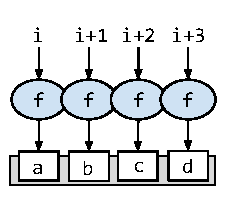
\includegraphics[width=2.6cm]{2-background/figs/Map} \\
  \texttt{\footnotesize{\textbf{Map}}} \\
\end{tabular}}
& \usebox{\MapHLL}
& \usebox{\MapPPL} \\ \hline
\vspace{-6pt} & & \\

\multirow{4}{*}{
\begin{tabular}{c}
  \vspace{-30pt} \\
  \texttt{\footnotesize{Indices}}\vspace{-6pt} \\
  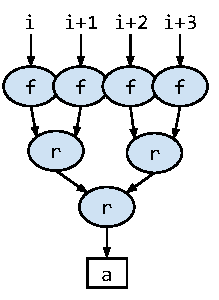
\includegraphics[width=2.6cm]{2-background/figs/Reduce} \\
  \texttt{\footnotesize{\textbf{MultiFold}}} \\
\end{tabular}\vspace{12pt}}
&
{\hspace{-6pt}\begin{tabular}{l}
\usebox{\MultiFoldHLLOne}  \\  \\
\end{tabular}}
& \usebox{\MultiFoldPPLOne} \\
\vspace{-6pt} & & \\
&
{\hspace{-6pt}\begin{tabular}{l}
\usebox{\MultiFoldHLLTwo} \\ \\ \\ \\
\end{tabular}}
& \usebox{\MultiFoldPPLTwo} \\
& & \\ \hline
\vspace{-6pt} & & \\

{\begin{tabular}{c}
  \texttt{\footnotesize{ Indices}}\vspace{-6pt} \\
  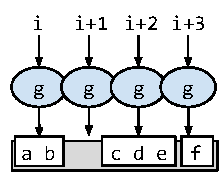
\includegraphics[width=2.6cm]{2-background/figs/FlatMap} \\
  \texttt{\footnotesize{\textbf{FlatMap}}} \\
\end{tabular}}
& \usebox{\FlatMapHLL}
& \usebox{\FlatMapPPL} \\ \hline
\vspace{-6pt} & & \\

{\begin{tabular}{c}
  \texttt{\footnotesize{  Indices}}\vspace{-6pt} \\
  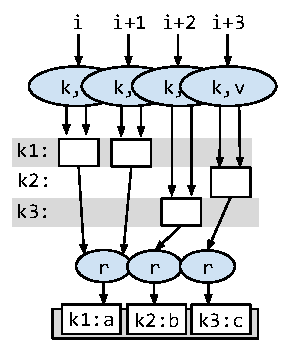
\includegraphics[width=3.2cm]{2-background/figs/HashReduce} \\
  \texttt{\footnotesize{\textbf{GroupByFold}}} \\
\end{tabular}}
& \usebox{\GroupByFoldHLL}
& \usebox{\GroupByFoldPPL} \\
\end{tabular}

\caption{\label{fig:ppl-examples}Usage examples for patterns in the PPL from various domain-specific languages.}
\end{figure*}


Figure~\ref{fig:ppl-examples} shows common examples of how users typically interact with
the patterns in PPL in various high level, domain specific languages
and how those examples are correspondingly represented in PPL. In some cases, the syntactic structure is
essentially the same except that the input domain is inferred from the shape of
the input collection. Using explicit indices in the intermediate language allows
us to model more user-facing patterns and more input access patterns with fewer internal primitives.

\emph{Map} generates a single element per index, aggregating the results into a fixed-size output collection.
Note that the value function can close over an arbitrary number of input collections, and therefore this pattern can represent classic parallel operations like \emph{map}, \emph{zip},
and \emph{zipWithIndex}.

\emph{MultiFold} is a generalization of a \emph{fold} which reduces generated values into a specified region of a (potentially) larger accumulator using an associative combine function.
The initial acummulator value $z$ is required to be an identity element of this function, and must have the same size and shape as the final output.
The main function $f$ generates an index specifying the location within the accumulator at which to reduce the generated value. We currently require the generated values to have the same arity as the full accumulator, but they may be of any size up to the size of the accumulator. Note that a traditional \emph{fold} is the special case of MultiFold where every generated value is the full size of the accumulator.
Function $f$ then converts each index into a function that consumes the specified
slice of the current accumulator and returns the new slice. If the pattern's
implementation maintains multiple partial accumulators in parallel, the combine
function $c$ reduces them into the final result.

\emph{FlatMap} generates an arbitrary number of values per index.
These values are all concatenated into a flattened output.
As the output size can only be determined dynamically, we restrict FlatMap to
one-dimensional domains so that dynamically growing the output is easily defined.
Note that this primitive also easily expresses a \emph{filter}.

\emph{GroupByFold} reduces generated values into one of many buckets where the bucket is selected by generating a key along with each value, i.e. it is a fused version of a \emph{groupBy} followed by a \emph{fold} over each bucket.
The operation is similar to \emph{MultiFold} except that the key-space cannot be determined in advance and so the output size is unknown.
Therefore we also restrict this operation to one-dimensional domains.




\begin{figure}
\centering
\begin{lstlisting}[language=Scala]
//data to be clustered, size n x d
val points: Array[Array[Float]] = ...

// current centroids, size k x d
val centroids: Array[Array[Float]] = ...

// Assign each point to the closest centroid by grouping
val groupedPoints = points.groupBy { pt1 =>
  // Assign current point to the closest centroid
  val minDistWithIndex = centroids.map { pt2 =>
    pt1.zip(pt2).map { case (a,b) => square(a - b) }.sum
  }.zipWithIndex.minBy(p => p._1)
  minDistWithIndex._2
}

// Average of points assigned to each centroid
val newCentroids = groupedPoints.map { case (k,v) =>
  v.reduce { (a,b) =>
    a.zip(b).map { case (x,y) => x + y }
  }.map { e => e / v.length }
}.toArray
\end{lstlisting}
\caption{K-Means clustering implemented using Scala collections. In Scala, \textunderscore\texttt{1} and \textunderscore\texttt{2} refer to the first and second value contained within a tuple.}
\label{fig:kmeans}
\end{figure}

\begin{figure}\centering
\begin{lstlisting}[language=Scala]
points: Array2D[Float](n,d)    // data to be clustered
centroids: Array2D[Float](k,d) // current centroids

// Sum and number of points assigned to each centroid
(sums,counts) = multiFold(n)((k,d),k)(zeros((k,d),k)){ i =>
  pt1 = points.slice(i, *)
  // Assign current point to the closest centroid
  minDistWithIndex = fold(k)((max, -1)){ j =>
    pt2 = centroids.slice(j, *)
    dist = fold(d)(0){ p =>
      acc => acc + square(pt1(p) - pt2(p))
    }{ (a,b) => a + b }
    acc => if (acc._1 < dist) acc else (dist, j)
  }{ (a,b) => if (a._1 < b._1) a else b }

  minDistIndex = minDistWithIndex._2
  sumFunc = ((minDistIndex, 0), acc => {
    pt = points.slice(i, *)
    map(d){ j => acc(j) + pt(j) }
  })
  countFunc = (minDistIndex, acc => acc + 1)

  (sumFunc, countFunc)
}{ (a,b) => {
  pt = map(k,d){ (i,j) => a._1(i,j) + b._1(i,j) }
  count = map(k){ i => a._2(i) + b._2(i) }
  (pt, count)
} }

// Average assigned points to compute new centroids
newCentroids = map(k,d){ (i,j) =>
  sums(i,j) / counts(i)
}
\end{lstlisting}
\caption{K-Means clustering represented using the parallel patterns in Figure~\ref{fig:ppl-syntax} after fusion and code motion.}
\label{fig:kmeans-fused}
\end{figure}

Now that we have defined the parallel pattern operations, we will use them to
implement example k-means clustering application.
For reference, first consider $k$-means implemented using the standard Scala
collections operations, as shown in Figure~\ref{fig:kmeans}.
$k$-means consumes a set of $n$ sample points of dimensionality $d$ and
attempts to cluster those points by finding the $k$ best cluster centroids for the samples.
This is achieved by iteratively refining the centroid values.
(We show only one iteration in Figure~\ref{fig:kmeans} for simplicity.)
First, every sample point is assigned to the closest current centroid by
computing the distance between every sample and every centroid.
Then new centroid values are computed by averaging all the samples assigned to each centroid.
This process repeats until the centroid values stop changing.
Previous work~\cite{rompf12optimizing,brown16clusters,chambers10flumejava} has shown how to stage a DSL application like $k$-means, lowering it into a parallel pattern IR similar to the one we define here, as well as how to perform multiple parallel pattern fusion automatically on the IR.
One of the most important of these optimizations is fusing patterns together, both vertically (to decrease the reuse distance between producer-consumer relationships) and horizontally (to eliminate redundant traversals over the same domain).
Figure~\ref{fig:kmeans-fused} shows the structure of $k$-means after it has been lowered into PPL and pattern fusion rules~\cite{rompf12optimizing} have been applied.
For simplicity, we have also converted the nested arrays in the Scala example to multidimensional arrays.
This translation requires the insertion of \emph{slice} operations in certain locations, which produce a view of a subset of the underlying data.
For the remainder of this work, we will assume the existence of a parallel pattern backend
for high level DSLs of interest and always start from the parallel pattern intermediate representation.

% \section{Field Programmable Gate Arrays}
%
% While this work will not attempt to give a comprehenesive description about how
% FPGAs are used or how they work, we will provide a short background

\chapter{Related Work}
\label{related}


\paragraph{Tiling}
Previous work on automated loop tiling has largely focused on tiling imperative programs
using polyhedral analysis~\cite{bondhugula08,pouchet10phd}.
There are many existing tools---such as Pluto~\cite{pluto08pldi},
PoCC~\cite{pouchet11popl}, CHiLL~\cite{chen2008chill},
and Polly~\cite{grosser2012polly}---that use polyhedral analysis
to automatically tile and parallelize programs.  These tools restrict memory
accesses within loops to affine functions of the loop iterators.
As a consequence, while they perform well on affine sections of programs,
they fail on commonly occurring data-dependent operations
like \emph{filters} and \emph{groupBys}~\cite{benabderrahmane10cc}. In order to handle these operations,
recent work has proposed using preprocessing steps which segment programs into affine
and non-affine sections prior to running polyhedral analysis tools~\cite{venkat}.

While the above work focused on the analysis of imperative programs, our work
analyzes functional parallel patterns, which offer a strictly higher-level representation
than simple imperative \emph{for} loops.
In this paper, we show that because of the additional semantic information
available in patterns like \emph{groupBy} and \emph{filter},
parallel patterns can be automatically tiled using
simple transformation rules, without the restriction that all memory accesses
are purely affine.
Little previous work has been done on automated tiling of functional
programs composed of arbitrarily nested parallel patterns.
Hielscher proposes a set of formal rules for tiling parallel operators \emph{map}, \emph{reduce}, and \emph{scan}
in the Parakeet JIT compiler, but these rules can be applied only for a small subset of nesting combinations \cite{parakeet}.
Spartan~\cite{spartan} is a runtime system with a set of high-level operators
(e.g., \emph{map} and \emph{reduce}) on multi-dimensional arrays, which
automatically tiles and distributes the arrays in a way that minimizes the
communication cost between nodes in cluster environments. In contrast to
our work, Spartan
operates on a tiled representation for distributed CPU computation and does attempt to optimize
performance on individual compute units.

%\begin{itemize}
%\item Tiling hyperplane method\cite{bondhugula08}
%\item Programming for Parallelism and Locality with Hierarchically Tiled Arrays \cite{bikshandi}
%\item Parameterized tiled loops for free\cite{renga07}
%\item Analytical bounds for optimal tile size selection\cite{shirako12}
%\item Tiling parallel patterns thesis
%\end{itemize}

%\textbf{Static modeling}
%\begin{itemize}
%\item Aladdin \cite{shao14}
%\end{itemize}

\paragraph{Hardware from high-level languages}
Generating hardware from high-level languages has been widely studied for
decades.  CHiMPS~\cite{chimps} generates hardware from ANSI C code by
mapping each C language construct in a data-flow graph to an HDL block.
Kiwi~\cite{kiwi} translates a set of C\# parallel constructs (e.g.,
\emph{event}, \emph{monitor}, and \emph{lock}) to corresponding hardware units.
Bluespec~\cite{bluespec} generates hardware from purely functional descriptions
based on Haskell.  Chisel~\cite{chisel} is an embedded language in Scala
for hardware generation.  AutoPilot~\cite{autopilot} is a commercial HLS
tool that generates hardware from C/C++/SystemC languages.  Despite their
success in raising the level of abstraction compared to hardware description
languages, programmers are still required to write programs at a low-level and
express how computations are pipelined and parallelized. Our work
abstracts away the implementation details from programmers by using high-level
parallel patterns, and applies compiler transformations to
automatically pipeline and parallelize operations and exploit on-chip memory
for locality.

Existing hardware synthesis tools are limited in their
ability to automatically infer and generate coarse-grained pipelines. A traditional
software pipelining approach is typically used on innermost loop bodies consisting
only of primitive operations. Optimizations like \emph{unroll-and-jam}, and \emph{unroll-and-squash}~\cite{unrollSquash}
also attempt to exploit pipelined parallelism, but target outer parallel loops
with inner sequential loops. To pipeline imperfectly nested loops, some
commercial high-level synthesis tools like Vivado~\cite{vivadohls} unroll all inner loops and then employ traditional
software pipelining. Not only does this approach generate needlessly large designs for large benchmarks,
it also suffers from long compilation times due to the complexity in scheduling a large number of unrolled instructions.
More recent works like ElasticFlow~\cite{elasticFlow} and CGPA~\cite{cgpa} generate coarse-grained
pipelines using FIFOs in between stages for communication. However, they handle only a restricted form of data access
patterns and a restricted number of nesting levels. Our metapipelining technique is more general than previous approaches because:
(i) metapipeline stages are decoupled using double buffers, therefore not restricting data access patterns, (ii) metapipelines
are easily composed and nested to any number of levels, and (iii) metapipelines can handle
dynamic rate mismatches as they use asynchronous handshaking for inter-stage synchronization, thereby obviating the need
to calculate static initiation interval as well as knowing loop trip counts ahead of time.


Recent work has explored using polyhedral analysis with HLS to optimize for data
locality on FPGAs~\cite{pouchet13fpga}.  Using polyhedral analysis, the compiler
is able to promote memory references to on-chip memory and parallelize
independent loop iterations with more hardware units.  However, the compiler is
not able to analyze loops that include non-affine accesses, limiting the
coverage of applications that can be generated for hardware. Our work can
handle parallel patterns with non-affine accesses by inferring required
hardware blocks (e.g., FIFOs and CAMs) for non-affine accesses, while
aggressively using on-chip memory for affine parts.

As high-level parallel patterns become increasingly popular to overcome the
shortcomings of C based languages, researchers have recently studied generating
hardware from functional parallel patterns.  Lime~\cite{auerbach10lime}
embeds high-level computational patterns (e.g., \emph{map}, \emph{reduce}, \emph{split}, and \emph{join}) in
Java and automatically targets CPUs, GPUs, and FPGAs without modifying the
code.  Our compiler manages a broader set of parallel patterns (e.g., \emph{groupBy})
and applies transformations even when patterns are nested,
which is common in a large number of real-world applications.  Recent work has
explored targeting nested parallel patterns to
FPGAs~\cite{george14fpl}. By exploiting the access patterns of nested patterns
to store sequential memory accesses to on-chip memory and parallelizing the
computation with strip-mining, the compiler can generate hardware that
efficiently utilizes memory bandwidth.  However, the compiler does not
automatically tile patterns for data locality or implement metapipelines
for nested parallel patterns, which we show are essential components for generating efficient hardware. Overall, our work is the first to show a complete method for
automatically tiling parallel patterns to improve locality for individual compute units and a process
for inferring hardware metapipelines from nested parallel patterns.

% We conclude with a qualitative comparison of Spatial to related work, drawing from the criteria in Section~\ref{background}.

%\gist{Here is what we believe are requirements of a good tool}
A good FPGA design tool should have the following features:
\begin{itemize}
  \item \emph{Representation}: The tool must internally represent hardware using a general and parameterizable
    representation. This representation must preserve information regarding data locality,
    memory access pattern and parallelism in the input at all levels of nesting.
    Such a representation must be target-agnostic and should be targetable from high-level
    language constructs.
  \item \emph{Estimation}: The tool must quickly analyze a design in the above representation
    and estimate metrics such as cycle counts and FPGA resource requirements for a target FPGA.
  \item \emph{DSE}: The tool must be able to leverage the estimators to prune the large design search space,
    walk the space of designs, and find the Pareto-optimal surface.
  \item \emph{Generation}: The tool must be able to automatically generate hardware which can then be
    synthesized and run on the target FPGA. Without this feature, hardware would typically
    be generated using separate toolchains for estimation and generation, which makes
    accurate estimation much harder.
\end{itemize}

Previous work on generating FPGA accelerators has focused on various aspects of the points
mentioned above. Here we provide an overview of this work.

High-level synthesis (HLS) tools such as LegUp~\cite{legup-tecs} and Vivado HLS~\cite{vivadohls} (previously AutoPilot)~\cite{cong11hls}
synthesize hardware from C. These tools provide estimates of the cycle count, area and power consumption
along with hardware generation. However, imperative design descriptions place greater burden on
the compiler to discover parallelism, pipeline structure and memory access patterns.
The absence of explicit parallelism often leads to conservative compiler analyses
producing sub-optimal designs. While some tools allow users to provide compiler
hints in the form of directives or pragmas in the source code, this approach
fails to capture key points in the design space.
\begin{figure}[ht]
  \begin{lstlisting}[mathescape=true, numbers=none, language=C]
L1: for (int i=0; i<R; i++) {
  #pragma HLS PIPELINE II=1
  L11: for (int j=0; j<C; j++) {
    sub[j] = y[i] ? x[i][j]-mu0[j] : x[i][j]-mu1[j];
  }
  L121: for (int j1=0; j1<C; j1++) {
    L122: for (int j2=0; j2<C; j2++) {
      sigma[j1][j2] += sub[j1]*sub[j2];
  }
}
  \end{lstlisting}
  \caption{GDA for high-level synthesis.}
  \label{fig:gda-hls}
\end{figure}
For example, consider Figure~\ref{fig:gda-hls} which represents the gaussian discriminant analysis (GDA)
kernel. All loops in this kernel are parallel loops. One set of valid design points would be to implement $L1$
as a coarse-grained pipeline with $L11$ and $L121$ as its stages. Commercial HLS tools support
 limited coarse-grained pipelining, but with serveral restrictions. For example,
the \emph{DATAFLOW} directive in Vivado HLS enables users to describe coarse-grained pipelines.
However, the directive does not support arbitrarily nested coarse-grained pipelines,
multiple producers and consumers between stages, or coarse-grain pipelining within a finite loop scope~\cite{vivadohls_ug}, as required in the outer loop in Figure~\ref{fig:gda-hls}.
%Such coarse-grained pipelining constructs are unfortunately not supported in most commercial
%HLS tools, leaving these design points unexplored.
%An attempt to pipeline $L1$ would create a large design with a deep pipeline where both $L11$ and $L121$
%are completely unrolled. % \todo{add some numbers}.
%This is a different design point than creating a coarse-grained pipeline.
In addition, compile times for HLS can be long for large designs due to the complications that
arise during scheduling. % \todo{add some numbers}.
Previous studies~\cite{Aladdin} point out other similar issues.
Such limitations restrict the capability of HLS tools to explore more complex design spaces.

Pouchet et al.~\cite{pouchet13fpga}
explore combining HLS with polyhedral analysis to optimize input designs for locality
and use estimates from HLS tools to drive design space exploration. While this captures a larger design
space than previous work by including tile sizes, this approach is limited to the capabilities
of the HLS tools and to benchmarks that have strictly affine data accesses. This paper improves
upon previous work by modeling tiling
parameters in addition to other design points like coarse-grained pipelining of imperfectly nested loops
which are not supported by HLS tools, as well as data-dependent accesses which are not supported by polyhedral analysis.
Chen et al.~\cite{cong_powerdse} describe a simultaneous resource allocation and binding algorithm
and perform design space exploration using a high-level power estimator. They characterize area
usage of primitives and fit linear models to derive estimation
functions. However, this study does not consider higher level design parameters or nested
parallelism as part of the design space. We perform characterization of primitive
operations as well as other coarse-grained templates, which enables us to estimate resource usage for
much more complex accelerators.
CMOST~\cite{cong_cmost} is a C-to-FPGA framework that uses task-level modeling
to exploit multi-level parallelism. While CMOST uses simple analytical models, this paper uses a mixture of
analytical and machine learning models that enables much more fine-grained and accurate estimation of FPGA resource utilization.

Aladdin\cite{Aladdin} is a pre-RTL estimation tool for ASIC accelerator design.
Aladdin uses a dynamic data dependence graph (DDDG) as input and estimates the latency, area, and power
for a variety of designs. However, using a DDDG limits the tool's ability to discover nested parallelism
and infer coarse-grained pipeline structures that require double buffering, especially with complex
memory accesses in patterns like \emph{filters} or \emph{groupBy}s. Also, Aladdin is focused on ASIC designs
while our work focuses on FPGA accelerators which have a different set of challenges, as outlined above.

Other related work~\cite{Deng,Bilavarn,MatchEst,Enzler,Bjureus} explore various ideas from analytical to empirical
models for estimating latency and area of designs in high-level languages. However, these approaches do not
consider complex applications with nested parallelism. Also, previous work either ignores memory or has a relatively
simple model for memory. This paper handles both on-chip and off-chip memory accesses
with varying, data-dependent memory access patterns.


\paragraph{HDLs}
Hardware description languages like Verilog and VHDL are designed for arbitrary circuit description. In order to achieve maximum generality, they require users to explicitly manage timing, control signals, and local memories. Loops are expressed by state machines in flattened RTL. 
One exception to this is Bluespec SystemVerilog \cite{bluespec}, which supports state machine inference from nested while loops.
Recent advancements in HDLs have largely been aimed at meta-programming improvements and increasing the size of hardware module libraries.
Languages like Chisel~\cite{chisel}, MyHDL~\cite{myhdl} and VeriScala~\cite{veriscala} make procedural generation of circuits simpler by embedding their HDL in a software language (e.g. Scala or Python). Similarly, Genesis2~\cite{genesis2} adds Perl scripting support to SystemVerilog to help drive procedural generation. While these improvements allow for more powerful meta-programming compared to Verilog \texttt{\small{generate}} statements, users still write programs at a timed circuit level.
%For application accelerators, such a low level of abstraction is often too tedious.


\paragraph{Lime}
Lime is a Java-based programming model and runtime from IBM which aims to provide a single unified language to program heterogeneous architectures. Lime natively supports custom bit precisions and includes collection operations, with parallelism in such operations inferred by the compiler. Coarse-grained pipeline and data parallelism are expressed through ``tasks''. Coarse-grained streaming computation graphs can be constructed using built-in constructs like \texttt{\small{connect}}, \texttt{\small{split}}, and \texttt{\small{join}}. The Lime runtime system handles buffering, partitioning, and scheduling of stream graphs. However, coarse-grained pipelines which deviate from the streaming model are not supported, and the programmer has to use a low-level messaging API to handle coarse-grained graphs with feedback loops. Additionally, the compiler does not perform automatic design tuning. Finally, the compiler's ability to instantiate banked and buffered memories is unclear as details on banking multi-dimensional data structures for arbitrary access patterns are not specified. 


\paragraph{HLS}
High-level synthesis tools such as LegUp~\cite{legup}, Vivado HLS~\cite{vivadohls}, Intel's FPGA SDK for OpenCL~\cite{opencl_sdk}, and SDAccel~\cite{sdaccel} allow users to write FPGA designs in C/C++ and OpenCL.
Using these tools, applications can be expressed at a high level, in terms of arrays and untimed, nested loops. 
However, while inner loop pipelining, unrolling, and memory banking and buffering are done by the compiler, they generally require explicit user pragmas.
While previous work has used polyhedral tools to automate banking decisions for affine accesses within a single loop nest~\cite{Wang_banking}, 
it does not address non-affine cases or cases where accesses to the same memory occur in multiple loop nests.
While pragmas like Vivado HLS's \emph{DATAFLOW} enable limited support for pipelining nested loops, pipelining at arbitrary loop nest levels is not yet supported~\cite{vivado_userguide}.
Tools like Aladdin~\cite{Aladdin} have also been created to help automate the process of tuning the pragmas in HLS programs, but designs in HLS still require manual hardware optimization~\cite{nane2016survey}.

%More importantly, users optimizing HLS describe their program in terms of arrays with pragmas. 
%While these are software constructs, optimizing hardware accelerators in HLS tools is a 
%Numerous issues, including memory aliasing, and low-level software implementation applications. 
%While most HLS tools primarily serve as IP core generators, but SDAccel \cite{sdaccel} is a systems-level solution. 
%Pragmas allow information to be added back to the compiler, but not in a sound way.  }

\paragraph{MaxJ}
MaxJ is a proprietary language created by Maxeler which allows users to express dataflow algorithms in Java libraries, emphasizing  
timing at the level of ``ticks`` of valid streaming elements rather than cycles. ~\cite{maxeler}. 
Users must fall back to flattened, HDL-like syntax for state machines when writing nested loops.
Memories are inferred based on relative stream offsets, which, while convenient for stream processing, 
hides hardware implementation details from the user which could otherwise help drive optimization.
Additionally, MaxJ has limited portability, as it currently can only be used to target supported Maxeler FPGA platforms. 

\paragraph{Image Processing DSLs}
Recently proposed image processing DSLs provide high-level specifications for targeting various
accelerator platforms, including GPUs and FPGAs.%~\cite{hegarty2014darkroom, membarth2016hipa, hegarty2016rigel, chugh2016dsl}.
The narrow domain allows these DSLs to offer more concise abstractions for specifying stencil operations. 
%Halide~\cite{pldi13halide}, for example, uses a declarative programming model which 
%entirely hides the loop structure of stencils from the programmer.
When targeting accelerators, these languages usually rely on source-to-source translation. 
$HIPA^{CC}$~\cite{membarth2016hipa}, for example, uses a
source-to-source compiler from a C-like front-end to generate CUDA, OpenCL, and Renderscript for
targeting GPUs. 
Recent work on Halide~\cite{pldi13halide} has demonstrated targeting heterogeneous systems, including the Xilinx Zynq's FPGA and ARM cores, by generating intermediate C++ and Vivado HLS~\cite{halidefpga}.
Rigel~\cite{hegarty2016rigel} and Darkroom~\cite{hegarty2014darkroom} generate Verilog, 
and PolyMage~\cite{chugh2016dsl} generates OpenMP and C++ for high-level synthesis. 
Rigel and Darkroom support generation of specialized memory structures on FPGAs, such as line buffers, in order to capture
reuse. $HIPA^{CC}$ can infer memory hierarchy on GPUs from a fix set of access patterns. 
These DSLs capture parallelism within a given stencil, typically across image channels 
and across the image processing pipeline.  

Compared to image processing DSLs, Spatial is more general and provides a 
lower level of abstraction. Spatial can express pipelining and unrolling for arbitrary loop hierarchies and explicitly exposes the memory hierarchy while automatically banking, buffering, and duplicating structures for arbitrary
access patterns. These features, along with Spatial's design tuning
capabilities, make Spatial a natural fit as an optimizing backend target for image processing DSLs.


% Compared to image processing DSLs, Spatial is
% more general but at a lower level of abstraction. Spatial uses a mix of imperative and functional specifications for stencil operations, 
% but is able to handle pipelining and unrolling for arbitrary loop hierarchies.
% Spatial requires explicit specification of the memory hierarchy, but is able to automatically bank, buffer, and duplicate for arbitrary access patterns.
% These features, along with Spatial's design space exploration capabilities, make Spatial a natural fit as an optimizing backend target for 
% image processing DSLs.

\chapter{High Level Compilation}

\section{Pattern Transformations}
\label{transformations}

One of the key challenges of generating efficient custom architectures from high level languages is in coping with arbitrarily large data structures. Since main memory accesses
are expensive and area is limited, our goal is to store a working set in the FPGA's local memory for as long as possible. Ideally, we also want
to hide memory transfer latencies by overlapping communication with computation using prefetching hardware blocks.
To this end, in this section we describe a method for automatically tiling parallel patterns to improve program locality and data reuse.
Like classic loop tiling, our pattern tiling method is composed of two transformations: strip mining and interchange.
We assume here that our input is a PPL representation of a program and that well known target-agnostic transformations like fusion, code motion, and struct unwrapping have already been run.

%Strip mining sequential, imperative loops is fairly straightforward.
%Due to the additional information inherent in parallel patterns, strip mining
\paragraph{Strip mining} %We first examine how parallel patterns can be strip mined.
%Simple imperative \emph{for} loops are strip mined using a single transformation rule: split the loop's domain to create a pair of nested \emph{for} loops.

%, and describes how tiles of the inner pattern should be combined into a
%representation equivalent to that created by the untiled pattern.
%The inner pattern is a transformed version of the original pattern which .
%In general, transformation rules on parallel patterns must preserve access pattern and parallelism information.
%In our intermediate representation, this necessitates that the strip mining rules  %outer loop created by strip mining a parallel pattern must itself be a parallel pattern.
%generate a set of perfectly nested parallel patterns.
The strip mining algorithm is defined here using two passes over the IR.
The first pass partitions each pattern's iteration domain \emph{d} into tiles of size \emph{b} by breaking the pattern into a pair of perfectly nested patterns.
The outer pattern operates over the strided index domain, expressed here as \emph{d/b}, while the inner pattern operates on a tile of size \emph{b}.
For the sake of brevity this notation ignores the case where \emph{b} does not perfectly divide \emph{d}.
This case is trivially solved with the addition of \emph{min} checks on the domain of the inner loop.
Table~\ref{table:stripmining} gives an overview of the rules used by transformer (denoted \emph{T}) to strip mine parallel patterns.
In addition to splitting up the domain, patterns are transformed by recursively strip mining all functions within that pattern.
Map is strip mined by reducing its domain and range and nesting it within a MultiFold. Note that the strided MultiFold writes
to each memory location only once. In this case we indicate the MultiFold's combination function as unused with an underscore.
As defined in Figure~\ref{fig:ppl-syntax}, the MultiFold, GroupByFold, and FlatMap patterns have the property that a perfectly nested form of a single instance of one of these
patterns is equivalent to a single ``flattened'' form of that same pattern. This property allows these patterns to be strip mined by
breaking them up into a set of perfectly nested patterns of the same type as the original pattern.

The second strip mining pass converts array slices and accesses with statically predictable access patterns into slices and accesses of larger, explicitly defined
array memory tiles. We define tiles which have a size statically known to fit on the FPGA using array copies.
Copies generated during strip mining can then be used to infer buffers during hardware generation.
%These buffers allow better usage of burst reads and writes from main memory and enable overlapping of compututation and communication using hardware prefetching.
Array tiles which have overlap, such as those generated from sliding windows in convolution, are marked with metadata in the IR as having some reuse factor.
Array copies with reuse have generation rules which minimize the number of redundant reads to main memory when possible.

\begin{table*}[t]
\small\centering
\begin{tabular}{@{}lll@{}}
\toprule
{\bf High Level Language}                            & {\bf PPL }       & {\bf Strip Mined PPL} \\ \midrule
{\begin{lstlisting}[numbers=none,language=Scala]
// Element-wise Map
val x: Array[Float] // length d
x.map{e => 2*e}
\end{lstlisting}}
&
{\begin{lstlisting}[numbers=none]
map(d){i => 2*x(i)}
\end{lstlisting}}
&
{\begin{lstlisting}[numbers=none]
multiFold(d/b)(d)(zeros(d)){ii =>
  xTile = x.copy(b + ii)
  (i, map(b)(b){i => 2*xTile(i) })
}(_)
\end{lstlisting}} \\ \midrule
{\begin{lstlisting}[numbers=none, language=Scala]
// Sums along matrix rows
val x: Array[Array[Float]] // m x n
x.map{ row =>
  row.fold(0){ (a,b) => a + b }
}
\end{lstlisting}}
&
{\begin{lstlisting}[numbers=none,language=PPL]
multiFold(m,n)(m)(zeros(m)){ (i,j) =>
  (i, acc => acc + x(i,j))
}{(a,b) =>
  map(n){(j) => a(j) + b(j)}
}
\end{lstlisting}}
&
{\begin{lstlisting}[numbers=none]
multiFold(m/b0,n/b1)(m)(zeros(m)){ (ii,jj) =>
  xTile = x.copy(b0 + ii, b1 + jj)
  tile = multiFold(b0,b1)(b0)(zeros(b0)){ (i,j) =>
    (i, acc => acc + xTile(i,j))
  }{(a,b) => map(b0){i => a(i) + b(i)} }
  (ii, acc => map(b0){j => acc(j) + tile(j)})
}{(a,b) =>
  multiFold(m/b0)(m)(zeros(m)){ii =>
    aTile = a.copy(b0 + ii)
    bTile = a.copy(b0 + ii)
    (ii, acc => map(b0){i => aTile(i) + bTile(i)})
  }{(a,b) => map(m){i => a(i) + b(i)}}
}
\end{lstlisting}} \\ \midrule
{\begin{lstlisting}[numbers=none]
// Simple Filter
val x: Array[Float] // length d
x.flatMap{ e =>
  if (e > 0) e else []
}
\end{lstlisting}}
&
{\begin{lstlisting}[numbers=none]
flatMap(d){i =>
  if (x(i) > 0) x(i) else []
}
\end{lstlisting}}
&
{\begin{lstlisting}[numbers=none]
flatMap(d/b)(1){ii =>
  eTile = x.copy(b + ii)
  flatMap(b){i =>
    if (eTile(i) > 0) eTile(i) else []
}}
\end{lstlisting}} \\ \midrule
{\begin{lstlisting}[numbers=none]
// Histogram Calculation
val x: Array[Float] // length d
x.groupByFold(0){ r =>
  (r/10, 1)
}{ (a,b) => a + b }
\end{lstlisting}}
&
{\begin{lstlisting}[numbers=none]
groupByFold(d)(0){i =>
  (x(i)/10, 1)
}{(a,b) => a + b }
\end{lstlisting}}
&
{\begin{lstlisting}[numbers=none]
groupByFold(d/b)(0){ii =>
  xTile = x.copy(b + ii)
  groupByFold(b)(0){i =>
    (xTile(i)/10, 1)
  }{(a,b) => a + b}
}{(a,b) => a + b}
\end{lstlisting}} \\ \bottomrule
\end{tabular}
\caption{Examples of the parallel pattern strip mining transformation on Map, MultiFold, FlatMap, and GroupByFold}
\label{table:stripmine-examples}
\end{table*}

\begin{table*}[t]
\centering\small
\begin{tabular}{@{}lll@{}}
\toprule
{\bf High Level Language}                            & {\bf Strip Mined PPL }       & {\bf Interchanged PPL} \\ \midrule
{\begin{lstlisting}[numbers=none]
// Matrix Multiplication
x: Array[Array[Float]] // m x p
y: Array[Array[Float]] // p x n
z = x.map{row =>
  y.map{col =>
    row.zipWith(col){(a,b) =>
      a * b
    }.sum
  }
}
\end{lstlisting}}
&
{\begin{lstlisting}[numbers=none]
multiFold(m/b0,n/b1)(m,n)(zeros(m,n)){(ii,jj) =>
(*@\color{vbgray}{\vrule}@*)  ((ii,jj), zTile =>
(*@\color{vbgray}{\vrule}@*)  (*@\color{vbgray}{\vrule}@*)  map(b0,b1){(i,j) =>
(*@\color{vbgray}{\vrule}@*)  (*@\color{vbgray}{\vrule}@*)  (*@\color{vbgray}{\vrule}@*)  tile = multiFold(p/b2)(1)(0){ kk =>
(*@\color{vbgray}{\vrule}@*)  (*@\color{vbgray}{\vrule}@*)  (*@\color{vbgray}{\vrule}@*)  (*@\color{vbgray}{\vrule}@*)  xTile = x.copy(b0 + ii, b2 + kk)
(*@\color{vbgray}{\vrule}@*)  (*@\color{vbgray}{\vrule}@*)  (*@\color{vbgray}{\vrule}@*)  (*@\color{vbgray}{\vrule}@*)  yTile = y.copy(b2 + kk, b1 + jj)
(*@\color{vbgray}{\vrule}@*)  (*@\color{vbgray}{\vrule}@*)  (*@\color{vbgray}{\vrule}@*)  (*@\color{vbgray}{\vrule}@*)  dprod = fold(b2)(0){ k =>
(*@\color{vbgray}{\vrule}@*)  (*@\color{vbgray}{\vrule}@*)  (*@\color{vbgray}{\vrule}@*)  (*@\color{vbgray}{\vrule}@*)  (*@\color{vbgray}{\vrule}@*)  acc => acc + xTile(i,k) * yTile(k,j)
(*@\color{vbgray}{\vrule}@*)  (*@\color{vbgray}{\vrule}@*)  (*@\color{vbgray}{\vrule}@*)  (*@\color{vbgray}{\vrule}@*)  }{(a,b) => a + b})
(*@\color{vbgray}{\vrule}@*)  (*@\color{vbgray}{\vrule}@*)  (*@\color{vbgray}{\vrule}@*)  (*@\color{vbgray}{\vrule}@*)  (0, elemTile => elemTile + dprod)
(*@\color{vbgray}{\vrule}@*)  (*@\color{vbgray}{\vrule}@*)  (*@\color{vbgray}{\vrule}@*)  }{(a,b) => a + b}
(*@\color{vbgray}{\vrule}@*)  (*@\color{vbgray}{\vrule}@*)  (*@\color{vbgray}{\vrule}@*)  zTile(i,j) + tile
(*@\color{vbgray}{\vrule}@*)  })
}(_)
\end{lstlisting}}
&
{\begin{lstlisting}[numbers=none]
multiFold(m/b0,n/b1)(m,n)(zeros(m,n)){(ii,jj) =>
(*@\color{vbgray}{\vrule}@*)  tile = multiFold(p/b2)(b0,b1)(...){kk =>
(*@\color{vbgray}{\vrule}@*)  (*@\color{vbgray}{\vrule}@*)  xTile = x.copy(b0 + ii, b2 + kk)
(*@\color{vbgray}{\vrule}@*)  (*@\color{vbgray}{\vrule}@*)  yTile = y.copy(b2 + kk, b1 + jj)
(*@\color{vbgray}{\vrule}@*)  (*@\color{vbgray}{\vrule}@*)  (0, elemTile =>
(*@\color{vbgray}{\vrule}@*)  (*@\color{vbgray}{\vrule}@*)  (*@\color{vbgray}{\vrule}@*)  map(b0,b1){(i,j) =>
(*@\color{vbgray}{\vrule}@*)  (*@\color{vbgray}{\vrule}@*)  (*@\color{vbgray}{\vrule}@*)  (*@\color{vbgray}{\vrule}@*)  dprod = fold(b2)(0){ k =>
(*@\color{vbgray}{\vrule}@*)  (*@\color{vbgray}{\vrule}@*)  (*@\color{vbgray}{\vrule}@*)  (*@\color{vbgray}{\vrule}@*)  (*@\color{vbgray}{\vrule}@*)  acc => acc + xTile(i,j) * yTile(j,k)
(*@\color{vbgray}{\vrule}@*)  (*@\color{vbgray}{\vrule}@*)  (*@\color{vbgray}{\vrule}@*)  (*@\color{vbgray}{\vrule}@*)  }{(a,b) => a + b}
(*@\color{vbgray}{\vrule}@*)  (*@\color{vbgray}{\vrule}@*)  (*@\color{vbgray}{\vrule}@*)  (*@\color{vbgray}{\vrule}@*)  elemTile(i,j) + dprod
(*@\color{vbgray}{\vrule}@*)  (*@\color{vbgray}{\vrule}@*)  })
(*@\color{vbgray}{\vrule}@*)  }{(a,b) =>
(*@\color{vbgray}{\vrule}@*)  (*@\color{vbgray}{\vrule}@*)  map(b0,b1){(i,j) => a(i,j) + b(i,j)
(*@\color{vbgray}{\vrule}@*)  }
(*@\color{vbgray}{\vrule}@*)  ((ii,jj), zTile =>
(*@\color{vbgray}{\vrule}@*)  (*@\color{vbgray}{\vrule}@*)  map(b0,b1){(i,j) => zTile(i,j) + tile(i,j)}
(*@\color{vbgray}{\vrule}@*)  })
}(_)
\end{lstlisting}} \\ \bottomrule
\end{tabular}
\caption{Example of the pattern interchange transformation applied to matrix multiplication.}
\label{table:interchange-examples}
\end{table*}


Table~\ref{table:stripmine-examples} demonstrates how our rules can be used to strip mine a set of simple data parallel operations.
We use the \emph{copy} infix function on arrays to designate array copies in these examples, using similar syntax as array \emph{slice}.
We assume in these examples that common subexpression elimination (CSE) and code motion transformation passes have been run after strip mining to eliminate duplicate copies and to
move array tiles out of the innermost patterns. In these examples, strip mining creates tiled copies of input collections that
we can later directly use to infer read buffers.

% \begin{table*}[t]\small\centering
% \begin{tabular}{@{}lll@{}}
% \toprule
% {\bf Nested Pattern }    & { }  & {\bf Interchanged Patterns} \\ \midrule
% {\begin{lstlisting}[mathescape=true,numbers=none]
% Map(d$_0$){i =>
%   MultiFold(d$_1$/b)(1)(z)(f)(c)
% }
% \end{lstlisting}
% } & \texttt{=>} &
% {\begin{lstlisting}[mathescape=true,numbers=none]
% MultiFold(d$_1$/b)(1)(Map(d$_0$)(z))(
%   (0, acc => Map(d$_0$){i => c(acc(i), f._2) })
% ){(a,b) => Map(d$_0$){i => c(a(i), b(i)) }}
% \end{lstlisting}
% } \\ \midrule
% {\begin{lstlisting}[mathescape=true,numbers=none]
% MultiFold(d$_0$)(d$_1$)(z)(
%   x = MultiFold(d$_1$/b)(d$_1$)(zeros(d$_1$))(f)(_)
%   (0, acc => MultiFold(d$_1$/b)(d$_1$)(zeros(d$_1$))(c(acc,x))(_))
% ){(a,b) =>
%   MultiFold(d$_1$/b)(d$_1$)(zeros(d$_1$))(c(a,b))(_)
% }
% \end{lstlisting}
% } & \texttt{=>} &
% {\begin{lstlisting}[mathescape=true,numbers=none]
% MultiFold(d$_1$/b)(d$_1$)(zeros(d$_1$))(
%   (0, acc => MultiFold(d$_0$)(1)(z)(f)(c) )
% )(_)
% \end{lstlisting}
% } \\ \bottomrule
% \end{tabular}
% \caption{Interchange transformation rules for pattern tiling.}
% \label{table:interchange}
% \end{table*}



\paragraph{Pattern interchange}
Given an intermediate representation with strip mined nested parallel patterns, we now need to interchange patterns to increase the reuse
of newly created data tiles. This can be achieved by moving strided patterns out of unstrided patterns. However, as with imperative loops,
it is not sound to arbitrarily change the order of nested parallel patterns.
We use two rules for pattern interchange adapted from a previously established \emph{Collect}-\emph{Reduce} reordering rule for computation on clusters~\cite{brown16clusters}.
These rules both match on the special case of MultiFold where every iteration updates the entire accumulator, which we refer to here as a \emph{fold}.
The first interchange rule defines how to move a scalar, strided \emph{fold} out of an unstrided Map, transforming the nested loop into a strided \emph{fold} of a Map.
Note that this also changes the combination function of the \emph{fold} into a Map.
The second rule is the inverse of the first, allowing us to reorder a strided MultiFold with no reduction function (i.e. the outer pattern of a tiled Map)
out of an unstrided \emph{fold}. This creates a strided MultiFold of a scalar \emph{fold}. We apply these two rules whenever possible to increase the reuse
of tiled inputs.
%The first rule defines how to reorder a Map out of

%ur pattern interchange rules are defined only on specific cases of perfectly nested patterns. These rules are given in Table~\ref{table:interchange}.
%Our rules define how to move
%a strided Fold out of an unstrided Map, creating a
%and a strided Map out of an unstrided Fold.


Imperfectly nested parallel patterns commonly occur either due to the way the original user program was structured or
as a result of aggressive vertical fusion run prior to tiling.
Interchange on imperfectly nested patterns requires splitting patterns into perfectly nested sections. However, splitting and reordering trades
temporal locality of intermediate values for increased reuse of data tiles. In hardware, this can involve creating more main memory
reads or larger on-chip buffers for intermediate results so that less reads need to be done for input and output data. This tradeoff between memory reads and
increased buffer usage requires more complex cost modeling.
We use a simple heuristic to determine whether to split fused loops: we split and interchange patterns only when
the intermediate result created after splitting and interchanging is statically known to fit on the FPGA. This handles the simple case
where the FPGA has unused on-chip buffers and allocating more on-chip memory guarantees a decrease in the number of main memory reads.
Future work will examine ways to statically model the tradeoff between main memory accesses and local buffers near 100\% on-chip memory utilization.


Table~\ref{table:interchange-examples} shows a simple example of the application of our pattern interchange rules on matrix multiplication.
We assume here that code motion has been run again after pattern interchange has completed.
In matrix multiplication, we interchange the perfectly nested strided MultiFold and the unstrided Map.
This ordering increases the reuse of the copied tile of matrix \emph{y} and changes the scalar reduction into a tile-wise reduction.
Note that the partial result calculation and the inner reduction can now be vertically fused.



\begin{figure*}\small\centering
%\begin{minipage}[b]{.4\textwidth}
\hspace{-0.105\textwidth}
\centering\begin{tabular}{cm{0.45\textwidth}m{0.01\textwidth}m{0.44\textwidth}}
{} &
{\begin{lstlisting}
(sums,counts) = multiFold(n/b0)((k,d),k)(...){ii =>
(*@\color{vbgray}{\vrule}@*)  pt1Tile = points.copy(b0 + ii, *)
(*@\color{vbgray}{\vrule}@*)  multiFold(b0)((k,d),k)(zeros(1,d),0){ i =>
(*@\color{vbgray}{\vrule}@*)  (*@\color{vbgray}{\vrule}@*)  pt1 = pt1Tile.slice(i, *)
(*@\color{vbgray}{\vrule}@*)  (*@\color{vbgray}{\vrule}@*)  minDistWithIndex = multiFold(k/b1)(1)((max, -1)){ jj =>
(*@\color{vbgray}{\vrule}@*)  (*@\color{vbgray}{\vrule}@*)  (*@\color{vbgray}{\vrule}@*)  pt2Tile = centroids.copy(b1 + jj, *)
(*@\color{vbgray}{\vrule}@*)  (*@\color{vbgray}{\vrule}@*)  (*@\color{vbgray}{\vrule}@*)  minIndTile = fold(b1)((max,-1)){ j =>
(*@\color{vbgray}{\vrule}@*)  (*@\color{vbgray}{\vrule}@*)  (*@\color{vbgray}{\vrule}@*)  (*@\color{vbgray}{\vrule}@*)  pt2 = pt2Tile.slice(j, *)
(*@\color{vbgray}{\vrule}@*)  (*@\color{vbgray}{\vrule}@*)  (*@\color{vbgray}{\vrule}@*)  (*@\color{vbgray}{\vrule}@*)  dist = distance(pt1, pt2)
(*@\color{vbgray}{\vrule}@*)  (*@\color{vbgray}{\vrule}@*)  (*@\color{vbgray}{\vrule}@*)  (*@\color{vbgray}{\vrule}@*)  acc => if (acc._1 < dist) acc else (dist, j+jj)
(*@\color{vbgray}{\vrule}@*)  (*@\color{vbgray}{\vrule}@*)  (*@\color{vbgray}{\vrule}@*)  }{ (a,b) => if (a._1 < b._1) a else b }
(*@\color{vbgray}{\vrule}@*)  (*@\color{vbgray}{\vrule}@*)  (*@\color{vbgray}{\vrule}@*)
(*@\color{vbgray}{\vrule}@*)  (*@\color{vbgray}{\vrule}@*)  (*@\color{vbgray}{\vrule}@*)  (0, acc =>
(*@\color{vbgray}{\vrule}@*)  (*@\color{vbgray}{\vrule}@*)  (*@\color{vbgray}{\vrule}@*)    if (acc._1 < minIndTile._1) acc else minIndTile)
(*@\color{vbgray}{\vrule}@*)  (*@\color{vbgray}{\vrule}@*)  }{(a,b) =>
(*@\color{vbgray}{\vrule}@*)  (*@\color{vbgray}{\vrule}@*)    if (a._1 < b._1) a else b
(*@\color{vbgray}{\vrule}@*)  (*@\color{vbgray}{\vrule}@*)  }
(*@\color{vbgray}{\vrule}@*)  (*@\color{vbgray}{\vrule}@*)
(*@\color{vbgray}{\vrule}@*)  (*@\color{vbgray}{\vrule}@*)
(*@\color{vbgray}{\vrule}@*)  (*@\color{vbgray}{\vrule}@*)  minDistIndex = minDistWithIndex._2
(*@\color{vbgray}{\vrule}@*)  (*@\color{vbgray}{\vrule}@*)  sumFunc = ... // Fig 4: lines 17-20
(*@\color{vbgray}{\vrule}@*)  (*@\color{vbgray}{\vrule}@*)  countFunc = ... // Fig 4: line 21
(*@\color{vbgray}{\vrule}@*)  (*@\color{vbgray}{\vrule}@*)  (sumFunc, countFunc)
(*@\color{vbgray}{\vrule}@*)  }{(a,b) => ... /* Tiled combination function */ }
(*@\color{vbgray}{\vrule}@*)  (0, acc => ... /* Tiled combination function */ )
}{(a,b) => ... /* Tiled combination function */ }

newCentroids = multiFold(k/b1,d)(k,d)(...){ (ii,jj) =>
(*@\color{vbgray}{\vrule}@*)  sumsBlk = sums.copy(b1 + ii, *)
(*@\color{vbgray}{\vrule}@*)  countsBlk = counts.copy(b1 + ii)
(*@\color{vbgray}{\vrule}@*)  (ii, acc => map(k,d){ (i,j) =>
(*@\color{vbgray}{\vrule}@*)    sumsBlk(i,j) / countsBlk(i)
(*@\color{vbgray}{\vrule}@*)  })
}
\end{lstlisting}} & \hfill &
%\end{minipage} \hfill
%\begin{minipage}[b]{.4\textwidth}
{\begin{lstlisting}
(sums,counts) = multiFold(n/b0)((k,d),k)(...){ ii =>
(*@\color{vbgray}{\vrule}@*)  pt1Tile = points.copy(b0 + ii, *)
(*@\color{vbgray}{\vrule}@*)  minDistWithInds = multiFold(k/b1)(b1)(map(b1)((max, -1))){ jj =>
(*@\color{vbgray}{\vrule}@*)  (*@\color{vbgray}{\vrule}@*)  pt2Tile = centroids.copy(b1 + jj, *)
(*@\color{vbgray}{\vrule}@*)  (*@\color{vbgray}{\vrule}@*)  minIndsTile = map(b0){ i =>
(*@\color{vbgray}{\vrule}@*)  (*@\color{vbgray}{\vrule}@*)  (*@\color{vbgray}{\vrule}@*)  pt1 = pt1Tile.slice(i, *)
(*@\color{vbgray}{\vrule}@*)  (*@\color{vbgray}{\vrule}@*)  (*@\color{vbgray}{\vrule}@*)  minIndTile = fold(b1)((max,-1)){ j =>
(*@\color{vbgray}{\vrule}@*)  (*@\color{vbgray}{\vrule}@*)  (*@\color{vbgray}{\vrule}@*)  (*@\color{vbgray}{\vrule}@*)  pt2 = pt2Tile.slice(j, *)
(*@\color{vbgray}{\vrule}@*)  (*@\color{vbgray}{\vrule}@*)  (*@\color{vbgray}{\vrule}@*)  (*@\color{vbgray}{\vrule}@*)  dist = distance(pt1, pt2)
(*@\color{vbgray}{\vrule}@*)  (*@\color{vbgray}{\vrule}@*)  (*@\color{vbgray}{\vrule}@*)  (*@\color{vbgray}{\vrule}@*)  acc => if (acc._1 < dist) acc else (dist, j+jj)
(*@\color{vbgray}{\vrule}@*)  (*@\color{vbgray}{\vrule}@*)  (*@\color{vbgray}{\vrule}@*)  }{ (a,b) => if (a._1 < b._1) a else b }
(*@\color{vbgray}{\vrule}@*)  (*@\color{vbgray}{\vrule}@*)  }
(*@\color{vbgray}{\vrule}@*)  (*@\color{vbgray}{\vrule}@*)  (0, acc => map(b0){ i =>
(*@\color{vbgray}{\vrule}@*)  (*@\color{vbgray}{\vrule}@*)    if (acc(i)._1 < minIndsTile(i)._1) acc else minIndsTile(i) })
(*@\color{vbgray}{\vrule}@*)  }{(a,b) =>
(*@\color{vbgray}{\vrule}@*)    map(b0){i => if (a(i)._1 < b(i)._1) a(i) else b(i) }
(*@\color{vbgray}{\vrule}@*)  }
(*@\color{vbgray}{\vrule}@*)  multiFold(b0)(k,d)(zeros(k,d)){ i =>
(*@\color{vbgray}{\vrule}@*)  (*@\color{vbgray}{\vrule}@*)  pt1 = pt1Tile.slice(i, *)
(*@\color{vbgray}{\vrule}@*)  (*@\color{vbgray}{\vrule}@*)  minDistIndex = minDistWithInds(i)._2
(*@\color{vbgray}{\vrule}@*)  (*@\color{vbgray}{\vrule}@*)  sumFunc = ... // Fig 4: lines 17-20
(*@\color{vbgray}{\vrule}@*)  (*@\color{vbgray}{\vrule}@*)  countFunc = ... // Fig 4: line 21
(*@\color{vbgray}{\vrule}@*)  (*@\color{vbgray}{\vrule}@*)  (sumFunc, countFunc)
(*@\color{vbgray}{\vrule}@*)  }{(a,b) => ... /* Tiled combination function */ }
(*@\color{vbgray}{\vrule}@*)  (0, acc => ... /* Tiled combination function */ )
}{(a,b) => ... /* Tiled combination function */ }

newCentroids = multiFold(k/b1,d)(k,d)(...){ (ii,jj) =>
(*@\color{vbgray}{\vrule}@*)  sumsBlk = sums.copy(b1 + ii, *)
(*@\color{vbgray}{\vrule}@*)  countsBlk = counts.copy(b1 + ii)
(*@\color{vbgray}{\vrule}@*)  (ii, acc => map(k,d){ (i,j) =>
(*@\color{vbgray}{\vrule}@*)    sumsBlk(i,j) / countsBlk(i)
(*@\color{vbgray}{\vrule}@*)  })
}
\end{lstlisting}}
\end{tabular}

\vspace{-0.2in}\begin{tabular}{cc}
{\parbox{0.45\textwidth}{\centering{(a) Strip mined $k$-means in PPL.}}} &
{\parbox{0.5\textwidth}{\centering{(b) Pattern Interchanged $k$-means in PPL.}}}
\end{tabular}

%\vspace{-0.045\textwidth}
\hspace{-0.180\textwidth}
\centering\begin{tabular}{cm{0.45\textwidth}m{0.01\textwidth}m{0.44\textwidth}}
{} &
{\begin{lstlisting}[numbers=none,language=Pseudo]
1     For each tile of b0 points:
2     (*@\color{vbgray}{\vrule}@*)  Copy the points tile into local memory
3 - 4 (*@\color{vbgray}{\vrule}@*)  (*@\textbf{\color{blue}{For each point \emph{pt1} in the points tile}}@*):
5     (*@\color{vbgray}{\vrule}@*)  (*@\color{vbgray}{\vrule}@*)  (*@\textbf{\color{red}{For each tile of b1 centroids}}@*):
6     (*@\color{vbgray}{\vrule}@*)  (*@\color{vbgray}{\vrule}@*)  (*@\color{vbgray}{\vrule}@*)  Copy the centroids tile into local memory
7 - 8 (*@\color{vbgray}{\vrule}@*)  (*@\color{vbgray}{\vrule}@*)  (*@\color{vbgray}{\vrule}@*)  For each centroid (*@\emph{pt2}@*) in the centroids tile:
9     (*@\color{vbgray}{\vrule}@*)  (*@\color{vbgray}{\vrule}@*)  (*@\color{vbgray}{\vrule}@*)  (*@\color{vbgray}{\vrule}@*)  Compute distance between (*@\emph{pt1}@*) and (*@\emph{pt2}@*)
10-11 (*@\color{vbgray}{\vrule}@*)  (*@\color{vbgray}{\vrule}@*)  (*@\color{vbgray}{\vrule}@*)  (*@\color{vbgray}{\vrule}@*)  Keep the closest (index,distance) pair
      (*@\color{vbgray}{\vrule}@*)  (*@\color{vbgray}{\vrule}@*)  (*@\color{vbgray}{\vrule}@*)  End
13-16 (*@\color{vbgray}{\vrule}@*)  (*@\color{vbgray}{\vrule}@*)  (*@\color{vbgray}{\vrule}@*)  Keep the closest pair across tiles
      (*@\color{vbgray}{\vrule}@*)  (*@\color{vbgray}{\vrule}@*)  End
20    (*@\color{vbgray}{\vrule}@*)  (*@\color{vbgray}{\vrule}@*)  Extract the index of the closest centroid
21    (*@\color{vbgray}{\vrule}@*)  (*@\color{vbgray}{\vrule}@*)  Add (*@\emph{pt1}@*) to row minDistIndex
22    (*@\color{vbgray}{\vrule}@*)  (*@\color{vbgray}{\vrule}@*)  Increment count at minDistIndex
24    (*@\color{vbgray}{\vrule}@*)  (*@\color{vbgray}{\vrule}@*)  Add point and count sums across tiles
      (*@\color{vbgray}{\vrule}@*)  End
25-26 (*@\color{vbgray}{\vrule}@*)  Add point and count sums across tiles
      End

28    For each tile of b1 point sums and counts:
29    (*@\color{vbgray}{\vrule}@*)  Copy the point sums tile into local memory
30    (*@\color{vbgray}{\vrule}@*)  Copy the point counts tile into local memory
31-32 (*@\color{vbgray}{\vrule}@*)  Compute each new centroid as sums(i) / count(i)
      End
\end{lstlisting}} & \hfill &
%\end{minipage} \hfill
%\begin{minipage}[b]{.4\textwidth}
{\begin{lstlisting}[numbers=none,language=Pseudo]
1     For each tile of b0 points:
2     (*@\color{vbgray}{\vrule}@*)  Copy the points tile into local memory
3     (*@\color{vbgray}{\vrule}@*)  (*@\color{red}{\textbf{For each tile of b1 centroids}}@*):
4     (*@\color{vbgray}{\vrule}@*)  (*@\color{vbgray}{\vrule}@*)  Copy the centroids tile into local memory
5 - 6 (*@\color{vbgray}{\vrule}@*)  (*@\color{vbgray}{\vrule}@*)  (*@\color{blue}{\textbf{For each point \emph{pt1} in the points tile}}@*):
7 - 8 (*@\color{vbgray}{\vrule}@*)  (*@\color{vbgray}{\vrule}@*)  (*@\color{vbgray}{\vrule}@*)  For each centroid (*@\emph{pt2}@*) in the centroids tile:
9     (*@\color{vbgray}{\vrule}@*)  (*@\color{vbgray}{\vrule}@*)  (*@\color{vbgray}{\vrule}@*)  (*@\color{vbgray}{\vrule}@*)  Compute distance between (*@\emph{pt1}@*) and (*@\emph{pt2}@*)
10-11 (*@\color{vbgray}{\vrule}@*)  (*@\color{vbgray}{\vrule}@*)  (*@\color{vbgray}{\vrule}@*)  (*@\color{vbgray}{\vrule}@*)  Keep the closest (index,distance) pair
      (*@\color{vbgray}{\vrule}@*)  (*@\color{vbgray}{\vrule}@*)  (*@\color{vbgray}{\vrule}@*)  End
      (*@\color{vbgray}{\vrule}@*)  (*@\color{vbgray}{\vrule}@*)  End
13-16 (*@\color{vbgray}{\vrule}@*)  (*@\color{vbgray}{\vrule}@*)  For each point: keep the closest pair across tiles
      (*@\color{vbgray}{\vrule}@*)  End
18-19 (*@\color{vbgray}{\vrule}@*)  (*@\color{blue}{\textbf{For each point \emph{pt1} in points tile}}@*):
20    (*@\color{vbgray}{\vrule}@*)  (*@\color{vbgray}{\vrule}@*)  Extract the index of the closest centroid
21    (*@\color{vbgray}{\vrule}@*)  (*@\color{vbgray}{\vrule}@*)  Add (*@\emph{pt1}@*) to row minDistIndex
22    (*@\color{vbgray}{\vrule}@*)  (*@\color{vbgray}{\vrule}@*)  Increment count at minDistIndex
24    (*@\color{vbgray}{\vrule}@*)  (*@\color{vbgray}{\vrule}@*)  Add point and count sums across tiles
      (*@\color{vbgray}{\vrule}@*)  End
25-26 (*@\color{vbgray}{\vrule}@*)  Add point and count sums across tiles
      End

28    For each tile of b1 point sums and counts:
29    (*@\color{vbgray}{\vrule}@*)  Copy the point sums tile into local memory
30    (*@\color{vbgray}{\vrule}@*)  Copy the point counts tile into local memory
31-32 (*@\color{vbgray}{\vrule}@*)  Compute each new centroid as sum / count
      End
\end{lstlisting}}
\end{tabular}


\vspace{-0.2in}\begin{tabular}{cc}
{\parbox{0.45\textwidth}{\centering{(c) Pseudocode description of strip mined $k$-means.}}} &
{\parbox{0.5\textwidth}{\centering{(d) Pseudocode description of pattern interchanged $k$-means.}}}
\end{tabular}

\vspace{0.1in}
\footnotesize{\begin{tabular}{|l|cc|cc|cc|}

\noalign{\hrule height 1.5pt}
\multicolumn{1}{|c|}{} & \multicolumn{2}{c|}{\bf Fused} & \multicolumn{2}{c|}{\bf Strip Mined}  & \multicolumn{2}{c|}{\bf Interchanged} \\
& Main Memory Reads & On-Chip Storage & Main Memory Reads & On-Chip Storage & Main Memory Reads & On-Chip Storage \\ \hline
\emph{points} & $n \times d$ & $d$ & $n \times d$ & $b_0 \times d$ & $n \times d$ & $b_0 \times d$ \\ \hline
\emph{centroids} & $n \times k \times d$ & $d$ & $n \times k \times d$ & $b_1 \times d$ & $(n/b_0) \times k \times d$ & $b_1 \times d$ \\ \hline
\emph{minDistWithIndex} & $0$ & $2$ & $0$ & $2$ & $0$ & $2 \times b_0$ \\
\noalign{\hrule height 1.5pt}
\end{tabular}}

\small
\vspace{0.1in}\centering{(e) Minimum number of words read from main memory and on-chip storage for data structures within $k$-means clustering after each IR transformation.}

%\end{minipage}
%\vspace{-0.1in}
%\centering\includegraphics[width=2.2in]{figs/tiledKmeans.pdf}
\caption{Full tiling example for $k$-means clustering, starting from the fused representation in Figure \ref{fig:kmeans-fused}, using tile sizes of \emph{b$_0$} and \emph{b$_1$} for the number of points $n$ and the number of clusters $k$. The number of features $d$ is not tiled in this example.}
\label{fig:kmeans-example}
\end{figure*}


\paragraph{Discussion}
The rules we outline here for automatic tiling of parallel patterns are target-agnostic. However, tile copies should only be made explicit
for devices with scratchpad memory. Architectures with hierarchical memory systems effectively maintain views of subsections of memory
automatically through caching, making explicit copies on these architectures a waste of both compute cycles and memory.

%We currently only support tiling of simple affine access and slicing patterns, where each index is either constant or of the form \emph{i + c},
%where \emph{i} is some parallel pattern index and \emph{c} is loop invariant. While this is only a subset of all affine accesses,
%these accesses are extremely common access pattern in the data analytics domain.
We currently require the user to explicitly specify tile sizes for all dimensions which require tiling. In future work, tile sizes for all pattern
dimensions will instead be determined by the compiler through automated tile size selection using modeling and design space exploration.

\paragraph{Example} We conclude this section with a complete example of tiling the $k$-means clustering algorithm, starting from the fused representation shown in Figure~\ref{fig:kmeans-fused}. We assume here that we wish
to tile the number of input points, \emph{n}, with tile size \emph{b$_0$} and the number of clusters, \emph{k}, with tile size \emph{b$_1$} but not the number of dimensions, \emph{d}. This is representative of machine learning
classification problems where the number of input points and number of labels is large, but the number of features for each point is relatively small.

Figure~\ref{fig:kmeans-example} gives a comparison of the $k$-means clustering algorithm after strip mining and after pattern interchange. During strip mining, we create
tiles for both the \emph{points} and \emph{centroids} arrays, which helps us to take advantage of main memory burst reads. However, in the strip mined version, we still fully
calculate the closest centroid for each point. This requires the entirety of \emph{centroids} to be read for each point. We increase the reuse of each tile of \emph{centroids} by first splitting
the calculation of the closest centroid label from the MultiFold (Figure~\ref{fig:kmeans-example}a. line~5). The iteration over the centroids tile is then perfectly nested within the iteration over the points. Interchanging these two iterations allows us to reuse the centroids tile across points, thus decreasing the total number of main memory reads for this array by a factor of \emph{b$_0$}. This decrease comes
at the expense of changing the intermediate (distance, label) pair for a single point to a set of intermediate pairs for an entire tile of \emph{points}. Since the created intermediate result
has size 2\emph{b$_0$}, we statically determine that this is an advantageous tradeoff and use the split and interchanged form of the algorithm.

\section{Hardware Generation}
\label{hardware}

In this section, we describe how the tiled intermediate representation is translated into an efficient FPGA design.
FPGAs are composed of various logic, register, and memory resources.
These resources are typically configured for a specific hardware design using a hardware description language (HDL) that is translated into an FPGA configuration file.
Our approach to FPGA hardware generation translates our parallel pattern IR into MaxJ, a Java-based hardware generation language (HGL), which is in turn used to generate an HDL.
This is simpler than generating HDL directly because MaxJ performs tasks such as automatic pipelining of innermost loops and other low-level hardware optimizations.

%In this section, we describe how the tiled intermediate representation is translated into efficient hardware.
%FPGAs are composed of various resources
%Programming FPGAs is typically done with a hardware description language, which is translated into a netlist

%Hardware generation uses a template-based approach to translate our parallel pattern IR into MaxJ HDL.

%Our approach targets architectures conforming to an abstract machine model where there is a large amount of off-chip slow memory connected to
%on-chip resources via one or more channels, limited amount of on-chip scratchpad memory, some
%compute resources, and the ability to synthesize multiple hierarchical Finite State Machines with Datapaths (FSMDs).

%%% Hardware templates here to make it at the top of the hardware gen page


\begin{table*}[t]
\footnotesize\centering
\begin{tabular}{ |m{1.5cm}|l|m{8cm}|m{3.8cm}| }

\noalign{\hrule height 1.5pt}
\multicolumn{1}{|l}{} &
\multicolumn{1}{c}{\bf Template} &
\multicolumn{1}{c}{\bf Description} &
\multicolumn{1}{c|}{\bf IR Construct} \\
\noalign{\hrule height 1.0pt}

\multirow{3}{1.5cm}[0pt]{\centering \bf Memories}
& Buffer & On-chip scratchpad memory & Statically sized array \\ \cline{2-4}
& Double buffer & Buffer coupling two stages in a metapipeline & Same as metapipeline controller \\ \cline{2-4}
& Cache & Tagged memory to exploit locality in random memory access patterns & Non-affine accesses \\
\noalign{\hrule height 1.0pt}

\multirow{4}{1.5cm}[0pt]{\centering \bf Pipelined Execution Units}
& Vector & SIMD parallelism & Map over scalars \\ \cline{2-4}
& Reduction tree & Parallel reduction of associative operations & MultiFold over scalars \\ \cline{2-4}
& Parallel FIFO & Used to buffer ordered outputs of dynamic size & FlatMap over scalars \\ \cline{2-4}
& CAM & Fully associative key-value store & GroupByFold over scalars \\
\noalign{\hrule height 1.0pt}
%\multicolumn{1}{|l|}{Priority Queue}          & \multicolumn{1}{p{7cm}|}{Pipelined priority insert into a list} & \multicolumn{1}{l|}{Sort} \\ \midrule

%\multicolumn{4}{|c|}{Controllers} \\ \midrule
\multirow{4}{1.5cm}[-10pt]{\centering \bf Controllers}
& Sequential & Controller which coordinates sequential execution & Sequential IR node \\ \cline{2-4}
& Parallel & Task parallel controller. Simultaneously starts all member modules when enabled, signals done when all members finish & Independent IR nodes \\ \cline{2-4}
& Metapipeline & Controller which coordinates execution of nested parallel patterns in a pipelined fashion & Outer parallel pattern with multiple inner patterns \\ \cline{2-4}
& Tile memory & Memory command generator to fetch tiles of data from off-chip memory & Transformer-inserted array copy \\
\noalign{\hrule height 1.5pt}

\end{tabular}
\caption{Hardware templates used in hardware code generation.}
\label{t-hwtemplates}
\end{table*}

Hardware generation follows a template-based approach. We analyze the structure of the parallel
patterns in the IR to determine the correct template to translate the pattern
to hardware. Table~\ref{t-hwtemplates} lists the templates and their corresponding IR constructs in three classes: memories, pipelined execution units,
and state machine controllers. \emph{Buffer}, \emph{Double buffer}, and \emph{Cache} are different on-chip memory
templates intended to capture both regular and data-dependent access patterns. In particular, the \emph{double buffer} template
is used to decouple execution stages and support dynamic rate mismatch between producer and consumer stages. Templates labeled as
\emph{Pipelined Execution Units} are used to support different kinds of innermost parallel patterns, as described in Table~\ref{t-hwtemplates}.
The \emph{Controller} templates implement a specific form of control flow using asynchronous handshaking signals. The \emph{Sequential},
\emph{Parallel}, and \emph{Metapipeline} controllers all orchestrate execution of a list of templates; \emph{Sequential} enforces
linear execution order, \emph{Parallel} enforces parallel execution with a barrier at the end, and \emph{MetaPipeline} enforces
pipelined execution. \emph{Tile Memory} controllers correspond to off-chip memory channels that load tiles of data into
one of the on-chip memory templates.
%We summarize the parallel pattern IR construct whose behavior each template captures in Table~\ref{t-hwtemplates}.
Each template can be composed with other templates.
For example, a \emph{Metapipeline controller} could be composed of multiple \emph{Parallel controller}s, each of which could
contain pipelined \emph{Vector} or \emph{Tree reduction} units.
%Next we discuss each of the templates in more detail.
We next describe the key features in the IR which we use to infer each of these template classes.



%\subsection{Memory Allocation}
\paragraph{Memory Allocation}
Generating efficient FPGA hardware requires effective usage of on-chip memories (buffers).
Prior to generating MaxJ, we run an analysis pass to allocate buffers for arrays based on data access patterns and size.
%Since the maximum size of data inputs can not usually be inferred statically, we support the use of programmer hints about tile sizes to aid this analysis.
%Information from these annotations is propagated through the IR during this analysis.
All arrays with statically known sizes, such as array \emph{copies} generated in the tiling transformation described in
Section~\ref{transformations}, are assigned to buffers. Dynamically sized arrays are kept in main memory and we generate
caches for any non-affine accesses to these arrays.
We also track each memory's readers and writers and use this information
to instantiate a template with the appropriate word width and number of ports.

% Special memories are used for buffers which have unique access patterns. Streaming or ``one-touch'' data is
% either streamed directly to and from off-chip memory or realized using FIFOs on-chip depending on their usage.
% The tiling transformations described in Section
% represent data tile copies with explicit nodes in the IR. This greatly simplifies memory allocation analysis.
% to first determine where data
% is stored and how it is accessed.
% The goal of this analysis is to assign buffers
% to either on-chip or off-chip memories and select a memory template based on the properties
% of the buffer.
%In general, we use the following heuristics to allocate memories:
%\begin{itemize}
%  \item Buffers which have statically unknown dimensions (typically inputs and outputs)
%    are allocated off-chip. However, we allow programmers to provide hints to the compiler using
%    annotations which can enable more aggressive compiler optimizations. For example, the programmer
%    can hint that a certain buffer is ``cacheable'' -- meaning that the size of the buffer is typically
%    small enough (a few Kilobytes) to completely fit on-chip. Our analysis makes use of this information
%    and performs more aggressive on-chip memory allocation.
%  \item Buffers corresponding to tiles are allocated on-chip.
%  \item
%  \item Intermediate buffers in a \emph{metapipeline} (described in the next section) are realized
%    using \emph{Double Buffers}.
%\end{itemize}

%While the memory allocation analysis performs an initial assignment of templates to buffers, certain special
%buffers need to be \emph{promoted} to use the double buffer template. This is determined during
%metapipeline analysis, described in the next section.


%\subsection{Pipeline Execution Units}
\paragraph{Pipeline Execution Units}
We generate parallelized and pipelined hardware when parallel patterns compute with scalar values,
as occurs for the innermost patterns.
We implemented templates for each
pipelined execution unit in Table~\ref{t-hwtemplates} using MaxJ language
constructs, and instantiate each template with the proper parameters (e.g., data type,
vector length) associated with the parallel pattern.  The MaxJ compiler
applies low-level hardware optimizations such as vectorization, code
scheduling, and fine-grained pipelining, and generates efficient hardware.  For
example, we instantiate a reduction tree for a MultiFold over an
array of scalar values, which is automatically pipelined by the MaxJ compiler.



%\subsection{Metapipelining}
\paragraph{Metapipelining}
To generate high performance hardware from parallel patterns, it is insufficient to exploit only a single level of parallelism.
However, exploiting nested parallelism requires mechanisms to orchestrate
the flow of data through multiple pipeline stages while also exploiting parallelism at each stage of execution,
creating a hierarchy of pipelines, or \emph{metapipeline}.
This is in contrast to traditional HLS tools which require inner patterns to have a static size and be completely unrolled in order to generate a flat pipeline containing both the inner and outer patterns.

% The main motivation behind metapipelining is to exploit parallelism at multiple levels of nesting. If
% a parallel pattern does not have other patterns in its body, then the pattern is implemented as a regular multi-stage
% dataflow pipeline. We leverage the pipelining constructs in the MaxJ programming language and the underlying
% MaxCompiler toolchain in order to implement these simpler pipelines.

%Pattern-specific rules to identify metapipeline stages are described in table \ref{table:metapipelineRules}.

%\todo{Introduce... Implementing a parallel pattern as a metapipeline involves multiple steps, as described below:}

\begin{figure*} \centering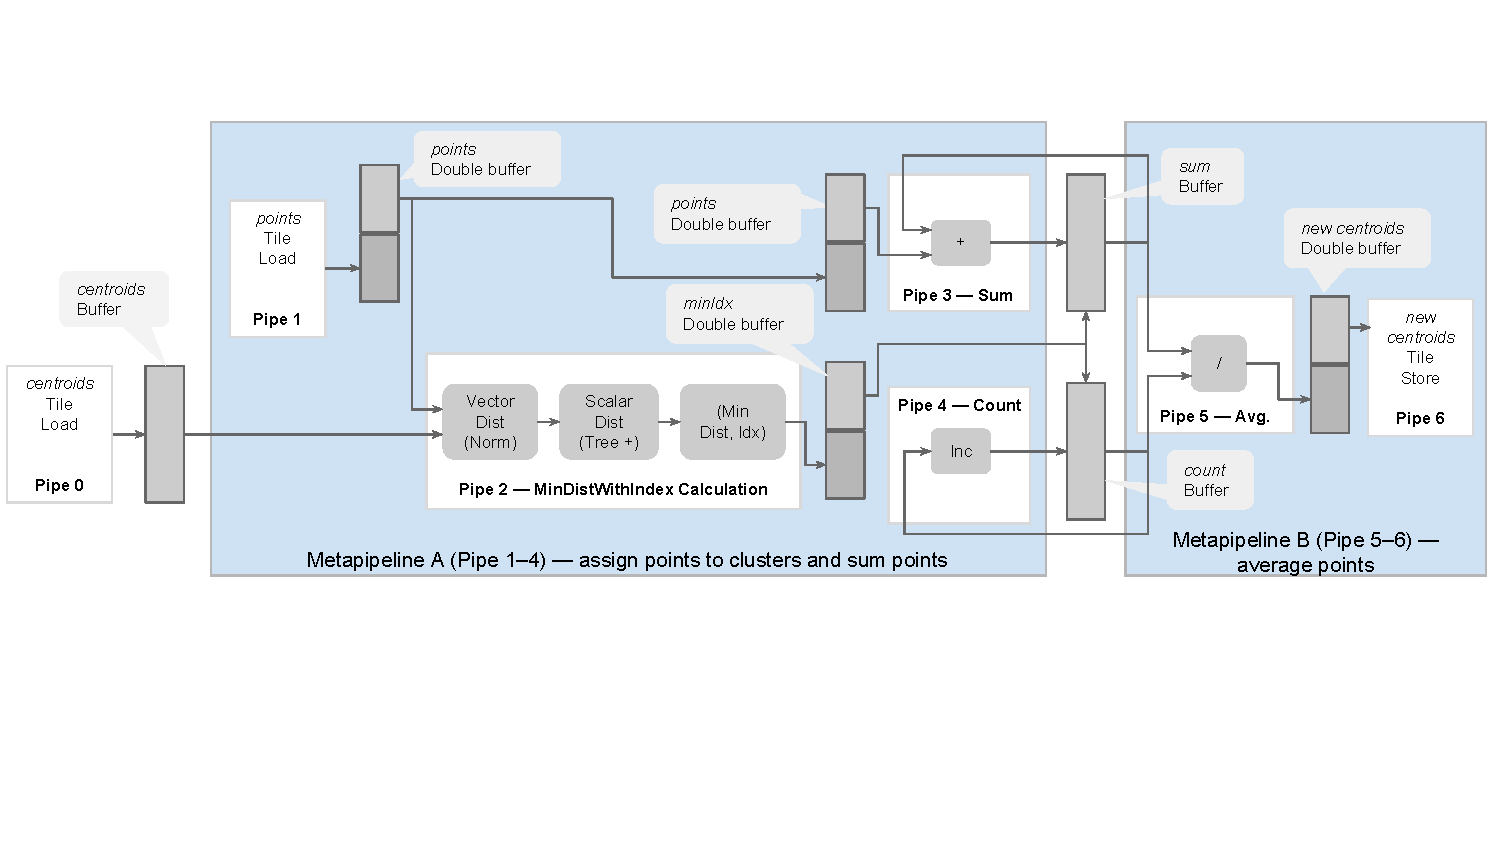
\includegraphics[clip=true,width=7in,trim=0in 0in
0in 0in]{figs/amazingmetapipelining.pdf}\caption{Hardware generated for the $k$-means application.}
\label{fig:metapipelining}
\end{figure*}

We create metapipeline schedules by first performing a topological sort on the IR of the body of the current parallel pattern.
The result is a list of stages, where each stage contains a list of patterns which can be run concurrently.
Exploiting the pattern's semantic information, we then
optimize the metapipeline schedule by removing unnecessary memory transfers and redundant computations.
For instance, if the output memory region of the pattern has been assigned to a buffer,
we do not generate unnecessary writes to main memory.

As another example, our functional representation of tiled parallel patterns can sometimes create redundant accumulation functions,
e.g., in cases where a MultiFold is tiled into a nested MultiFold. During scheduling we identify
this redundancy and emit a single copy of the accumulator, removing the unnecessary intermediate buffer.
Finally, in cases where the accumulator of a MultiFold cannot completely fit on-chip, we add a special
forwarding path between the stages containing the accumulator. This optimization avoids redundant writes to memory and
reuses the current tile.
Once we have a final schedule for the metapipeline, we promote every output buffer in each stage
to a double buffer to avoid write after read (WAR) hazards between metapipeline stages.


\paragraph{Example}
Figure~\ref{fig:metapipelining} shows a block diagram of the hardware generated for the $k$-means application.
For simplicity, this diagram shows the case where the \emph{centroids} array completely fits on-chip, meaning
we do not tile either the number of clusters \emph{k} or the number of features \emph{d}.
The generated hardware contains three sequential steps. The first step (Pipe~0) preloads the entire \emph{centroids} array into a buffer.
The second step (Metapipeline A) is a metapipeline which consists of three stages with double buffers to manage communication between the stages.
These three stages directly correspond to the three main sections of the MultiFold (Figure~\ref{fig:kmeans-fused}, line~5) used to sum and count the input points as grouped by their
closest centroid. The first stage (Pipe~1) loads a tile of the \emph{points} array onto the FPGA. Note that this stage is double buffered to
enable hardware prefetching. The second stage (Pipe~2) computes the index of the closest centroid using vector compute blocks and a scalar reduction
tree. The third stage (Pipe~3 and Pipe~4) increments the count for this minimum index and adds the current point to the corresponding location in the
buffer allocated for the \emph{new centroids}.
The third step (Metapipeline B) corresponds with the second outermost parallel pattern in the $k$-means application.
This step streams through the point sums and the centroid counts, dividing each sum by its corresponding count. The resulting new centroids
are then written back to main memory using a tile store unit for further use on the CPU.

Our automatically generated hardware design for the core computation of $k$-means is very similar to the manually optimized design described by Hussain et al.~\cite{hwkmeans}.
While the manual implementation assumes a fixed number of clusters and a small input dataset which can be preloaded onto the FPGA, we use tiling to automatically generate
buffers and tile load units to handle arbitrarily sized data. Like the manual implementation, we automatically parallelize across centroids
and vectorize the point distance calculations. As we see from the $k$-means example, our approach enables us to automatically generate high quality hardware implementations which are comparable to manual designs.

%Each of the pipes \todo{Complete kmeans example}

    %This is required so that when a pattern produces an output in one stage, a pattern in the
    %subsequent stage can safely and correctly read and operate on the produced data.
%\subsubsection{Controller Instantiation}
%    With the information from scheduling and optimization steps, we can instantiate a controller with
%    handshake signals to control the execution of each of its stages. At this time we also instantiate
%    intermediate double-buffered register files between each stage to propagate state information
%    such as iterator count, scalar values and other control signal information.

\section{Evaluation}
\label{evaluation}


\definecolor{bar1}{HTML}{5381BB}
\definecolor{bar2}{HTML}{BF4D4D}
\definecolor{bar3}{HTML}{9ABC5F}
\definecolor{bar4}{HTML}{8163A0}

We evaluate our approach to hardware generation described in Sections~\ref{transformations} and \ref{hardware} by comparing the performance and
area utilization of the FPGA implementations of a set of data analytic benchmarks.
We focus our investigation on the relative improvements that tiling and metapipelining provide over hardware designs that do not have these features.

\begin{figure*}[ht]
\centering
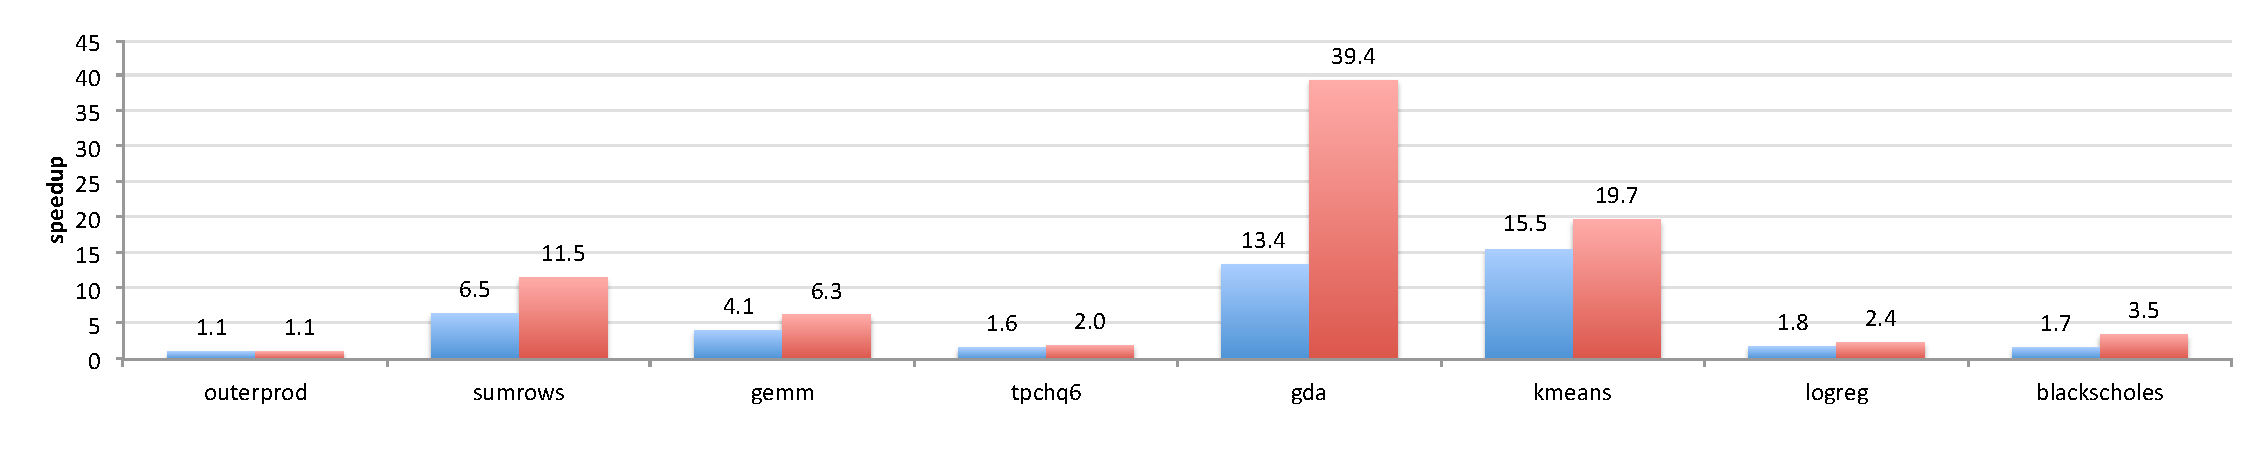
\includegraphics[width=\textwidth]{figs/newspeedupbars1.pdf}

\vspace{-10pt}

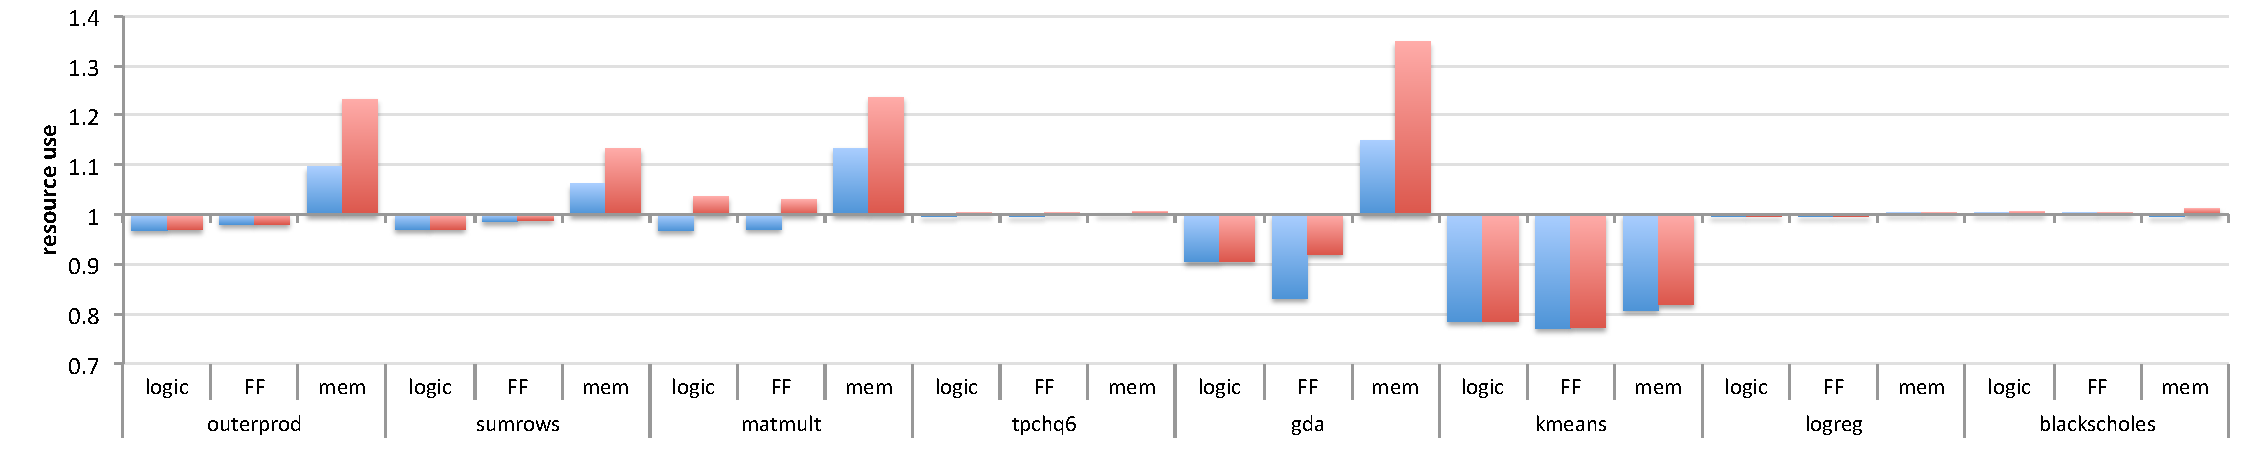
\includegraphics[width=\textwidth]{figs/newspeedupbars2.pdf}

{
\fontfamily{phv}\selectfont
\footnotesize
% \raisebox{-0.2em}{\tikz{\path[fill=bar3] (0,0) rectangle (2em,1em);}}
% base design
% \hspace{2em}
\raisebox{-0.2em}{\tikz{\path[fill=bar1] (0,0) rectangle (1em,1em);}}
+tiling
\hspace{2em}
\raisebox{-0.2em}{\tikz{\path[fill=bar2] (0,0) rectangle (1em,1em);}}
+tiling+metapipelining
}

\caption{Speedups and resource usages, relative to respective baseline designs, resulting from tiling and metapipelining.}
\label{fig:speedup-bars}
\end{figure*}

\begin{table}
\centering\footnotesize
\hspace{-0.022\textwidth}\begin{tabular}{lll}
\toprule

{\bf Benchmark} & {\bf Description} & {\bf Collections Ops}\\ \midrule
outerprod & Vector outer product & \emph{map}\\ \midrule
sumrows & Summation through matrix rows & \emph{map, reduce}\\ \midrule
gemm & Matrix multiplication & \emph{map, reduce}\\ \midrule
tpchq6 & TPC-H Query 6 & \emph{filter, reduce}\\ \midrule
%sobel & Sobel edge detection & Map \\ \midrule
logreg & Logistic regression & \emph{map, reduce}\\ \midrule
gda & Gaussian discriminant analysis & \emph{map, filter, reduce}\\ \midrule
blackscholes & Black-Scholes option pricing & \emph{map}\\ \midrule
kmeans & $k$-means clustering & \emph{map, groupBy, reduce}\\ \bottomrule
%knn & k Nearest Neighbors & MultiFold, Map, GroupByFold \\ \bottomrule
\end{tabular}

\caption{Evaluation benchmarks with major collections operations used by
Scala implementation.}
\label{table:benchmarks}
\end{table}

\subsection{Methodology}
The benchmarks used in our evaluation are summarized in Table~\ref{table:benchmarks}.
We choose to study vector outer product, matrix row summation, and matrix multiplication as these exemplify many commonly occurring access patterns in the machine learning domain.
TPC-H Query 6 is a data querying application which reads a table of purchase records, filtering all
records which match a given predicate. It then computes the sum of a product of two columns in the filtered records.
Logistic regression is a binary discriminative classification algorithm that uses the sigmoid function in the calculation of predictions.
Gaussian discriminant analysis (GDA) is a classification algorithm which models the distribution of each class as a multivariate Gaussian.
Black-Scholes is a financial analytics application for option pricing.
$k$-means clustering groups a set of input points by iteratively calculating the $k$ best cluster centroids.
In our implementations, all of these benchmarks operate on single precision, floating point data.

We implement our transformation and hardware generation steps in an existing compiler framework called Delite~\cite{delite-tecs14}.
We write each of our benchmark applications in OptiML~\cite{optiml}, a high level, domain specific language embedded in Scala for machine learning.
We then compile each of these applications with the modified Delite compiler.
During compilation, applications are staged, translating them into PPL representations.
%Delite represents programs as a directed graph of compute nodes and communication edges.
%Parallel patterns are explicitly represented as compute nodes in Delite, enabling coarse grain optimizations and analyses like the ones we describe in section \ref{transformations}.
%Keeping with our generative programming model,
The compiler then performs the tiling transformations and hardware optimizations described in Sections \ref{transformations} and \ref{hardware} before generating MaxJ hardware designs.
We then use the Maxeler MaxCompiler toolchain to generate an FPGA configuration bitstream from our generated MaxJ. We use the Maxeler runtime layer to manage communication with the FPGA from the host CPU.
%These VHDL descriptions are compiled to a final FPGA configuration bitstream by Altera synthesis tools.
%Delite also links in C libraries for handling file reading, transferring data between CPU DRAM and FPGA DRAM, and configuring the FPGA with the generated bitstream.
We measure the running times of these designs starting after input data has been copied to the FPGA's DRAM and ending when the hardware design reports completion.
Final running times were calculated as an arithmetic mean of five individual run times to account for small runtime variations in main memory accesses and Maxeler's device driver stack.

We run each generated design on an Altera Stratix V FPGA on a Max4 Maia board.
The Maia board contains 48~GB of DDR3 DRAM with a maximum bandwidth of 76.8~GB/s.
The area numbers given in this section are obtained from synthesis reports provided by Altera's logic synthesis toolchain.
Area utilization is reported under three categories: Logic utilization (denoted ``logic''), flip flop usage (``FF''), and on-chip memory usage (``mem'').

%created by Maxeler Technologies. The MaxJ language allows users to specify a dataflow description of their hardware design.
%\todo{brief sentence or two about MaxJ as an abstraction for hardware between HDL and our parallel patterns}



\subsection{Experiments}
The baseline for each benchmark is an optimized hardware design implemented using MaxJ.
The baseline designs were manually tuned after automatic generation and are
representative of optimizations done by state-of-the-art high-level synthesis tools.
In particular, each baseline design exploits data and pipelined parallelism within patterns where possible.
Pipelined parallelism is exploited for patterns that operate on scalars. Our baseline design
exploits locality at the level of a single DRAM burst, which on the MAX4 MAIA board is 384 bytes.
To isolate the effects of the amount of parallelism in our comparison, we keep
the innermost pattern parallelism factor constant between the baseline design and our optimized versions for each benchmark.


We evaluate our approach against the baseline by generating two hardware configurations per benchmark:
a configuration with tiling but no metapipelining, and a configuration with both tiling and metapipelining optimizations enabled.
%\todo{Reasoning as to why we don't show metapipelining alone?}

\paragraph{Impact of tiling alone}
Figure \ref{fig:speedup-bars} shows the obtained speedups as well as relative on-chip resource utilizations for each of benchmarks.
As can be seen, most benchmarks in our suite show significant speedup when tiling
transformations are enabled. Benchmarks like \emph{sumrows} and \emph{gemm}
benefit from inherent locality in their memory accesses. For \emph{gemm}, our automatically generated code
achieves a speedup of $4\times$ speedup over the baseline for a marginal increase of about $10\%$ on-chip memory usage.

%Note, the baseline for \emph{gemm} also exploits locality
%by using a tiling where the number of columns in each tile is equal to one DRAM burst. This means that our baseline
%uses tile sizes $1 \times 96 \times 96$.

Benchmarks \emph{outerprod} and \emph{tpchq6} do not
show a significant difference with our tiling transformations over the baseline.
This is because both \emph{outerprod} and
\emph{tpchq6} are both memory-bound benchmarks. \emph{Tpchq6} streams through the input once without reuse, and streaming
data input is already exploited in our baseline design. \emph{Blackscholes} has a similar data access pattern as \emph{tpchq6},
due to which it achieves a speedup similar to that of \emph{tpchq6}. Hence tiling does not provide any additional benefit.
Most of the locality in \emph{logreg} is already captured at burst-level granularity by our baseline. As a result, \emph{logreg}
achieves a modest speedup of $1.8x$ over the baseline due to tiling.
The core compute pipeline in \emph{outerprod} is memory-bound at the stage writing results to DRAM, which cannot be addressed
using tiling. Despite the futility of tiling in terms of performance, tiling \emph{outerprod}
has a noticeable increase in memory utilization as the intermediate result varies as the square of the tile size.

In \emph{kmeans} and \emph{gda}, some
of the input data structures are small enough that they can be held in on-chip memory. This completely
eliminates accesses to off-chip memory, leading to dramatic speedups of $13.4\times$ and $15.5\times$ respectively
with our tiling transformations. \emph{gda} uses more on-chip memory to store intermediate data. On the other hand, the tiled
version \emph{kmeans} utilizes less on-chip memory resources. This is because the baseline for \emph{kmeans} instantiates multiple
load and store units, each of which creates several control structures in order to read and write data from DRAM. Each of these control
structures includes address and data streams, which require several on-chip buffers. By tiling, we require a smaller number of load and
store units.

\paragraph{Impact of metapipelining}
The second speedup bar in Figure~\ref{fig:speedup-bars} shows the benefits of metapipelining. Metapipelines increase throughput
at the expense of additional on-chip memory used for double buffers.
Metapipelining overlaps design compute with data transfer and helps to hide the cost of the slower stage. Benchmarks like
\emph{gemm} and \emph{sumrows} naturally benefit from metapipelining because the memory transfer time is completely overlapped
with the compute, resulting in speedups of $6.3\times$ and $11.5\times$ respectively. Metapipelining also exploits overlap in
streaming benchmarks like \emph{tpchq6} and \emph{blackscholes}, where the input data is fetched and stored simultaneously with the core computation.

The speedup due to metapipelining is largely determined by balancing between stages. Stages with roughly equal number of cycles benefit
the most, as this achieves the most overlap. Unbalanced stages are limited by the slowest stage, thus limiting performance.
We observe this behavior in \emph{outerprod},
where the metapipeline is bottlenecked by the stage writing results back to DRAM. The metapipeline in \emph{logreg} is bottlenecked
at the stage performing dot products of all the points in the input tile with the \emph{theta} vector. As we only parallelize the
innermost parallel pattern in this work, only a single dot product is produced at a time, even though the dot product itself
is executed in parallel across the point dimensions. On the other hand, applications
like \emph{gda}, \emph{kmeans} and \emph{sumrows} greatly benefit from metapipelining. In particular, \emph{gda} naturally
maps to nested metapipelines that are well-balanced. The stage loading the input tile overlaps execution with the stage
computing the output tile and the stage storing the output tile. The stage computing the output tile is also
a metapipeline where the stages perform vector subtraction, vector outer product and accumulation. We parallelize the vector
outer product stage as it is the most compute-heavy part of the algorithm; parallelizing the vector outer product enables
the metapipeline to achieve greater throughput. This yields an overall speedup of $39.4\times$
over the baseline.

\chapter{Spatial}
\label{spatial}

\section{The Spatial Language}
\label{language}

Spatial is a domain specific language for the design of accelerators implemented on reconfigurable spatial architectures, including FPGAs and CGRAs. 
The aim of the language is to simplify the accelerator design process, 
allowing domain experts to quickly develop, test, optimize, and deploy hardware accelerators, either by 
directly implementing high-level hardware designs or by targeting Spatial from another, higher level language.

%When used to target FPGAs, the output of Spatial is a target-specific, synthesizable Chisel project, meaning users can go directly from a Spatial program to a design running on their target device.
%Spatial is currently implemented as an embedded language in Scala. 
%Spatial employs a mix of imperative and functional paradigms to improve the amount of information available to the compiler.
In this section, we describe the abstractions Spatial includes to balance productivity and performance-oriented detail.
While space does not permit a full specification of the language, Table~\ref{t:syntaxTable} provides an overview of the core subset of Spatial's syntax. 
%including control structures, optional user scheduling directives, memory templates for various levels of the memory hierarchy, and design space parameters.


%A higher level language targeted towards hardware accelerator design must strike the right balance
%between high-level abstractions for improving programmer productivity and target-specific constructs for controlling hardware performance. 

%In this section, we discuss several of the key challenges in defining hardware accelerator designs and describe abstractions the Spatial language includes to place the burden of this complexity on the compiler rather than the application programmer.


\begin{table*}
\centering
\caption{A subset of Spatial's syntax.
%An overview of Spatial's syntax for host interfaces, control structures, scheduling directives, memory templates, streaming interfaces, and design space parameters. 
Square brackets (e.g. \texttt{[T]}) represent a template's type parameter. Parameters followed by a `\texttt{+}' denote arguments which can be given one or more times, while a `\texttt{*}' denotes that an argument is optional. 
\texttt{DRAMs}, \texttt{Foreach}, \texttt{Reduce}, and \texttt{MemReduce} can all have arbitrary dimensions. 
%\texttt{DRAMs} can be allocated with an arbitrary number of dimensions. \texttt{Foreach}, \texttt{Reduce}, and \texttt{MemReduce} support multi-dimensional iteration domains. 
}
\label{t:syntaxTable}


\newsavebox{\counter}
\begin{lrbox}{\counter}
\begin{lstlisting}[language=SpatialTable]
min* until max by stride* par factor*
\end{lstlisting}
\end{lrbox}

\newsavebox{\fsmSignature}
\begin{lrbox}{\fsmSignature}
\begin{lstlisting}[language=SpatialTable]
FSM(init){continue}{action}{next}
\end{lstlisting}
\end{lrbox}

\newsavebox{\foreachSignature}
\begin{lrbox}{\foreachSignature}
\begin{lstlisting}[language=SpatialTable]
Foreach(counter+){body}
\end{lstlisting}
\end{lrbox}

\newsavebox{\reduceSignature}
\begin{lrbox}{\reduceSignature}
\begin{lstlisting}[language=SpatialTable]
Reduce(accum)(counter+){func}{reduce}
\end{lstlisting}
\end{lrbox}

\newsavebox{\memreduceSignature}
\begin{lrbox}{\memreduceSignature}
\begin{lstlisting}[language=SpatialTable]
MemReduce(accum)(counter+){func}{reduce}
\end{lstlisting}
\end{lrbox}

\newsavebox{\streamStar}
\begin{lrbox}{\streamStar}
\begin{lstlisting}[language=SpatialTable]
Stream(*){body}
\end{lstlisting}
\end{lrbox}

\newsavebox{\parallelSignature}
\begin{lrbox}{\parallelSignature}
\begin{lstlisting}[language=SpatialTable]
Parallel{body}
\end{lstlisting}
\end{lrbox}

\newsavebox{\pipeSignature}
\begin{lrbox}{\pipeSignature}
\begin{lstlisting}[language=SpatialTable]
DummyPipe{body}
\end{lstlisting}
\end{lrbox}

\newsavebox{\ifSignature}
\begin{lrbox}{\ifSignature}
\begin{lstlisting}[language=SpatialTable]
if (cond){body} 
[else if (cond){body} ] 
[else {body} ]
\end{lstlisting}
\end{lrbox}

\newsavebox{\sequentialTag}
\begin{lrbox}{\sequentialTag}
\begin{lstlisting}[language=SpatialTable]
Sequential.(Foreach|Reduce|MemReduce)
\end{lstlisting}
\end{lrbox}

\newsavebox{\pipeTag}
\begin{lrbox}{\pipeTag}
\begin{lstlisting}[language=SpatialTable]
Pipe(ii*).(Foreach|Reduce|MemReduce)
\end{lstlisting}
\end{lrbox}

\newsavebox{\streamTag}
\begin{lrbox}{\streamTag}
\begin{lstlisting}[language=SpatialTable]
Stream.(Foreach|Reduce|MemReduce)
\end{lstlisting}
\end{lrbox}

\newsavebox{\parallelTag}
\begin{lrbox}{\parallelTag}
\begin{lstlisting}[language=SpatialTable]
Parallel.(Foreach|Reduce|MemReduce)
\end{lstlisting}
\end{lrbox}

\newsavebox{\fifoSyntax}
\begin{lrbox}{\fifoSyntax}
\begin{lstlisting}[language=SpatialTable]
FIFO[T](depth)
\end{lstlisting}
\end{lrbox}

\newsavebox{\filoSyntax}
\begin{lrbox}{\filoSyntax}
\begin{lstlisting}[language=SpatialTable]
LIFO[T](depth)
\end{lstlisting}
\end{lrbox}

\newsavebox{\lineBufferSyntax}
\begin{lrbox}{\lineBufferSyntax}
\begin{lstlisting}[language=SpatialTable]
LineBuffer[T](r, c)
\end{lstlisting}
\end{lrbox}

\newsavebox{\lutSyntax}
\begin{lrbox}{\lutSyntax}
\begin{lstlisting}[language=SpatialTable]
LUT[T](dims+)(elements+)
\end{lstlisting}
\end{lrbox}

\newsavebox{\regSyntax}
\begin{lrbox}{\regSyntax}
\begin{lstlisting}[language=SpatialTable]
Reg[T](reset*)
\end{lstlisting}
\end{lrbox}

\newsavebox{\regfileSyntax}
\begin{lrbox}{\regfileSyntax}
\begin{lstlisting}[language=SpatialTable]
RegFile[T](dims+)
\end{lstlisting}
\end{lrbox}

\newsavebox{\sramSyntax}
\begin{lrbox}{\sramSyntax}
\begin{lstlisting}[language=SpatialTable]
SRAM[T](dims+)
\end{lstlisting}
\end{lrbox}

\newsavebox{\argInSyntax}
\begin{lrbox}{\argInSyntax}
\begin{lstlisting}[language=SpatialTable]
ArgIn[T]
\end{lstlisting}
\end{lrbox}

\newsavebox{\argOutSyntax}
\begin{lrbox}{\argOutSyntax}
\begin{lstlisting}[language=SpatialTable]
ArgOut[T]
\end{lstlisting}
\end{lrbox}

\newsavebox{\hostIOSyntax}
\begin{lrbox}{\hostIOSyntax}
\begin{lstlisting}[language=SpatialTable]
HostIO[T]
\end{lstlisting}
\end{lrbox}

\newsavebox{\dramSyntax}
\begin{lrbox}{\dramSyntax}
\begin{lstlisting}[language=SpatialTable]
DRAM[T](dims+)
\end{lstlisting}
\end{lrbox}

\newsavebox{\streamInSyntax}
\begin{lrbox}{\streamInSyntax}
\begin{lstlisting}[language=SpatialTable]
StreamIn[T](bus)
\end{lstlisting}
\end{lrbox}

\newsavebox{\streamOutSyntax}
\begin{lrbox}{\streamOutSyntax}
\begin{lstlisting}[language=SpatialTable]
StreamOut[T](bus)
\end{lstlisting}
\end{lrbox}

\newsavebox{\parameterSyntax}
\begin{lrbox}{\parameterSyntax}
\begin{lstlisting}[language=SpatialTable]
default (min,max)
default (min,stride,max)
\end{lstlisting}
\end{lrbox}

\newsavebox{\accelSyntax}
\begin{lrbox}{\accelSyntax}
\begin{lstlisting}[language=SpatialTable]
Accel{body}
\end{lstlisting}
\end{lrbox}

\newsavebox{\accelStarSyntax}
\begin{lrbox}{\accelStarSyntax}
\begin{lstlisting}[language=SpatialTable]
Accel(*){body}
\end{lstlisting}
\end{lrbox}

\fontsize{8}{10}
\selectfont
\begin{tabular}{lll}
%\toprule
\begin{tabular}{l}

\multicolumn{1}{l}{\bf{(a) Control Structures}}  \\
\midrule 

\multirow{1}{*}{\usebox{\counter}} \\
A counter over [\argg{min},\argg{max}) ([0,\argg{max}) if \argg{min} is unspecified).  \\
~~~~~\argg{stride}: optional counter stride, default is 1 \\
~~~~~\argg{factor}: optional counter parallelization, default is 1 \\
%& \\
\vspace{-9pt}\\

% \multirow{3}{*}{\usebox{\ifSignature}} \\
% \\
% \vspace{-3pt}\\
% Data-dependent execution. \\
% Doubles as a multiplexer if all bodies return scalar values. \\
% ~~~~~\textbf{\fontsize{8}{\texttt{cond}}}: condition for execution of associated body \\
% ~~~~~\textbf{\fontsize{8}{\texttt{body}}}: arbitrary expression \\
% \vspace{-9pt} \\

\multirow{1}{*}{\usebox{\fsmSignature}} \\ %& \multirow{6}{*}{\usebox{\fsmExample}} \\
%& An arbitrary state machine with an internal state of type \texttt{T}. \\ 
An arbitrary finite state machine, similar to a \emph{while} loop. \\
~~~~~\argg{init}: the FSM's initial state \\
~~~~~\argg{continue}: the ``while'' condition for the FSM \\
~~~~~\argg{action}: arbitrary expression, executed each iteration \\
~~~~~\argg{next}: function calculating the next state \\

\vspace{-9pt}\\

\multirow{1}{*}{\usebox{\foreachSignature}} \\ %& \multirow{6}{*}{\usebox{\fsmExample}} \\
%& An arbitrary state machine with an internal state of type \texttt{T}. \\ 
A parallelizable \emph{for} loop. \\
~~~~~\argg{counter}: counter(s) defining the loop's iteration domain \\
~~~~~\argg{body}: arbitrary expression, executed each loop iteration \\
\vspace{-9pt}\\

\multirow{1}{*}{\usebox{\reduceSignature}} \\
A scalar reduction loop, parallelized as a tree. \\
~~~~~\argg{accum}: the reduction's accumulator register \\
~~~~~\argg{counter}: counter(s) defining the loop's iteration domain \\
~~~~~\argg{func}: arbitrary expression which produces a scalar value \\
~~~~~\argg{reduce}: associative reduction between two scalar values \\
\vspace{-9pt}\\

\multirow{1}{*}{\usebox{\memreduceSignature}} \\
Reduction over addressable memories. \\
~~~~~\argg{accum}: an addressable, on-chip memory for accumulation \\
~~~~~\argg{counter}: counter(s) defining the loop's iteration domain \\
~~~~~\argg{func}: arbitrary expression returning an on-chip memory \\
~~~~~\argg{reduce}: associative reduction between two scalar values \\
\vspace{-9pt}\\


\multirow{1}{*}{\usebox{\streamStar}} \\
A streaming loop which never terminates. \\
~~~~~\argg{body}: arbitrary expression, executed each loop iteration \\
\vspace{-9pt}\\

\multirow{1}{*}{\usebox{\parallelSignature}} \\
Overrides normal compiler scheduling. All statements \\
in the body are instead scheduled in a \emph{fork-join} fashion. \\
~~~~~\argg{body}: arbitrary sequence of controllers \\
\vspace{-9pt}\\

\multirow{1}{*}{\usebox{\pipeSignature}} \\
A ``loop'' with exactly one iteration. \\
Inserted by the compiler, generally not written explicitly. \\
~~~~~\argg{body}: arbitrary expression \\
\end{tabular} & 

\begin{tabular}{l}
\multicolumn{1}{l}{\bf{(b) Optional Scheduling Directives}}  \\
\midrule 

\multirow{1}{*}{\usebox{\sequentialTag}} \\
Sets loop to run sequentially. \\
\vspace{-10pt}\\

\multirow{1}{*}{\usebox{\pipeTag}} \\
Sets loop to be pipelined. \\
~~~~~\argg{ii}: optional overriding initiation interval \\
\vspace{-10pt}\\

\multirow{1}{*}{\usebox{\streamTag}} \\
Sets loop to be streaming. \\
% \vspace{-10pt}\\

% \multirow{1}{*}{\usebox{\parallelTag}} \\
% Informs the compiler that the loop is parallelizable. \\
\\

% \multicolumn{1}{l}{\bf{(d) On-Chip Memories}}  \\
% \midrule

% \multirow{1}{*}{\usebox{\fifoSyntax}} \\
% FIFO (queue) with a capacity of \textbf{\fontsize{8}{\texttt{depth}}} elements of type \textbf{\fontsize{8}{\texttt{T}}} \\ 
% \vspace{-10pt}\\

% \multirow{1}{*}{\usebox{\filoSyntax}} \\
% A LIFO (stack) with a capacity of \textbf{\fontsize{8}{\texttt{depth}}} elements of type \textbf{\fontsize{8}{\texttt{T}}} \\
% \vspace{-10pt}\\ 

% \multirow{1}{*}{\usebox{\lineBufferSyntax}} \\
% On-chip buffered scratchpad containing \textbf{\fontsize{8}{\texttt{r}}} buffers of \textbf{\fontsize{8}{\texttt{c}}} elements \\ 
% \vspace{-10pt}\\

% \multirow{1}{*}{\usebox{\lutSyntax}} \\
% Read-only Lookup Table containing supplied \textbf{\fontsize{8}{\texttt{elements}}} of type \textbf{\fontsize{8}{\texttt{T}}} \\ 
% \vspace{-10pt}\\

% \multirow{1}{*}{\usebox{\regSyntax}} \\
% Register holding a value of type \textbf{\fontsize{8}{\texttt{T}}}, with optional \textbf{\fontsize{8}{\texttt{reset}}} value \\ 
% \vspace{-10pt}\\

% \multirow{1}{*}{\usebox{\regfileSyntax}} \\
% Register file of elements of type \textbf{\fontsize{8}{\texttt{T}}} with given dimensions\\ 
% \vspace{-10pt}\\

% \multirow{1}{*}{\usebox{\sramSyntax}} \\
% On-chip scratchpad of elements of type \textbf{\fontsize{8}{\texttt{T}}} with given dimensions\\ 
% \\


\multicolumn{1}{l}{\bf{(c) Shared Host/Accelerator Memories}}  \\
\midrule

\multirow{1}{*}{\usebox{\argInSyntax}} \\
Accelerator register initialized by the host \\
\vspace{-10pt}\\

\multirow{1}{*}{\usebox{\argOutSyntax}} \\
Accelerator register visible to host after accelerator execution \\
\vspace{-10pt}\\

\multirow{1}{*}{\usebox{\hostIOSyntax}} \\
Accelerator register the host may read and write at any time. \\
\vspace{-10pt}\\

\multirow{1}{*}{\usebox{\dramSyntax}} \\
Burst-addressable, host-allocated off-chip memory. \\
%Memory is accessible by both the accelerator and the host. \\ 
\\


\multicolumn{1}{l}{\bf{(d) External Interfaces}}  \\
\midrule

\multirow{1}{*}{\usebox{\streamInSyntax}} \\
Streaming input from a \argg{bus} of external pins. \\ 
\vspace{-10pt}\\

\multirow{1}{*}{\usebox{\streamOutSyntax}} \\
Streaming output to a \argg{bus} of external pins. \\ 
\\

\multicolumn{1}{l}{\bf{(e) Host Interfaces}}  \\
\midrule 
\multirow{1}{*}{\usebox{\accelSyntax}} \\
A blocking accelerator design. \\
\vspace{-10pt} \\

\multirow{1}{*}{\usebox{\accelStarSyntax}} \\
A non-blocking accelerator design. \\
\\


\multicolumn{1}{l}{\bf{(f) Design Space Parameters}}  \\
\midrule 
\multirow{2}{*}{\usebox{\parameterSyntax}} \\
\\
A compiler-aware design parameter with given \argg{default} value. \\
DSE explores the range [\argg{min}, \argg{max}] with optional \argg{stride}. \\

\end{tabular} \\

\end{tabular}

\vspace{-5pt}
\end{table*}




% Table~\ref{t:control} gives a summary of the control structures available in Spatial. 


% \begin{table*}
% \centering
% \begin{tabular}{c|l|l}
% \toprule

% & \multicolumn{1}{l}{\bf{Instantiation Syntax}} & \bf{Description} \\ \midrule


% \multirow{7}{*}{On-chip} 
% &{
% \begin{lstlisting}[language=SpatialTable]
% FIFO[T](depth)
% \end{lstlisting}
% }
% & Queue (First-In, First-Out) with a capacity of \texttt{depth} elements of type \texttt{T} \\ 

% &{
% \begin{lstlisting}[language=SpatialTable,backgroundcolor=\color{lightback},linewidth=0.87\textwidth]
% FILO[T](depth)
% \end{lstlisting}
% }
% & Stack (First-In, Last-Out) with a capacity of \texttt{depth} elements of type \texttt{T} \\ 

% &{
% \begin{lstlisting}[language=SpatialTable]
% LineBuffer[T](r, c)
% \end{lstlisting}
% }
% & On-chip buffered scratchpad containing \texttt{r} buffers of \texttt{c} elements \\ 

% &{
% \begin{lstlisting}[language=SpatialTable,backgroundcolor=\color{lightback},linewidth=0.87\textwidth]
% LUT[T](dims+)(elems+)
% \end{lstlisting}
% }
% & Read-only Lookup Table containing the given elements of type \texttt{T} \\ 

% &{
% \begin{lstlisting}[language=SpatialTable]
% Reg[T](reset*)
% \end{lstlisting}
% }
% & Register holding a value of type \texttt{T}, with optional \texttt{reset} value \\ 

% &{
% \begin{lstlisting}[language=SpatialTable,backgroundcolor=\color{lightback},linewidth=0.87\textwidth]
% RegFile[T](dims+)
% \end{lstlisting}
% }
% & Register file of elements of type \texttt{T} with given dimensions \\ 

% &{
% \begin{lstlisting}[language=SpatialTable]
% SRAM[T](dims+)
% \end{lstlisting}
% }
% & On-chip scratchpad with given dimensions containing values of type \texttt{T} \\ 



% \midrule


% \multirow{4}{*}{Host}
% &{
% \begin{lstlisting}[language=SpatialTable,backgroundcolor=\color{lightback},linewidth=0.87\textwidth]
% ArgIn[T]
% \end{lstlisting}
% }
% & Accelerator register initialized by the host \\

% &{
% \begin{lstlisting}[language=SpatialTable]
% ArgOut[T]
% \end{lstlisting}
% }
% & Accelerator register visible to the host after accelerator execution \\

% &{
% \begin{lstlisting}[language=SpatialTable,backgroundcolor=\color{lightback},linewidth=0.87\textwidth]
% HostIO[T]
% \end{lstlisting}
% }
% & Accelerator register which the host may read and write at any time \\

% &{
% \begin{lstlisting}[language=SpatialTable]
% DRAM[T](dims+)
% \end{lstlisting}
% }
% & Burst-addressable, host-allocated off-chip memory visible to the accelerator \\ 



% \midrule



% \multirow{2}{*}{Streams} & 
% {
% \begin{lstlisting}[language=SpatialTable,backgroundcolor=\color{lightback},linewidth=0.87\textwidth]
% StreamIn[T](bus)
% \end{lstlisting}
% }
% & Streaming input from outside the accelerator, connected to the specified \texttt{bus} \\ 

% & 
% {
% \begin{lstlisting}[language=SpatialTable]
% StreamOut[T](bus)
% \end{lstlisting}
% }
% & Streaming output exiting the accelerator, connected to the specified \texttt{bus} \\ 





% % & \multicolumn{1}{l}{\texttt{FIFO[T]}}       & A queue (First-In, First-Out) containing elements of type T \\
% % & \multicolumn{1}{l}{\texttt{FILO[T]}}       & A stack (First-In, Last-Out) containing elements of type T \\
% % & \multicolumn{1}{l}{\texttt{LineBuffer[T]}} & An on-chip buffered scratchpad with values of type T   \\
% % & \multicolumn{1}{l}{\texttt{LUT[T]}}    & A read only Look-Up Table of elements of type T \\
% % & \multicolumn{1}{l}{\texttt{Reg[T]}}        & A register holding a value of type T \\
% % & \multicolumn{1}{l}{\texttt{RegFile[T]}}    & A register file with values of type T \\
% % & \multicolumn{1}{l}{\texttt{SRAM[T]}}     & An on-chip scratchpad with values of type T \\
% \end{tabular}
% \caption{Spatial memory and streaming interface templates. Square brackets (e.g. \texttt{[T]}) represent a type-parameter. A '\texttt{+}' denotes an argument which can be given one or more times, while a '\texttt{*}' denotes that an optional argument. \texttt{DRAMs}, \texttt{LUTs}, \texttt{RegFiles}, and \texttt{SRAMs} can be allocated with an arbitrary number of dimensions.}
% \label{t:summary}
% \end{table*}



%The host partition of Spatial supports a subset of constructs as Scala.  This part of the language is built
%on previous work \todo{is it fair to claim it leverages Delite?} and produces efficient C++ code.  This portion is also responsible for
%setting up the shared registers and memory structures that will be used to feed data and signals to the accelerator portion of the 
%application.  An example usage of this portion is parsing command line arguments and using them to populate memory and registers
%accelerator arguments.  

%From the co-processor's point of view, the accelerator portion of the application is a function call, where any shared memory component
%discussed in the next section can be accessed.  


%Spatial's programming model drastically simplifies hardware design through the use of templates for memories, nestable state machines structures, and host-device interactions. 
%using hierarchically nested state machines with their own parallelizations
%to layout and perform computation. 
%In this section, we will discuss what the language looks like, why it is
%provides a good user-facing representation for a dataflow language




%By providing a wide range of compiler 
%optimizations, including rapid design space exploration for parameters such as parallelization, 
%pipelining, and tiling, efficient memory banking and buffering, and control signal management 
%and timing, programmers can easily tweak their designs at a high level to quickly regenerate HDL 
%code and come up with the best implementation of the algorithm they care about. , and how this leads to the Intermediate
%Representation (IR) ready for the powerful analyses and optimizations discussed in Section 3 \todo{make link}

% The API of Spatial can coarsely be broken down into the following: persistent memory elements, primitive operations, hierarchical control 
% structures, design space parameters, and host device interactions.  These abstractions provide the 
% flexibility needed to express a wide range of applications while constraining the program space enough
% to quickly analyze the application and apply a combination of parameterized hardware templates and 
% generated code to stitch together a fully functional application.  Furthermore, a complete Spatial application is partitioned
% into two components: code that targets a coprocessor, or ``host'' device, code that targets the spatial architecture like an FPGA.


%\gist{Spatial abstracts away various aspects of hardware design, including management of control signals, 
%memory banking and buffering, and parameter space exploration. It does this by providing higher level 
%abstractions like loops and memory templates to the user. The compiler is aware of all of these constructs, 
%allowing it to do more detailed analyses. These abstractions allow programmers to focus on the important aspects of their application.}



%In addition to explicitly distinguishing between host- and accelerator-accessible memories, Spatial also presents the user with an explicit view of the accelerator's memory hierarchy through these memory templates. 

%As show in Table~\ref{t:summary}, 

%Memory elements are persistent, stateful components used to store data. It can be broken down into 
%"Host" elements, which are visible to both the host and the accelerator, "Stream" elements, which 
%are stream interfaces such as GPIO pins and video ADC chips that are present on many commercial
%SoC products, and "on-chip" elements which are only visible to the accelerator scope of the application.  

%The language can express all three of these and instantiate the required hardware to realize them.  Limiting the language to
%have these elements allows the compiler to do certain optimizations and transformations for an HDL backend
%that are not relevent in pure software compilers.  For example, by analyzing the access patterns of SRAMs, 
%it is possible for the compiler to determine a safe and efficient banking scheme that transforms a single 
%logical SRAM into partitioned physical SRAMs.  The Spatial IR receives all of the information
%it needs from the front-end application to do this, and many other, memory analyses.

%Likewise, the API provides enough information to the compiler so that it can figure out how to resolve
% multiple reads and writes to the same memory elements.  For example, if the user creates a register and writes to it
% once but reads from it multiple times at different stages of the application pipeline, the compiler has the information
% required to buffer this particular register and multiplex the accesses to it.  The compiler guarantees data
% coherency in buffered memory elements and provides resolvable warnings when such a guarantee cannot be made safely 
% \todo{I'm trying to describe the "please use <mem>.buffer[T]() error here but I'm not sure it is coming across clearly"}





\subsection{Control Structures}
\label{controls}

Spatial provides a mix of control structures which help users to more succinctly express their programs while also allowing the compiler to identify parallelization opportunities.
These structures can be arbitrarily nested without restriction, allowing users to easily define hierarchical pipelines and nested parallelism. Table~\ref{t:syntaxTable}a provides a list of some of the control structures in the language. In addition to \texttt{\small{Foreach}} loops and state machines, Spatial also borrows ideas 
from parallel patterns \cite{delite-tecs14, pldi13halide} to provide succinct functional syntax for reductions. 
While it is possible to express
reductions in a purely imperative way, \texttt{\small{Reduce}} informs the compiler that the 
reduction function can be considered associative. 
%This is especially useful for operations like floating point summation where tree reduction isn't strictly equivalent to sequential accumulation, but is close enough in most applications. 
Similarly, reduction across a series of memories using \texttt{\small{MemReduce}} exposes more levels of parallelism than an imperative implementation.
For example, in Figure~\ref{fig:matmult}, the \texttt{\small{MemReduce}} on line 45 allows the compiler to parallelize over parameter \texttt{\small{PAR\_K}}. This will result in multiple \texttt{\small{tileC}} tiles being populated in parallel, followed by a reduction tree to combine them into the accumulator \texttt{\small{accum}}.

\texttt{\small{Foreach}}, \texttt{\small{Reduce}}, and \texttt{\small{MemReduce}} can be parallelized by setting parallelization factors on their respective counters. 
When loop parallelization is requested, the compiler analyzes whether 
loop parallelization guarantees equivalent behavior to sequential execution. 
If this check fails, the compiler will issue an error.
%However, the user can override this error by adding the \texttt{\small{Parallel}} scheduling directive if they believe parallelization is correct. 
%After this check, parallelized loops are unrolled. In unrolling, the compiler 
%Parallelized loops are unrolled prior to code generation.
%; the compiler duplicates all operations, controllers, and memories allocated inside a given loop body and vectorizes parallelized counters. 
%This unrolling is done as late  possible to minimize the size of the graph during compilation.
Spatial guarantees that a parallelized body will complete in its entirety before the next parallelized iteration is started, but makes no guarantees about the relative timing of operations across a single batch of unrolled iterations.

The bodies of Spatial control structures are untimed. The compiler automatically schedules operations, with the guarantee that functional behavior will not be changed.
The schedule selected by the compiler can be pipelined, sequential, or streaming execution. In pipelined execution, the execution of loop iterations are overlapped. 
In innermost loops, the degree of overlap is based on the controller's average initiation interval.
In outer loops, the amount of overlap is determined by the controller's ``depth''. Depth is defined as the maximum number of outer loop iterations a stage is allowed to execute before its consumer stages begin execution. 

In sequential execution, a single iteration of a loop body is executed in its entirety before the next iteration begins.
Sequential scheduling is equivalent to pipelining with the initiation interval equal to the loop body's latency, or, for outer controllers, a depth of 1. Streaming execution overlaps stages further by allowing each inner controllers to run asynchronously when inputs are available. 
Streaming is only a well-defined control scheme when communication between controllers is done through streaming interfaces or queues.
%The rules used to schedule controllers are discussed further in Section~\ref{scheduling}.

%Each of these control structures
%comes with its own inherent contract on how its children controllers will be executed.  
%For example, a Foreach loop with two other Foreach loops inside of it will execute these two children loops in a pipelined
%manner and transform all of the relevant memory elements into their proper buffered elements.  

% \newsavebox{\firstlisting}
% \begin{lrbox}{\firstlisting}
% \begin{lstlisting}[language=Spatial,linewidth=0.92\columnwidth]
% val data   = loadData("data.csv")
% val dram1D = DRAM[Float](10000)
% val dram2D = DRAM[Float](128, 320000)
% val input  = ArgIn[Float]   // Input Register
% val output = ArgOut[Float]  // Output Register
% val sram1D = SRAM[Float](1024)
% val sram2D = SRAM[Float](32, 32)
% val addr   = SRAM[Int](32)
% val fifo   = FIFO[Float](32)
% val stack  = LIFO[Float](32)
% val buffer = LineBuffer[Int](3, 1028)
% val rfile  = RegFile[Int](9)
% val reg    = Reg[Int]

% // Send/get an array of data to/from shared DRAM
% sendArray(dram1D, data)
% val array = getArray(dram)
% // Send/get a scalar value to/from the accelerator 
% setArg(input, 95)
% val out = getArg(output)

% // Dense transfer a 32 x 32 block at (i,j)
% sram2D load dram2D(i::i+32, j::j+32)
% dram2D(i::i+32, j::j+32) store sram2D
% // Gather/scatter values between dram and sram
% sram1D gather dram1D(offset=0, addr)
% dram1D(addr) scatter sram1D

% // Enqueue the topmost element of stack into fifo
% fifo.enq( stack.peek )
% // Shift a vector of six elements from into rfile
% rfile <<= buffer(i::i+6)
% // Store current value of reg into sram1D at address 32
% sram1D(32) = reg.value
% \end{lstlisting}
% \end{lrbox}

% \begin{figure}
% \usebox{\firstlisting}
% \vspace{-10pt}
% \caption{Examples of memory operations in Spatial.
% \vspace{-10pt}
% }
% \label{f:memexamples}
% \end{figure}


\subsection{Memories}
Spatial offers a variety of memory templates that enable the user to abstractly but explicitly control allocation of data across an accelerator's heterogeneous memory.
%These templates are available in a form similar to a data structures library, with each memory type being specialized for specific operations and access patterns. 
The Spatial compiler is aware of all of these memory types and is able to automatically optimize each of them. 

Spatial's ``on-chip'' memories represent the creation of statically sized, logical memory spaces. 
Supported memory types include read-only lookup-tables (\texttt{\small{LUTs}}), scratchpads (\texttt{\small{SRAM}}), line buffers (\texttt{\small{LineBuffer}}), fixed size queues and stacks (\texttt{\small{FIFO}} and \texttt{\small{LIFO}}),  registers (\texttt{\small{Reg}}), and register files (\texttt{\small{RegFile}}).
%Figure~\ref{f:memexamples} shows some examples of operations on instances of these memory types.
These memories are always allocated using resources on the accelerator, and by default are not accessible by the host.
While each memory is guaranteed to appear coherent to the programmer, the number and type of resources used to implement each memory is not restricted.
With the exception of \texttt{\small{LUTs}} and \texttt{\small{Regs}} with explicit initial values, the contents of a memory is undefined upon allocation.
These rules give the Spatial compiler maximum freedom to optimize memory access latency and resource utilization in the context of the entire application. 
Depending upon access patterns, the compiler may automatically duplicate, bank, or buffer the memory, provided the behavior of the final logical memory is unchanged.

``Shared'' memories are allocated by the host CPU and accessible by both the host and the accelerator. 
These memories are typically used in the offload model to transfer data between the host and the accelerator.
\texttt{\small{DRAM}} templates represent the slowest, largest level of the hierarchy. To help users optimize
memory controllers, \texttt{\small{DRAM}} is read and written using explicit transfers to and from on-chip memories. 
These transfers are specialized for predictable (\texttt{\small{load}} and \texttt{\small{store}}) and data-dependent 
(\texttt{\small{scatter}} and \texttt{\small{gather}}) access patterns.  


\subsection{Interfaces}
Spatial offers several specialized interfaces for communication with the host and other external devices connected to the accelerator. Like memory templates, Spatial is capable of optimizing operations on these interfaces.

\texttt{\small{ArgIn}}, \texttt{\small{ArgOut}}, and \texttt{\small{HostIO}} are specialized registers with memory mappings on the CPU host. 
\texttt{\small{ArgIns}} may only be written by the host during device initialization, while \texttt{\small{ArgOuts}} can only be read, not written, by the host. 
\texttt{\small{HostIO}} can be read or written by the host at any time during accelerator execution. 
%This specialization gives the Spatial compiler extra information about when important values like loop iteration bounds may change.  
Additionally, scalars, including \texttt{\small{DRAM}} sizes, implicitly create \texttt{\small{ArgIn}} instances when used within an \texttt{\small{Accel}} scope. For instance, in Figure~\ref{fig:matmult}, the dimensions of matrices \texttt{\small{A}}, \texttt{\small{B}}, and \texttt{\small{C}} are passed to the accelerator via implicit \texttt{\small{ArgIn}}s 
since they are used to generate loop bounds (e.g. \texttt{\small{A.rows}}, \texttt{\small{B.cols}}).


\texttt{\small{StreamIn}} and \texttt{\small{StreamOut}} in Spatial are used to create connections to external interfaces.
Streams are created by specifying a bus of input/output pins on the target device. 
Connection to external peripherals is done in an object-oriented manner. Every available Spatial target defines a set of commonly used external buses which can be used to allocate a \texttt{\small{StreamIn}} or \texttt{\small{StreamOut}}. %Users can also declare custom buses with explicit pin mappings.

Spatial allows users to write host and accelerator code in the same program to facilitate communication between the two devices. 
The language's data structures and operations are classified as either ``acceleratable'' or ``host''; only acceleratable operations have a defined mapping onto spatial architectures. 
Spatial makes this distinction in order to give users structure their algorithm in a way that is best for a reconfigurable architecture.
Programs which heavily rely on dynamic memory allocation, for example, generally do not perform well on reconfigurable architectures, but can often be transformed at the algorithm level to achieve better performance.
%While there has been work on performing these transformations automatically \cite{???}.  



%Figure~\ref{f:hostInterface} shows the basic structure of a Spatial program. 
%The \texttt{\small{Accel}} scope on line 7 explicitly partitions work between the host and accelerator. 
Spatial programs explicitly partition work between the host and the accelerator using the \texttt{\small{Accel}} scope. As shown in Table~\ref{t:syntaxTable}e, these calls are specified as either blocking or non-blocking.  Figure~\ref{fig:matmult} shows an example of a blocking call, in which the product of two
matrices is computed in the accelerator and then passed to the host only after it is completed.
All operations called within this scope will be allocated to the targeted hardware accelerator, while all outside will be allocated to the host.
Because of this, all operations within the \texttt{\small{Accel}} scope must be acceleratable.

Operations on the host include allocation of memory shared between the host and accelerator, transferring data to and from the accelerator, and accessing the host's file system. 
Arrays are copied to and from shared memory through \texttt{\small{DRAM}} using operations like \texttt{\small{sendMatrix}} and \texttt{\small{getMatrix}} shown in Figure~\ref{fig:matmult}. Scalars are transferred via \texttt{\small{ArgIn}} and \texttt{\small{ArgOut}} using \texttt{\small{setArg}} and \texttt{\small{getArg}}.

After Spatial compilation, host operations are code generated to C++.
From the host's perspective, the \texttt{\small{Accel}} scope doubles as a black box for generating target-specific library calls to run the accelerator. 
This syntax serves to completely abstract the tedious, target-specific details of initializing and running the accelerator.

Spatial currently assumes that the system has one target reconfigurable architecture. 
If the program defines multiple \texttt{\small{Accel}} scopes, these are loaded and run sequentially in declaration order. However, this constraint can easily be relaxed in future work.



\subsection{Parameters}
Parameters in Spatial are created using the syntax shown in Table~\ref{t:syntaxTable}f. 
Since each parameter must have a fixed value by the time the compiler generates code, the supplied range must be statically computable.
Parameters can be used to specify the dimensions of addressable on-chip memories and DRAMs. 
They can also be used when creating counters to specify a parameterized step size or parallelization factor, or when specifying the pipelining depth of outer controllers. 
An application's implicit and explicit application parameters together define a design space which the compiler can later automatically explore. 

\subsection{Examples}


\begin{figure}
\centering

\newsavebox{\firFilter}
\begin{lrbox}{\firFilter}
\begin{lstlisting}[language=Spatial,linewidth=0.88\columnwidth]
def FIR_Filter(args: Array[String]) {
  val input   = StreamIn[Int](target.In)
  val output  = StreamOut[Int](target.Out)
  val weights = DRAM[Int](32)
  val width   = ArgIn[Int]
  val P = 16 (1,1,32)
  // Initialize width with the first console argument
  setArg(width, min(32, args(0).to[Int]) )
  // Transfer weights from the host to accelerator
  sendArray(weights, loadData[Int]("weights.csv"))

  Accel {
    val wts = RegFile[Int](32)
    val ins = RegFile[Int](32)
    val sum = Reg[Int]
    // Load weights from DRAM into local registers
    wts load weights(0::width)

    Stream(*) {  // Stream continuously
      // Shift in the most recent input
      ins <<= input

      // Create a reduce-accumulate tree with P inputs
      Reduce(sum)(0 until width par P){i => 
        wts(i) * ins(i)
      }{(a,b) => a + b }

      // Stream out the computed average 
      output := sum / width
    }
  }
}
\end{lstlisting}
\end{lrbox}

\hspace{-15pt}\usebox{\firFilter}
\vspace{-10pt}
\caption{A finite impulse response (FIR) filter. \vspace{-10pt}}
\label{fig:firfilter}


\end{figure}

\begin{figure}
\centering

\newsavebox{\sortMerge}
\begin{lrbox}{\sortMerge}
\begin{lstlisting}[language=Spatial,linewidth=0.88\columnwidth]
def Merge_Sort(offchip: DRAM[Int], offset: Int) {
  val N = 1024  // Static size of chunk to sort
  Accel {
    val data  = SRAM[Int](N)
    data load offchip(offset::N+offset)

    FSM(1){m => m < N}{ m =>
      Foreach(0 until N by 2*m){ i =>
        val lower = FIFO[Int](N/2).reset()
        val upper = FIFO[Int](N/2).reset()
        val from  = i
        val end   = min(i + 2*m - 1, N) + 1

        // Split data into lower and upper FIFOs
        Foreach(from until i + m){ x => 
          lower.enq(data(x)) 
        }
        Foreach(i + m until end){ y => 
          upper.enq(data(y)) 
        }

        // Merge of the two FIFOs back into data
        Foreach(from until end){ k =>
          val low  = lower.peek() // Garbage if empty
          val high = upper.peek() // Garbage if empty
          data(k) = {
            if      (lower.empty) { upper.deq() }
            else if (upper.empty) { lower.deq() }
            else if (low < high)  { lower.deq() }
            else                  { upper.deq() }
          }
        }
      }
    }{ m => 2*m /* Next state logic */ }

    offchip(offset::offset+N) store data
  }
}
\end{lstlisting}
\end{lrbox}

\hspace{-15pt}\usebox{\sortMerge}
\vspace{-10pt}
\caption{Part of a design for in-place merge sort. \vspace{-15pt}}
\label{fig:sortMerge}
\end{figure}


We conclude discussion of the Spatial language with two examples. 
Figure~\ref{fig:firfilter} shows a streaming implementation of a finite impulse response (FIR) filter. 
This example demonstrates how, when using \texttt{\small{Stream(*)}}, Spatial's semantics are similar to other dataflow-oriented streaming languages. The body of the loop on line 24 is run each time a valid element appears at the \texttt{\small{StreamIn}} input. Spatial pipelines this body to maximize its throughput.

While basic FIR filters are simple to write and tune even in HDLs, Spatial makes expanding upon simple designs easier. The number of weights and taps in this example can be set at device initialization, without having to resynthesize the design. Additionally, the number of elements combined in parallel in the filter is defined as a parameter. Design space exploration can automatically tune the design for the smallest area or lowest latency.


\begin{figure*}
\centering
%%% trim = left, bottom, right, top
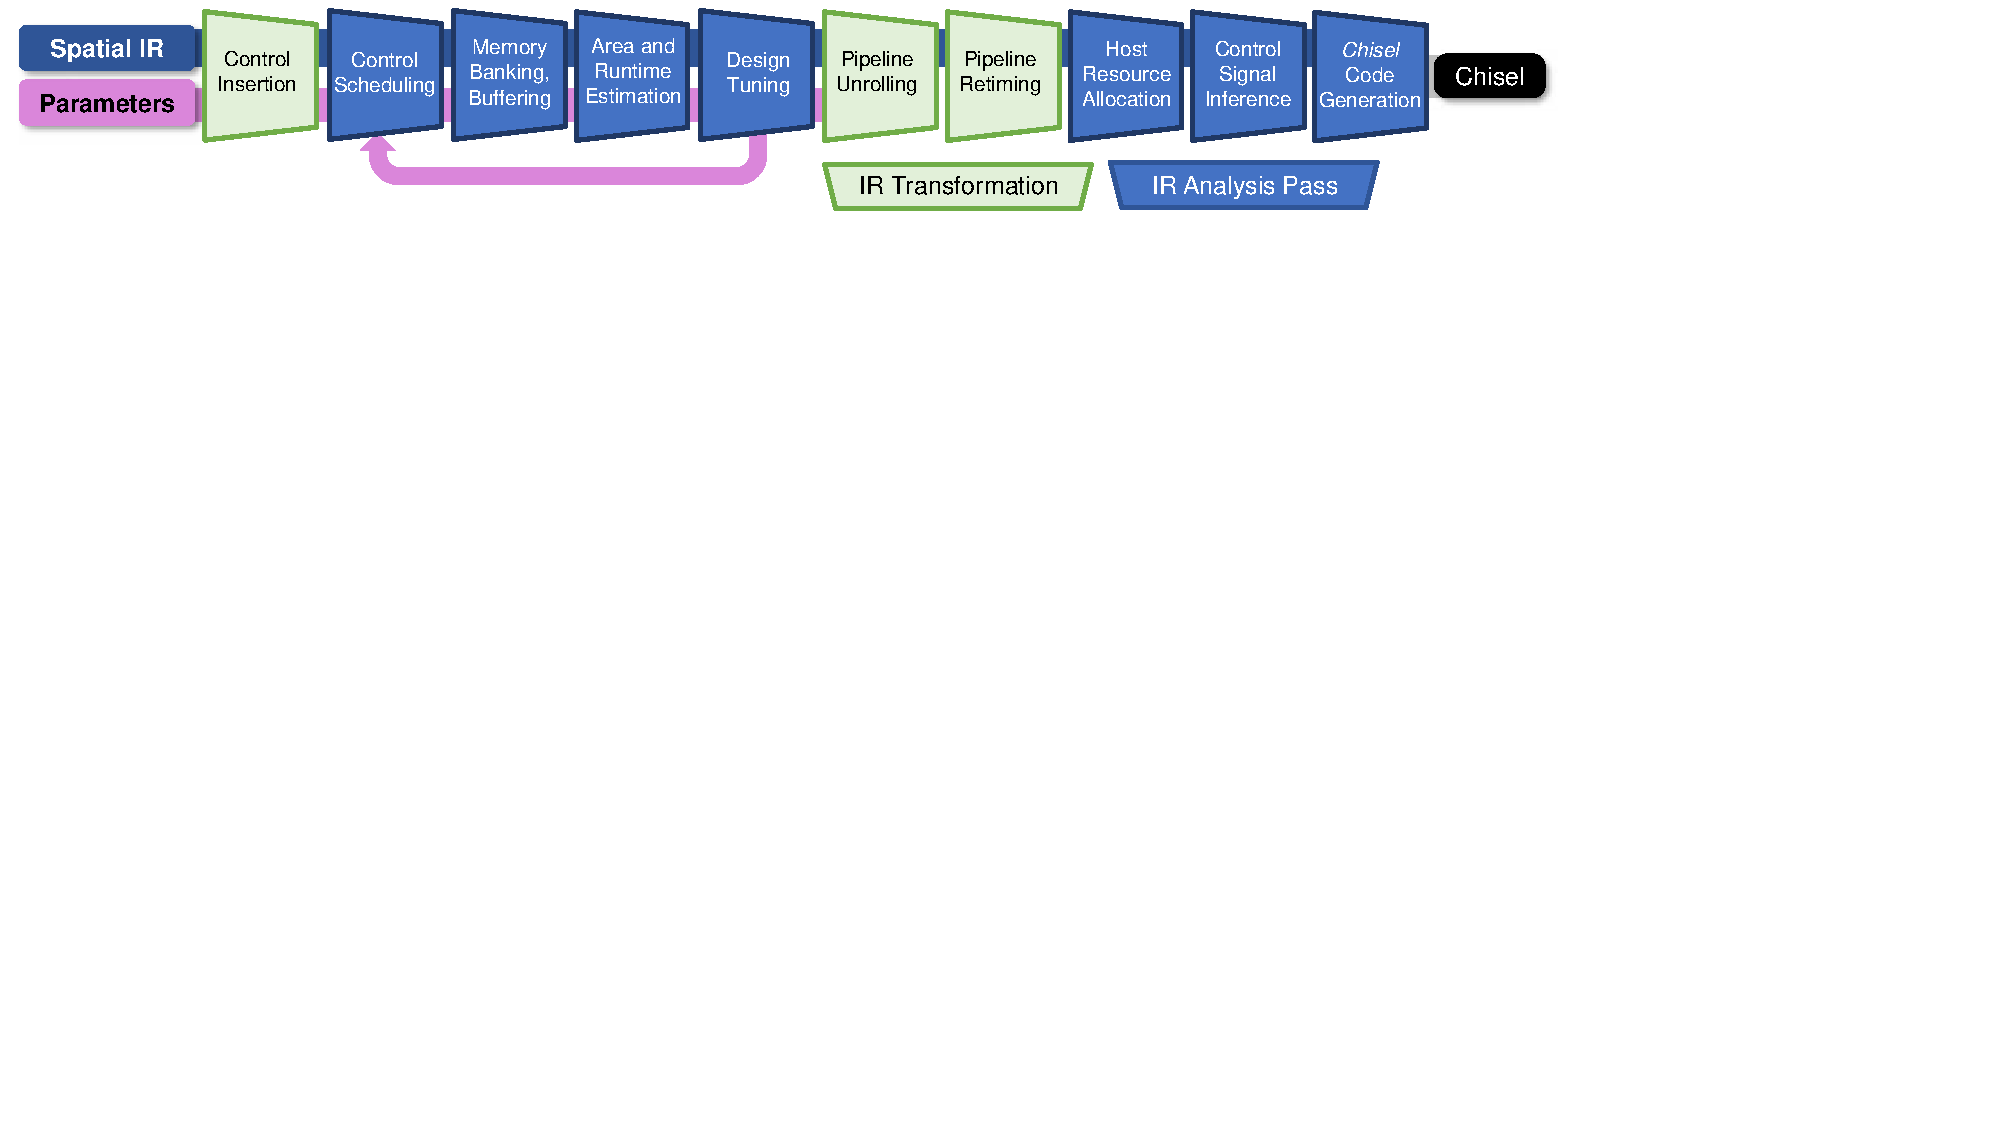
\includegraphics[clip, trim=0.3cm 15.4cm 7.7cm 0.0cm, width=\linewidth]{figs/compiler_flow.pdf}
\caption{A summary of the passes in the Spatial compiler for targeting FPGAs.}
\label{fig:compilerflow}
\end{figure*}


Figure~\ref{fig:sortMerge} shows a simple implementation of a fixed size merge sort in Spatial. Here, data is loaded into on-chip scratchpad, sorted, and then stored back into main memory. 
The language's distinction between on-chip and off-chip memory types makes writing and reasoning about tiled designs like this one much more natural.
This implementation uses a statically sized \texttt{\small{SRAM}} and two \texttt{\small{FIFOs}} to split and order progressively larger size chunks of the local data. 
The chunk size is determined by the outermost loop on line 8, and increments in powers of two. This behavior is best expressed in Spatial as an FSM. 




\section{The Spatial Compiler}
\label{compiler}

The Spatial compiler provides source-to-source translations from applications in the Spatial language to synthesizable hardware descriptions in Chisel RTL~\cite{chisel}. 
In this section, we describe the compiler's intermediate representation and its key passes, as summarized in Figure~\ref{fig:compilerflow}.
Apart from chisel generation, these passes are common to targeting both FPGAs and the Plasticine CGRA. Details of targeting Plasticine are discussed in prior work~\cite{plasticine}.

%For acceleratable code targeted to FPGAs, the output of the compiler is Chisel code \cite{chisel}, roughly the same level of abstraction as Verilog and VHDL.
%The output for CGRAs depends on the requirements of the hardware target, while host (CPU) code is currently generated in C++.
% Spatial is designed to capture algorithms that are intended to run on reconfigurable architectures,
% which gives rise to analyses and optimizations that are not used in software compilers.
% However, information about the target architecture is important to selectively perform a few extra 
% compiler passes and generate the best code for each.  Currently, Spatial can successfully target both FPGAs and a 
% CGRA, Plasticine, and needs to do certain specializations for each with awareness to what the underlying architecture
% looks like.  Here we will briefly discuss what kinds of specializations are done for the two working targets and how the compiler facilitates these passes.


\begin{figure}
%%% trim = left, bottom, right, top
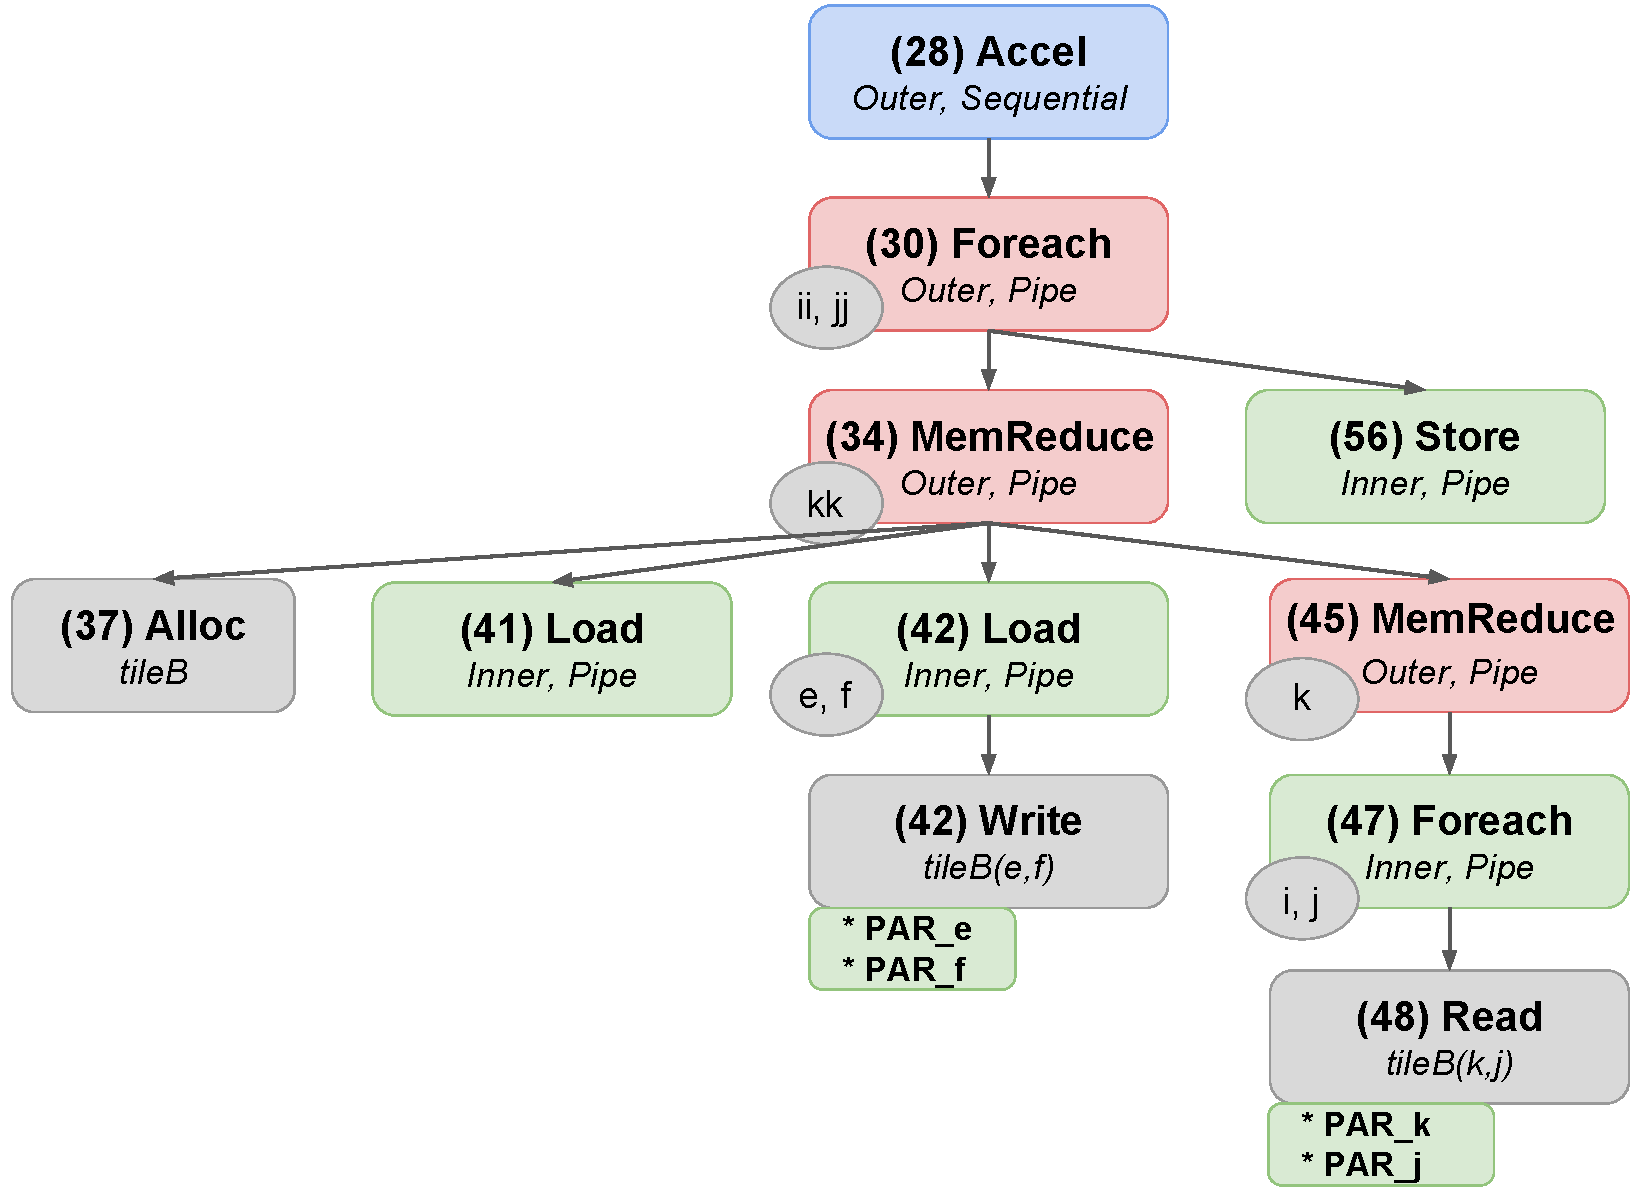
\includegraphics[clip, width=0.9\columnwidth]{figs/control_tree_gemm.pdf}
\vspace{-10pt}
\caption{The control/access tree for the \texttt{\small{SRAM tileB}} in the matrix multiply example in Figure~\ref{fig:matmult}. 
%Control nodes are annotated with their level (outer versus inner), schedule, and loop iterator name. Memory access nodes are annotated with their parallelization factor.
\vspace{-5pt} 
}
\label{fig:controlTree}
\end{figure}

\subsection{Intermediate Representation}

Spatial programs are internally represented in the compiler as a hierarchical dataflow graph (DFG).
Nodes in this graph represent control structures, data operations, and memory allocations, while edges represent data and effect dependencies.
Nesting of controllers directly translates to the hierarchy in the intermediate representation.
Design parameters are kept as graph metadata, such that they can be independently updated without changing the graph itself. 


When discussing DFG transformations and optimizations, it is often useful to think about the graph as a controller/access tree. Figure~\ref{fig:controlTree} shows an example of one such controller tree for the memory {\texttt{\small{tileB}} in the Spatial code example in Figure~\ref{fig:matmult}. Note that transfers between on-chip and off-chip memory expand to a control node which linearly accesses the on-chip memory, in this case by iterators \texttt{e} and \texttt{f}. 
This tree abstracts away most primitive operations, leaving only relevant controller hierarchy and the memory
accesses for a specific memory.


Within the acceleratable subset of Spatial, nodes are formally separated into three categories: 
control nodes, memory allocation nodes, and primitive nodes. 
Control nodes represent state machine structures like \texttt{\small{Foreach}} and \texttt{\small{Reduce}} described in Section~\ref{controls}.
Primitive nodes are operations which may consume, but never produce, control signals, including on-chip memory accesses.
Primitive nodes are further broken down into ``physical'' operations requiring resources and ``ephemeral'' operations which are only used for bookkeeping purposes in the compiler. For example, bit selects and grouping of words into structs require no hardware resources but are used to track necessary wires in the generated code.



% Edit gemm figure here https://docs.google.com/presentation/d/1mScE_E_D2OchZk3xhXiiFQegldOv9iOjSMSic8MITxg/edit?usp=sharing


% The nodes that compose the IR of Spatial provide the handles necessary to do a range of
% hardware optimizations that are specific to spatial architectures.  The combination of
% metadata associated with each node and the hierarchical structure AST that exposes relationships
% between primitives and control structures make it easy to do optimizations on the scheduling of 
% controllers, buffering, banking, and duplication of memory elements, and comprehensive DSE over
% the provided parameter space with low latency.
% \subsection{DRAM Request Consolidation}
% In memory-bound applications, the only way to improve performance is to make better use
% of the available bandwidth.  It is well known that memory bandwidth asymptotically approaches the DRAM's peak bandwidth \todo{is this true?} 
% as the size of each request increases.  This is because of how DRAM pays a penalty for activating and retiring 
% lines of memory cells, and can return more data quickly when consecutive bursts are requested with the same command.

% Unfortunately, there are many applications where the programmer may opt to create logical tensors with 
% relatively small leading dimensions and attempt to load multi-dimensional portions of the structure into on-chip SRAM
% without awareness of how this may thrash the DRAM's controllers in an inefficient way.  For example,
% the programmer may want to solve a multi-objective gradient descent problem that has many training points and very
% few objectives, hence creating a tall and skinny Y matrix.  

% The compiler is able to recognize when the application will be sending out multiple requests to DRAM with
% consecutive addresses, and rewrite the controller to consolidate these into fewer, longer burst commands.
% This means that the user will get fully optimized DRAM requests and physical hardware without needing
% to rethink or change the semantics of the source code. 

\subsection{Control Insertion}

To simplify reasoning about control signals, Spatial requires that control nodes do not contain both physical primitive nodes and other control nodes. The exception to this rule is conditional \texttt{\small{if}} statements, which can be used in the same scope as primitives as long as they contain no control nodes but conditionals themselves.
This requirement is satisfied by a DFG transformation which inserts \texttt{\small{DummyPipe}} control nodes around primitive logic in control bodies which also contain control nodes. The \texttt{\small{DummyPipe}} node is a bookkeeping control structure which is logically equivalent to a loop with exactly one iteration. 
Thereafter, control nodes with primitive nodes are called ``inner'' control nodes, while controllers which contain other nested controllers are called ``outer'' nodes.

% For example, Figure~\ref{fig:matmult} contains some of these nodes. The Foreach in line 32 is an ``outer'' controller, which contains a memory allocation node for tileC 
% (line 33) and another control node, \texttt{\small{MemReduce}} in line 38.  The \texttt{\small{Foreach}} in line 51 is an ``inner'' controller, as it contains
% only primitive nodes generated by the SRAM reads, multiplication, and SRAM store inlined on line 52.


\subsection{Controller Scheduling}
\label{scheduling}
After controller insertion, the compiler will then schedule the operations within each controller.
By default, the compiler will always attempt to pipeline loops regardless of nesting level. 
The behavior of the compiler's scheduler can be overridden by the user using the directives listed in Table~\ref{t:syntaxTable}b.

Inner pipeline schedules are based on their initiation interval. 
The compiler first collects resource initiation intervals for each primitive node in the given controller based on an internal, target-dependent lookup table.
Most primitive operations are pipelined for a resource initiation interval of 1. 
The compiler then calculates all loop carried dependencies within the pipeline based on the dataflow graph.
For non-addressable memories, the total initiation interval is the maximum of path lengths between all dependent reads and the writes. 
For addressable memories, the path length of loop carried dependencies is also multiplied by the difference in write and read addresses.  
If the addresses are loop-independent, the initiation interval is the path length if they may be equal, and 1 if they are provably not equal. If the distance between the addresses cannot be determined statically, the initiation interval is infinite, meaning the loop must be run sequentially.
The total initiation interval is defined as the maximum of the initiation intervals of all loop carried dependencies and all resource initiation intervals. 

The compiler also attempts to pipeline the bodies of outer control nodes in a similar manner, but computes dataflow scheduling in terms of inner control nodes and number of stages rather than primitive nodes and cycles. For example, the outer \texttt{\small{MemReduce}} in line 34 of Figure~\ref{fig:matmult} contains 4 sub-controllers: the load into \texttt{\small{tileA}} (line 41), the load into \texttt{\small{tileB}} (42), the inner \texttt{\small{MemReduce}} (45), and an reduction stage combining intermediate tiles (53). Based on data dependencies, the compiler infers that the two loads can be run in parallel, followed by the inner \texttt{\small{MemReduce}} and the tile reduction. It will also determine that multiple iterations of this outer loop can also be pipelined through these stages.

\subsection{Memory Analysis}
\label{memopts}

Loop parallelization only serves to improve performance if there is sufficient on-chip bandwidth to feed the duplicated computation.
Spatial's memory analysis banks and buffers on-chip memories to maximize this available on-chip read and write bandwidth. 
Memory banking, also called data partitioning, is the process of dividing a memory's address space across multiple physical instances in order to create
additional ports for concurrent accesses within the same controller.
Partitioning is possible when the access patterns are statically predictable and guaranteed to never conflict access the same port/bank. 
While a single port can be time multiplexed, this entirely negates the benefits of parallelization by increasing the whole pipeline's required initiation interval.
Note that while banking can trivially be achieved by memory duplication, Spatial aims to also minimize the total amount of memory resources.  

Spatial leverages the memory partitioning strategy based on conflict polytope emptiness testing described by Wang et. al.~\cite{Wang_banking}. We extend this strategy by accounting for random access patterns and memory accesses across nested loops. Random accesses are modeled as additional dimensions in the conflict polytope as if they were additional loop iterators. Spatial minimizes the number of random access symbols used in this way by identifying affine combinations of random values. For example, an access to a memory at address $x$ and $x+1$ only requires one random variable, $x$, as the second is a predictable, affine function of the first.
Spatial also supports banking per dimension to account for cases where only some dimensions are accessed predictably.

Non-addressed memories like \texttt{\small{FIFOs}} and \texttt{\small{FILOs}} are modeled as addressed memories.
Each access to these memory types is represented as a linear access of all loop iterators around the memory access relative to the memory's definition. Spatial forbids parallelization of outer loops around non-addressed accesses, as this violates the guarantee of equivalent behavior to sequential execution. 

To handle multiple pipelined accesses across stages within an outer loop, Spatial also automatically buffers on-chip memories.
Buffering creates multiple copies of the 
same memory for maintaining versions of the data across overlapped loop iterations. 
Without this optimization, pipeline parallel accesses to the same memory across different stages of a coarse-grain pipeline would not be able to run concurrently.
See Appendix~\ref{banking-appendix} for details on how both banking and buffering are computed.


For example, as shown in Figure~\ref{fig:controlTree}, \texttt{\small{tileB}} has two parallelized accesses, the load on line 42 and the read on line 48. If all (implicit and explicit) parallelization factors are set to 2, this corresponds to 4 accesses per loop. Spatial then builds the access polytope corresponding to all accesses in each loop, and determines the banking strategy that works for both loops. In this example, this means the SRAM will be banked such that each element within a 2x2 square will reside
in a different physical bank to allow fully parallel access. If the \texttt{\small{MemReduce}} on line 34 is pipelined, \texttt{\small{tileB}} will be double buffered to protect the reads (line 48) in one iteration of the outer loop
from the writes (line 42) in the next iteration.

\begin{figure}
\hspace{5pt}
\begin{tabular}{l}
\hline\hline
% function ReachingWrites: 
%   input: $I_w$ $\rightarrow$ set of sets of writes
%   input: $I_r$ $\rightarrow$ set of sets of reads
%   $I'_w$ = $\emptyset$
%   $R$ = Flatten($I_r$)
%   for all $W$ in $I_w$:
%     $W'$ = {$w~\forall~w \in W$ s.t. 
%             $\exists~r \in R$ s.t. MayPrecede($w$,$r$) $\vee~w \cap r \neq \emptyset$}
%     if $W' \neq \emptyset$: add $W'$ to $I'_w$
%   return $I_w'$
% end function

{\begin{lstlisting}[language=Pseudo,linewidth=0.98\columnwidth, mathescape=true]
function GroupAccesses:
   input: $A$ $\rightarrow$ set of reads or writes to $m$
   
   $G$ = $\emptyset$ set of sets of compatible accesses
   
   for all accesses $a$ in $A$:
      for all sets of accesses $g$ in $G$:
       if IComp($a$, $a'$) for all $a'$ in $g$ then
          add $a$ to $g$
          break
       else add {$a$} to $G$
   
   return $G$
end function

function ConfigureMemory:
   input: $A_r$ $\rightarrow$ set of reads of $m$
   input: $A_w$ $\rightarrow$ set of writes to $m$
   
   $G_r$ = GroupAccesses($A_r$)
   $G_w$ = GroupAccesses($A_w$)
   
   $I$ = $\emptyset$ set of memory instances
   
   for all read sets $R$ in $G_r$: 
      $I_r$ = {$R$}
      $I_w$ = ReachingWrites($G_w$, $I_r$)
      $i$ = BankAndBuffer($I_r$, $I_w$)
      for each $inst$ in $I$:
         $I'_r$ = ReadSets[$inst$] + $R$
         $I'_w$ = ReachingWrites($G_w$, $I'_r$)
         if OComp($A_1$,$A_2$) $\forall A_1 \neq A_2 \in (G_w \cup I'_r)$ then:
            $i'$ = BankAndBuffer($I'_r$, $I'_w$)
            if Cost($i'$) < Cost($i$) + Cost($inst$) then:
               remove $inst$ from $I$
               add $i'$ to $I$
               break

      if $i$ has not been merged then add $i$ to $I$ 

   return I
end function
\end{lstlisting}}\\
\hline
\end{tabular}
\vspace{-10pt}
\caption{Banking and buffering algorithm for calculating instances of on-chip memory $m$.
\vspace{-10pt}
}
\label{fig:bank_alg}
\end{figure}

Figure~\ref{fig:bank_alg} gives pseudocode for Spatial's algorithm to bank and buffer accesses to a given memory \emph{m} across loop nests. For each access $a$ to $m$, we first define an iteration domain $D$ for that access. This domain is the multi-dimensional space of possible values of all loop iterators for all loops which contain $a$ but which do not contain $m$. 

We then group read and write accesses on $m$ into ``compatible'' sets which occur in parallel to the same physical port but which can be banked together (lines 1 -- 14). 
Two accesses $a_1$ and $a_2$ within iteration domains $D_1$ and $D_2$
are banking compatible ($IComp$) if
\[ IComp(a_1,a_2) = \nexists~\vec{i} \in (D_1 \cup D_2) ~s.t.~a_1(\vec{i}) = r_2(\vec{i}) \]
where $a(i)$ is the multi-dimensional address corresponding to access $a$ for some vector of iterator values $i$.
This check can be implemented using a polytope emptiness test.

After grouping, each group could be directly mapped to a coherent ``instance'', or copy, of $m$. 
However, this approach would typically use more resources than required. To minimize the total number of memory instances, we next greedily merge groups together (lines 25 -- 39). Merging is done when the cost of a merged instance is less than the cost of adding a separate, coherent instance for that group.
Two sets of accesses $A_1$ and $A_2$ allow merging ($OComp$) if 
\[ OComp(A_1, A_2) = \nexists~ (a_1 \in A_1, a_2 \in A_2) ~s.t. \]
\[  LCA(a_1, a_2) \in Parallel \cup (Pipe \cap Inner) \]
where \emph{Parallel}, \emph{Pipe}, and \emph{Inner} are the set of Parallel, pipelined, and inner controllers in the program, respectively.
If this condition holds, all accesses between the two instances either occur sequentially or occur as part of a coarse-grain pipeline. Sequential accesses can be time multiplexed, while pipelined accesses are buffered.

\emph{ReachingWrites} returns all writes in each set which may be visible to any read in the given sets of reads. Visibility is possible if the write may be executed before the read and may have an overlapping address space.

The \emph{BankAndBuffer} function produces a single memory instance from memory reads and writes.
Here, each set of accesses is a set of parallel reads or writes to a single port of the memory instance.
Accesses in different sets are guaranteed not to occur to the same port at the same time.
Therefore, a common banking strategy is found which has no bank conflicts for any set of accesses. 
This banking strategy is found using iterative polytope emptiness testing as described by Wang et. al.~\cite{Wang_banking}. 
A separate emptiness test is run for each set of parallel accesses for each proposed strategy.

The required buffer depth \emph{d} for a pair of accesses $a_1$ and $a_2$ to $m$ is computed as
\[
d(a_1, a_2) = \left\{\begin{matrix} 1 & LCA(a_1, a_2) \in Seq \cup Stream \\ dist(a_1,a_2) & LCA(a_1,a_2) \in Pipe \end{matrix}\right.
\]
where \emph{dist} is the minimum of the depth of the LCA and the dataflow distance of the two direct children of the LCA which contain $a_1$ and $a_2$. \emph{Seq}, \emph{Stream}, and \emph{Pipe} are the set of sequential, streaming, and pipelined controllers, respectively. Buffering addressable memories across streaming accesses is currently unsupported.
The depth of a set of reads $R$ and writes $W$ is then
\[ Depth(R,W) = max\{ d(w,a)~\forall ~(w,a) \in W \times (W\cup R) \} \]

The port of each access within a buffer is determined from the relative distances between all buffered accesses.
Spatial requires that no more than one coarse-grained controller or streaming controller is part of a merged instance.
The final output of the greedy search is a set of required physical memory instances for memory \emph{m}.



\section{Area and Runtime Estimation}
\label{sec:modeling}
%\gist{Characterize DHDL templates and construct models estimate area and runtime in terms of cycle count.
%Estimation must account for effects from low-level tool optimizations. This drives a DSE loop}
In this section, we describe our modeling methodology. Our models account for the various
design parameters for each DHDL template, as listed in Table~\ref{t-hwtemplates}, as well as optimizations done by low-level logic
synthesis tools in order to accurately estimate resource usage.

\subsection{Modeling Considerations}
\label{ss:modeling-con}
%\gist{Low-level tools do fancy optimizations which estimator should be aware of.
%  Examples: LUT packing, logic duplication, using BRAMs for large delay lines,
%unavailable LUTs etc. Also, certain device architecture features play a significant role}
The resource requirements of a given application implemented on an FPGA depend both on the target device and on the toolchain.
Heterogeneity in the FPGA fabric, use of FPGA resources for routing, and other low-level optimizations performed by logic
synthesis tools often have a significant impact on the total resource consumption of a design. Since these factors reflect
the physical layout of computation on the device after placement and routing, they are not captured directly in the application's dataflow graph.
We identify and account for the following factors:
%\begin{itemize}

\paragraph{LUT and register packing} Basic compute units in FPGAs are typically composed of a lookup table (LUT), and a small number of single bit multiplexers, registers, and full adders.
  Modern FPGA LUTs support up to 8-input binary functions but are often implemented using a pair of smaller LUTs~\cite{stratixv,virtex7}.
  When these LUTs can be configured and used independently, vendor placement tools attempt to ``pack'' multiple small functions into a single 8-input unit.
  LUT packing can have a significant impact on design resource requirements.
  In our experiments, we are able to pack about 80\% of the functions in each design in pairs, decreasing the number of used LUTs by about 40\%.

\paragraph{Routing Resources} Logic synthesis tools require a significant amount of resources to establish static routing connections
between two design points (e.g., a multiplier and a block RAM) which fit in the path's clock period. While FPGAs have dedicated routing resources,
logic synthesis tools may have the option to use LUTs for routing. These LUTs may then be unavailable to be used for ``real'' compute.
In our designs, ``route-through'' LUTs typically account for about 10\% of the total number of used LUTs.


\paragraph{Logic duplication} Logic synthesis tools often duplicate resources such as block RAMs
and registers to avoid routing congestion and to decrease fan out. While duplicated registers typically
encompass around 5\% of the total number of registers required in our designs, we found that block RAM
duplication can increase RAM utilization by 10 to 100\%, depending on the complexity of the design.


\paragraph{Unavailable resources} FPGA resources are typically organized in a hierarchy, such as Altera's Logic Array Block structure (10 LUTs)
and Xilinx's Slice structure (4 LUTs). Such organizations impose mapping constraints which can lead to
resources that are rendered unusable. In our experiments, the number of unusable LUTs made up only about 4\% of the design's total LUT usage.
%\end{itemize}
%\todo{Need to figure out how to say this.} We focus on one Altera device in this paper, the Stratix V.
%ALMs in the Stratix V have 4 registers. We experimentally found that in most designs, just over 50 percent
%of the registers in each ALM is used. Thus, we use a simple model where we assume registers do not
%contribute to the ALM count unless they number over 2x the number of ALMs used to implement logic.
%(packed lut count) + max(0, regs/2 - (packed lut count))

\subsection{Methodology}
In order to model runtime and resource requirements of DHDL designs, we first need an estimate of the area requirements and
propagation delay of every DHDL template. Area requirements include the number of digital signal processing
units (DSPs), device block RAMs, LUTs, and registers that each template requires. To facilitate LUT packing estimation,
we split template LUT resource requirements into the number of ``packable'' and ``unpackable'' LUTs required.
%For templates with documented implementations such as floating point operations \cite{fp-altera}, we gather resource and cycle data in part by summarizing IP core documentation. However, these user manuals typically do not give resource usage breakdowns at the binary function level.
We obtain characterization data by synthesizing multiple instances of each template instantiated for combinations of its parameters as given in Table~\ref{t-hwtemplates}.
%Our model assumes that all primitive multi-cycle nodes (such as multiply) are fully pipelined.
Using this data, we create analytical models of each DHDL template's resource requirements and cycle counts for
a predefined fabric clock. The area and cycle count of controller templates are modeled as functions of the latencies of the nodes contained within them.
The total cycle count for a \emph{MetaPipe}, for example, is modeled using the recursive function
\begin{displaymath}
(N-1)\max(cycles(n) | n \in nodes) + \sum_{n \in nodes} cycles(n)
\end{displaymath}
where \emph{N} is the number of iterations of the \emph{MetaPipe} and \emph{nodes} is the set of nodes contained in the \emph{MetaPipe}.

Most templates require about six synthesized designs to characterize their resource and area usage as a function of their parameters. Note that these models include estimates of off-chip memory access latency as a function of the
number and length of memory commands, as well as contention due to competing accessors. Since template models are application-independent, each needs only be characterized once for a given target device and logic synthesis toolchain. The synthesis times required to model templates can therefore be amortized over many applications.
%We show a subset of the template models used in our experiments in Table~\ref{table:benchmarks}.
%\note{not sure I understand this. Which part is app-independent. Presumably the way to explore the space will dependt on the application. Is this only for the device models? }

Using these models, we run a pair of analysis passes over the application's DHDL intermediate representation to estimate design cycle counts and area requirements.

%\begin{table*}
%\centering\footnotesize
%\begin{tabular}{m{1.7cm}c{4.7cm}c{4.7cm}m{4.5cm}}
%\toprule
%{\bf Node} & {\bf Cycle Count} & {\bf Area} & {\bf Parameters} \\ \midrule
%TileLd &  & & \\ \midrule
%TileSt &  & & \\ \midrule
%Sequential &  & & \\ \midrule
%Parallel &
%  \begin{lstlisting}[mathescape=true, numbers=none, language=DHDL]
%    Cycles[body] + N * Cycles[accum]
%  \end{lstlisting}
%   & Area[body] & \texttt{accum}: accumulation loop for reductions \\ \midrule
%CoarsePipe & & & \\ \midrule
%Pipe &  & &  \\ \midrule
%BRAM & 0 & & \\ \midrule
%Priority Queue & 0 & & \\ \midrule
%Reg & 1 & & \\ \bottomrule
%\end{tabular}
%\caption{Area and cycle count models for DHDL nodes. Note that \emph{BRAM} and \emph{Priority Queue} have no associated cycle counts %as this is accounted for entirely by \emph{Ld} and \emph{St} templates.}
%\label{table:benchmarks}
%\end{table*}

\subsubsection{Cycle Count Estimation}
In the first analysis pass, we estimate the total runtime of the design on the FPGA.
Since the DHDL intermediate representation is hierarchical in nature, this pass is done recursively.
The total runtime of \emph{MetaPipe} and \emph{Sequential} nodes is calculated first by determining
the runtime of all controller nodes contained within them. The total propagation delay of a single
iteration of a \emph{Pipe} is the length of the body's critical path, calculated using a depth first
search of the body's subgraph and the propagation delay of all primitive nodes within the graph.
Input dataset sizes, given as user annotations in the high-level program, are used by the analysis pass
along with tiling factors to determine the iteration counts for each controller template.
Iteration counts are then used to calculate the total runtime of the respective controller nodes. %using the equations given in Table~\ref{table:benchmarks}.


\subsubsection{Area Estimation}
Since the FPGA resource utilization of a design is sensitive to factors that are not directly captured
in the design's dataflow graph, we adopt a hybrid approach in our area analysis.

We first estimate the area of the DHDL design by counting the resource
requirements of each node using their pre-characterized area models. In \emph{Pipe} bodies, we also
estimate the resources required for delaying signals. This is done by recursively calculating the
propagation delay of every path to each node using depth first search. Paths with slack relative to
the critical path to that node require their width (in bits) multiplied by the slack delay resources.
Delays over a synthesis tool-specific threshold are modeled as block RAMs.
Otherwise, they are modeled as registers. Note that this estimation assumes ASAP scheduling.

We model LUT routing usage, register duplication, and unavailable LUTs using a set of small artificial
neural networks implemented using the Encog machine learning library~\cite{encog}.
Each network has three fully connected layers with eleven input nodes, six hidden layer nodes, and a single output node. We chose to use
three layer neural networks as they have been proven to be capable of fitting a wide number of function classes with arbitrary precision, including polynomial functions of any order~\cite{science}.
One network is trained
for each factor on a common set of 200 design samples with varying levels of resource usage to give a representative sampling of the space. Choosing the correct
network parameters to obtain the lowest model error is typically challenging, but in our experiments we found that above four nodes in the hidden layer,
the exact number of hidden layer nodes made little difference.
Duplicated block RAMs are estimated as a linear function of the number of routing LUTs, as we found that this gave the best estimate of design routing complexity in practice. This linear function was fit using the same data used to train the neural networks. Like the template models, these neural networks are application independent and only need to be trained once for a given target device and toolchain.

We use the raw resource counts as an input to each of our neural networks to obtain global estimates for routing LUTs,
duplicated registers, and unavailable LUTs. We estimate the number of duplicated block RAMs using the routing LUTs.
These estimates are then added to the raw resource counts to obtain a pre-packing resource estimate. For the purposes
of LUT packing, we assume routing LUTs are always packable.

Lastly, we model LUT packing using the simple assumption that all packable LUTs will be packed. The target device
in our experiments supports pairwise LUT packing, so we estimate the number of compute units used for logic as
the number of unpackable LUTs plus the number of packable LUTs divided by two. We assume that each compute unit
will use two registers on average. We model any registers unaccounted for by logic compute units as requiring
compute units with two registers each. This gives us the final estimation for LUTs, DSPs, and BRAM.

%To account for resources utilized by nodes in the dataflow graph, we then perform a detailed characterization of all primitive nodes
%in DHDL and use the data to count the resources required to implement the datapath.

%We use a simple model for LUT packing, where we assume that pairs of LUTs which
%can be packed are packed.
%Table \todo{Table with control, memory, and mem generator templates as functions + description of what each variable is - should have four columns(?): node name, area function, and cycle function, and variable description?} gives examples of the resource usage and cycle latency of memory, controller, and memory command generator templates as functions of their respective parameters.
%We model each of the factors listed in section~\ref{ss:modeling-con} using a two layer artificial neural networks

%We use the Encog machine learning library~\cite{encog} to implement our neural network.

\subsection{Design space exploration}
%\gist{We explore this list (have a list somewhere) of design points
%  for each benchmark. Input dataset size is considered during DSE
%as it impacts the search space. We perform simple optimizations
%to prune search space to discount invalid combinations and designs
%which will not fit in the given amount of resources}
Our design space exploration tool uses the resource and cycle count estimates
to explore the space of designs described by the parameters in Table~\ref{t-hwtemplates}.
As we are dealing with large design spaces on the order of millions of points even for small benchmarks,
we prune invalid and suboptimal points in the search space using a few simple heuristics:
\begin{itemize}
  \item Parallelization factors considered are integer divisors of the respective iteration counts. We use this pruning strategy because non-divisor factors create edge cases which require additional modulus operations. These operations can significantly increase the latency and area of address calculation, typically making them poor design parameter choices \cite{raghus-paper}.
  \item Tile sizes considered are divisors of the dimensions of the annotated data size. Similar to parallelization factors, tile sizes with edge cases are usually suboptimal as they increase load and store area and latency with additional indexing logic.
  \item Automatic banking of on-chip memories eliminates the memory banks as an independent variable. This prunes a large set of suboptimal design points where on-chip memory bandwidth requirements do not match the amount of parallelization.
  \item The total size of each local memory is limited to a fixed maximum value.
  %\item Design points that have larger parameter sizes than a previously estimated point
  %  are pruned if the previously estimated point does not fit in the given FPGA resources.
\end{itemize}

These heuristics defines a ``legal'' subspace of the total design space. In our experiments, we randomly generate estimates for up to $75,000$ legal points to give a representative view of the entire design space. We immediately discard illegal points.

% ------------------ ALREADY COMMENTED -------------------------
%Using the DHDL templates described in the previous section, we estimate total FPGA resource usage and runtime. Our estimates are made using a set of models at the template and design level. While creating these models requires a set of pre-characterization hardware synthesis runs, this characterization is application-independent and need only be run once for a given target device.

%Creating these models requires a set of pre-characterization hardware synthesis runs, but benchmarks used for characterization tend to be much smaller, and hence synthesize faster, than any real application. More importantly, characterization is application-independent and need only be run once for a given target FPGA.

%Template area and cycle models are based on simple, individual characterizations.
% --------------------------------------------------------------

% ---------------------- ALREADY COMMENTED ------------------------------------
%\begin{itemize}
%\item Template area and cycle count based on individual characterization (include table for controllers?)
%\item ALM packing based on rough estimate
%\item Simple ASAP schedule estimation for adding delay registers along combinational paths
%\item Routing for ALMs and regs based on neural network model, as is unavailable ALM model
%\item Routing BRAMs?
%\end{itemize}
% -----------------------------------------------------------




% ---------------------- ALREADY COMMENTED ------------------------------------
%Characterization and modeling is device-specific but application-independent.
%Once created, each model can be used across many different applications on the same


%Even a relatively small number of parameters can lead to large design spaces. If hardware place and route pass is used for evaluation, each
%Naively implemen automated design space acceleration of application-specific accelerators is quite time consuming, both because of the size of space and the length of time

%Modern FPGAs include





\subsection{Design Space Exploration}
\label{dse}
The scheduling and memory banking options identified by the compiler, together with loop parallelization and tile size parameters, forms a design space for the application. 
The design tuning pass is an optional compiler pass which allows for fast exploration of this design space in order to make area/runtime design tradeoffs.
When design tuning is enabled, it repeatedly picks design points and evaluates them by rerunning the control scheduling, memory analysis, and estimation analysis passes. The output from this search is a single set of parameters from the Pareto frontier.


%By exposing parameters to the compiler it is possible to automatically perform
%design space exploration on the source code. 
%The code generated will result optimized for speed and logic utilization. 
Unfortunately, application design spaces tend to be extremely large, and exhaustive search on an entire space is often infeasible. Of the benchmarks discussed in Section~\ref{evaluation}, 
only BlackScholes has a relatively small space of about $80,000$ points. While this space can be explored exhaustively by Spatial in a few minutes, other spaces are much larger, spanning $10^6$ to $10^{10}$ points and
taking hours or days to exhaustively search. For example, even with the few explicit design parameters exposed in the code in Figure~\ref{fig:matmult}, when combined with implicit pipelining and parallelization parameters, this code already has about $2.6\times10^8$ potential designs.
DHDL~\cite{dhdl} employed random search after heuristic pruning, reducing the total space by two to three orders of magnitude. However, this approach has high variance on larger design spaces and may inadvertently prune desirable points.

To reduce the variance on larger design spaces, Spatial's design space exploration flow integrates an active learning-based autotuner called HyperMapper~\cite{Bodin2016:PACT16,NardiBSVDK17,Saeedi_ICRA_2017}.
HyperMapper is a multi-objective derivative-free optimizer (DFO), and has already been demonstrated on the SLAMBench benchmarking framework \cite{nardi2015introducing}. 
HyperMapper creates a surrogate model using a Random Forest regressor, and predicts the performance over the parameter space. This regressor is initially built using only few hundred random design point samples and is iteratively refined in subsequent active learning steps.


\subsection{Unrolling}
Following selection of values for design parameters, Spatial finalizes these parameters in a single graph transformation which unrolls loops and duplicates memories as determined by prior analysis passes. 
\texttt{Reduce} and \texttt{MemReduce} patterns are also lowered into their imperative implementations, with hardware reduction trees instantiated from the given reduction function. 
The two \texttt{MemReduce} loops in Figure~\ref{fig:matmult}, for example, will each be lowered into unrolled \texttt{Foreach} loops with explicitly banked memory accesses and explicitly duplicated multiply operations. The corresponding reduction across tiles (lines 52~--~53) are lowered into a second stage of the \texttt{Foreach} with explicit reduction trees matching the loop parallelization. 

\subsection{Retiming}
After unrolling, the compiler retimes each inner pipeline to make sure data and control signals properly line up and ensure that the target clock frequency can be met.
To do this, the compiler orders primitive operations within each pipeline based on effect and dataflow order.
This ordering is calculated using a reverse depth first search along data and effect dependencies. 
A second forward depth first search is then used to minimize delays in reduction cycles.
Based on this ordering, the compiler then inserts pipeline and delay line registers based on lookup tables which map each primitive node to an associated latency. Dependent nodes which have less than a full cycle of delay are kept as combinational operations, with a register only being inserted after the last operation.
This register insertion maximizes the achievable clock frequency for this controller while also minimizing the required initiation interval.



\begin{table*}

\fontsize{8}{9}\selectfont
\begin{tabular}{m{36pt} m{56pt} m{32pt} l d{3.0} d{6.0} d{4.0} d{4.0} d{4.1} }
\ml{}                                                           & \ml{}           &\ml{}          & \ml{}                & \mc{LOC}    & \mc{LUTs}         & \mc{BRAM}         & \mc{DSPs}         & \mc{Time (ms)} \\ \toprule
\ml{Benchmark}                                                  & \ml{Data Sizes} &\ml{DSE size}  & \ml{\emph{Capacity}} & \mc{---}    & 914400            & 1680              & 5640              & \mc{---} \\
\midrule

% \multirow{3}{*}{
% \hspace{-8pt}\begin{tabular}{l}
% \bf{AES} \\
% Encryption \\
% \end{tabular}
% }                                                               &
% \multirow{3}{*}{32kB data }
%                                                                 & SDAccel         & 333                  & 338305      & 589               & 0                 & 2.23 \\
%                                                                 &                 & Spatial              & 150         & 600027            & 442               & 9                 & 14.45 \\
%                                                                 &                 & \ml{Relative}        & \mc{54.8\%} & \mc{0.56$\times$} & \mc{1.33$\times$} & \mc{1.33$\times$} & \mc{0.15$\times$} \\ \midrule

\multirow{3}{*}{
\hspace{-8pt}\begin{tabular}{l}
\bf{BS} \\
Black-Scholes \\
option pricing \\
\end{tabular}
}                                                               &
\multirow{3}{*}{ 960,000 options }
& \multirow{3}{*}{ $7.7\times 10^4$ }
                                                                & SDAccel         & 175   & 363368      & 550  & 290 & 6.18 \\
                                              &&                & Spatial         & 93    & 698885      & 493  & 945 & 3.79 \\
                                              &                 &                 & \ml{Improv.} & \mc{46.8\%} & \mc{0.52$\times$} & \mc{1.12$\times$} & \mc{0.31$\times$} & \mc{1.63$\times$} \\ \midrule

\multirow{3}{*}{
\hspace{-8pt}\begin{tabular}{l}
\bf{GDA} \\
Gaussian \\
discrimination \\
\end{tabular}
}                                                               &
\multirow{3}{*}{
\hspace{-8pt}\begin{tabular}{l}
1024 rows \\
96 dimensions \\
\end{tabular}
} & \multirow{3}{*}{ $3.0\times 10^{10}$ }
                                                                & SDAccel          & 73    & 356857      & 594   & 108   & 10.75 \\
                                              &&                 & Spatial          & 64    & 378130      & 858   & 216   & 1.27  \\
                                              &&                 & \ml{Improv.} & \mc{12.3\%} & \mc{0.94$\times$} & \mc{0.69$\times$} & \mc{0.50$\times$} & \mc{8.48$\times$} \\ \midrule


\multirow{3}{*}{
\hspace{-8pt}\begin{tabular}{l}
\bf{GEMM} \\
Matrix \\
multiply \\
\end{tabular}
}                                                               &
\multirow{3}{*}{
\hspace{-8pt}\begin{tabular}{l}
A: 1024$\times$1024 \\
B: 1024$\times$1024 \\
\end{tabular}
}
& \multirow{3}{*}{ $2.6\times 10^8$ }
                                                                & SDAccel          & 110         & 341894            & 674               & 206                & 1207.26 \\
                                              &&                 & Spatial          & 44          & 426295            & 500               & 798               & 878.45 \\
                                              &&                 & \ml{Improv.} & \mc{60.0\%} & \mc{0.80$\times$} & \mc{1.35$\times$} & \mc{0.26$\times$} & \mc{1.37$\times$} \\ \midrule


\multirow{3}{*}{
\hspace{-8pt}\begin{tabular}{l}
\bf{KMeans} \\
K-Means \\
clustering\\
\end{tabular}
}                                                               &
\multirow{3}{*}{
\hspace{-8pt}\begin{tabular}{l}
200 iterations \\
320$\times$32 points \\
\end{tabular}
}
& \multirow{3}{*}{ $2.1\times 10^6$ }
                                                                & SDAccel          & 146         & 356382            & 657               & 539               & 73.04 \\
                                              &&                 & Spatial          & 81          & 369348            & 453               & 105                & 53.25 \\
                                              &&                 & \ml{Improv.} & \mc{44.5\%} & \mc{0.96$\times$} & \mc{1.45$\times$} & \mc{5.13$\times$} & \mc{1.37$\times$} \\ \midrule




\multirow{3}{*}{
\hspace{-8pt}\begin{tabular}{l}
\bf{PageRank} \\
Node ranking \\
\end{tabular}
}                                                               &
\multirow{3}{*}{
\hspace{-8pt}\begin{tabular}{l}
DIMACS10 \\
Chesapeake \\
10000 iterations \\
\end{tabular}
}
& \multirow{3}{*}{ $4.1\times 10^3$ }
                                                                & SDAccel          & 112         & 337102            & 549               & 17                & 2041.62 \\
                                              &&                 & Spatial          & 77          & 418128            & 862               & 81                & 587.35 \\
                                              &&                 & \ml{Improv.} & \mc{31.2\%} & \mc{0.81$\times$} & \mc{0.64$\times$} & \mc{0.21$\times$} & \mc{3.48$\times$} \\ \midrule


% \multirow{3}{*}{
% \hspace{-8pt}\begin{tabular}{l}
% \bf{Sobel} \\
% Image edge detection \\
% \end{tabular}
% }                                                               &
% \multirow{3}{*}{512$\times$512 bmp}
%                                                                & SDAccel         & 90                   & 341100      & 560               & 0                 & 0.19 \\
%                                                                &                 & Spatial              & 50          & 514885            & 574               & 177               & 20.74 \\
%                                                                &                 & \ml{Improv.}        & \mc{44.4\%} & \mc{0.66$\times$} & \mc{0.98$\times$} & \mc{0.07$\times$} & \mc{0.01$\times$} \\ \midrule

\multirow{3}{*}{
\hspace{-8pt}\begin{tabular}{l}
\bf{SW} \\
DNA \\
alignment \\
\end{tabular}
}                                                               &
\multirow{3}{*}{256 base pairs}
& \multirow{3}{*}{ $2.1\times 10^6$ }
                                                                & SDAccel           & 240         & 541617            & 547               & 12                & 8.67 \\
                                              &&                 & Spatial           & 82          & 330063            & 470               & 9                 & 0.61 \\
                                              &&                 & \ml{Improv.}  & \mc{65.8\%} & \mc{1.64$\times$} & \mc{1.16$\times$} & \mc{1.33$\times$} & \mc{14.15$\times$} \\ \midrule


\multirow{3}{*}{
\hspace{-8pt}\begin{tabular}{l}
\bf{TQ6} \\
TPC-H Q6 \\
\end{tabular}
}                                                               &
\multirow{3}{*}{6,400,000 records}
& \multirow{3}{*}{ $3.5\times 10^9$ }
                                                                & SDAccel          & 74          & 356978            & 548               & 15                & 18.61 \\
                                              &&                 & Spatial          & 48          & 472868            & 574               & 393               & 13.97 \\
                                              &&                 & \ml{Improv.} & \mc{35.1\%} & \mc{0.75$\times$} & \mc{0.95$\times$} & \mc{0.04$\times$} & \mc{1.33$\times$} \\


\midrule
\ml{Average}                                  &&                 & \ml{Improv.} & \mc{42.3\%} & \mc{0.87$\times$} & \mc{1.01$\times$} & \mc{0.42$\times$} & \mc{2.90$  \times$} \\

\bottomrule
\end{tabular}

\caption{Number of lines of code (LOC), area utilization, and runtime comparisons between SDAccel and Spatial on a single VU9P FPGA.
For reference, the first row lists the total number of FPGA resources available. LOC improvements are percent improvements from SDAccel. The remaining improvement factors are calculated as $(SDAccel / Spatial)$.}
\label{t:hls_comp}
\end{table*}


\subsection{Code Generation}
Prior to code generation, the compiler first allocates register names for every \texttt{\small{ArgIn}}, \texttt{\small{ArgOut}}, and \texttt{\small{HostIO}}.
In the final pass over the IR, the code generator then instantiates hardware modules from a library of custom, parameterized RTL templates written in Chisel and infers and generates the logic required to stitch them together.  These templates include state machines that manage communication between the various control structures and primitives in the application, as well as the banked and buffered memory structures and efficient arithmetic operations.  Finally, all generated hardware is wrapped in a target-specific, parameterized Chisel module that arbitrates off-chip accesses from the accelerator with the peripheral devices on the target FPGA. 


\section{Evaluation}
\label{evaluation}

In this section, we evaluate Spatial by comparing programmer productivity and the performance of generated designs to Xilinx's commercial HLS tool, SDAccel. We then evaluate the HyperMapper design tuning approach and demonstrate Spatial's advantages for portability across FPGAs and the Plasticine CGRA.

\subsection{FPGA Performance and Productivity}
We first evaluate the FPGA performance and productivity benefits of Spatial against SDAccel, a commercial C-based programming tool from Xilinx for creating high-performance accelerator designs. We use SDAccel in our study as it has similar performance and productivity goals as Spatial, supports the popular OpenCL programming model, and performs several optimizations related to loop pipelining, unrolling, and memory partitioning~\cite{sdaccel}. Baseline implementations of the benchmarks in Table~\ref{t:hls_comp} have been either obtained from a public SDAccel benchmark suite from Xilinx~\cite{sdaccelBench}, or written by hand. Each baseline has then been manually tuned by using appropriate HLS pragmas~\cite{hlsPragmaRef} to pick loop pipelining, unrolling, and array banking factors, and to enable dataflow optimizations. Design points for Spatial are chosen using the DSE flow described in Section~\ref{dse}.

We measure productivity by comparing number of lines of source code used to describe the FPGA kernel, excluding host code. We measure performance by comparing runtimes and FPGA resources utilized for each benchmark on a Xilinx Ultrascale+ VU9P board with a fabric clock of 125 MHz, hosted on an Amazon EC2 F1 instance. We generate FPGA bitstreams targeting the VU9P architecture for each benchmark using both Spatial and SDAccel, and obtain resource utilization data from the post place-and-route reports. We then run and verify both designs on the FPGA and measure the execution times on the board. CPU setup code and data transfer time between CPU and FPGA is excluded from runtime measurements for both tools.

Table~\ref{t:hls_comp} shows the input dataset sizes and the full comparison between lines of source code, resource utilization, and runtime of the benchmarks implemented in SDAccel and Spatial.
In terms of productivity, language constructs in Spatial like \texttt{\small{load}} and \texttt{\small{store}} for transferring dense sparse data from DRAM reduces code bloat and increases readability.
Furthermore, by implicitly
inferring parameters such as parallelization factors and loop initiation intervals, Spatial code is largely free of annotations and pragmas.

Spatial achieves speedups over SDAccel of $1.63\times$ and $1.33\times$ respectively on \emph{BlackScholes} and \emph{TPC-H Q6}. Both benchmarks
stream data from DRAM through a deeply pipelined datapath which is amenable to FPGA acceleration. Dataflow support in SDAccel using the DATAFLOW pragma~\cite{dataflowRef} and streaming support in Spatial allows both tools to efficiently accelerate such workloads. In \emph{K-Means}, coarse-grained pipelining support allows Spatial to achieve roughly the same performance as SDAccel using $1.5\times$ fewer BRAMs.
Specialized DRAM scatter/gather support enables Spatial to achieve a $3.48\times$ speedup on \emph{PageRank}.

We see speedups of $8.48\times$, $1.37\times$, and $14.15\times$ for compute-heavy workloads \emph{GDA}, \emph{GEMM}, and \emph{SW}, respectively. The baseline for \emph{SW} is implemented by Xilinx as a systolic array, while the Spatial implementation uses nested controllers. \emph{GEMM} and \emph{GDA} contain opportunities for coarse-grained pipelining that are exploited within Spatial. 
GDA, for example, contains an outer product operation, during which the data in the same buffer is repeatedly accessed and reused. While this operation can be pipelined with a preceding loop producing the array, SDAccel's DATAFLOW pragma does not support such access patterns that involve reuse. As a result, SDAccel requires larger array partitioning and loop unrolling factors to offset the performance impact, at the expense of consuming more FPGA BRAM.
In addition, nested controllers in \emph{GEMM}
can be parallelized and pipelined independently in Spatial, while SDAccel automatically unrolls all inner loops if an outer loop is parallelized. Spatial can therefore explore
design points that cannot be easily expressed in SDAccel. Finally, as the Spatial compiler performs analyses on a parameterized IR, the compiler can reason about larger parallelization factors without expanding the IR graph.
SDAccel unrolls the graph as a preprocessing step, hence creating larger graphs when unrolling and array partitioning factors are large.
This has a significant impact on the compiler's memory footprint and compilation times, making better designs difficult or impossible to find.

Spatial provides a productive platform to program FPGAs, with a 42\% reduction in lines of code compared to SDAccel averaged across all benchmarks. On the studied benchmarks, Spatial achieves a geometric mean speedup of $2.9\times$ compared to an industrial HLS tool.


\subsection{Design Space Exploration}

We evaluate the accuracy of the estimations described in Section~\ref{sec:modeling}. We use our models to
study the space of designs on benchmarks from the data analytics,
machine learning, and financial analytics domains. We then evaluate the speed of our design
space exploration against a commercial high-level synthesis tool.
Finally, we evaluate the performance of our
Pareto-optimal points by comparing the execution times with an optimized multicore CPU implementation on a server-grade processor.
\subsection{Experimental Setup}

\begin{table}
\centering\footnotesize
\begin{tabular}{lm{3.6cm}m{2cm}}
\toprule

{\bf Benchmark} & {\bf Description} & {\bf Dataset Size} \\ \midrule
dotproduct   & Vector dot product & 187,200,000\\ \midrule
outerproduct & Vector outer product & $38,400$ $38,400$ \\ \midrule
%sumrows & Matrix summation through rows & $1M \times 1M$\\ \midrule
gemm         & Tiled matrix multiplication & $1536 \times 1536$\\ \midrule
tpchq6       & TPC-H Query 6 & N=18,720,000 \\ \midrule
blackscholes & Black-Scholes-Merton model & N=9,995,328 \\ \midrule
gda         & Gaussian discriminant analysis & R=360,000 D=96 \\ \midrule
kmeans & $k$-Means clustering & \#points=960,000, k=8, dim=384 \\ \midrule
%knn & $k$-Nearest neighbors algorithm & \#points=1M, \#test=960, k=64, dim=96 \\ \bottomrule
%knn & k Nearest Neighbors & MultiFold, Map, GroupByFold \\ \bottomrule
\end{tabular}
\caption{Evaluation benchmarks.}
\label{t:benchmarks}
\end{table}

Table~\ref{t:benchmarks} lists the benchmarks we use in our evaluation along with the corresponding
input dataset sizes used. \emph{Dotproduct}, \emph{outerprod}, and \emph{gemm} are common
linear algebra kernels. \emph{Tpchq6} is a data analytics application that streams through a collection
of records and performs a reduction on records filtered by a condition. \emph{BlackScholes} is
a financial analytics application that implements Black-Scholes option pricing. \emph{Gda}
and \emph{kmeans}
%and \emph{k}-nearest neighbors
are commonly used machine learning kernels used for data classification and clustering, respectively.
All benchmarks operate on single-precision floating point numbers,
except in certain cases where the benchmark requires integer or boolean values as inputs.
For the purposes of this paper, all benchmarks were written in DHDL by hand but are equivalent to what
could be generated automatically from higher level DSLs.

We implement the DHDL compiler framework in Scala. The DHDL compiler generates hardware by emitting
MaxJ, which is a low-level Java-based hardware generation language. Each generated design is synthesized
and run on an Altera 28nm Stratix V FPGA on a Max4 MAIA board at a fabric clock frequency of 150MHz.
The MAIA board interfaces with an Intel CPU
via PCIe. The board has 48GB of dedicated off-chip DDR3 DRAM with a peak bandwidth of 76.8GB/s. In practice,
our maximum memory bandwidth is 37.5 GB/s, as our on-chip memory clock is limited to 400MHz.
We leverage Maxeler's runtime to manage communication and data movement between the host CPU and
the MAIA board.
Execution time is measured starting
from when the FPGA design is started (after input has been copied to FPGA DRAM) and stopped after
the design finishes execution (before output is copied to CPU DRAM). We report execution time as the
average of 20 runs to eliminate noise from design initialization time and off-chip memory latencies.
The FPGA resource utilization
numbers reported are from the post place-and-route report generated by Altera's logic synthesis tools.

\subsection{Evaluation of estimator}

\begin{table}
\centering\footnotesize
\begin{tabular}{lcccc}
\toprule

{\bf Benchmark} & {\bf ALMs} & {\bf DSPs} & {\bf BRAM} & {\bf Runtime} \\ \midrule
dotproduct      & 1.7\%      & 0.0\%      & 13.1\%      & 2.8\%  \\ \midrule
outerproduct    & 4.4\%      & 29.7\%     & 12.8\%      & 1.3\%  \\ \midrule
gemm            & 12.7\%     & 11.4\%     & 17.4\%      & 18.4\% \\ \midrule
tpchq6          & 2.3\%      & 0.0\%      & 5.4\%       & 3.1\%  \\ \midrule
blackscholes    & 5.3\%      & 5.3\%      & 7.0\%       & 3.4\%  \\ \midrule
gda             & 5.2\%      & 6.2\%      & 8.4\%       & 6.7\%  \\ \midrule
kmeans          & 2.0\%      & 0.0\%      & 21.9\%      & 7.0\%  \\ \midrule \midrule

Average         & 4.8\%      & 7.5\%     & 12.3\%      & 6.1\%   \\ \bottomrule
\end{tabular}
\caption{Average absolute error for resource usage and runtime.}
\label{t:errors}
\end{table}

We first evaluate the absolute accuracy of our modeling approach. We select five Pareto points generated from our design space exploration for each of our benchmarks. We then generate and synthesize hardware for each design and run it on the FPGA. We compare our area estimates to post place-and-route reports generated by Altera's toolchain. We then run the design on the FPGA and compare the estimated runtime to observed runtime. Note that runtime includes off-chip memory accesses from the FPGA to its DRAM. Table~\ref{t:errors} summarizes the errors averaged across all selected Pareto points for each benchmark.

Our area estimates have an average error of 4.8\% for ALMs, 7.5\% for DSPs, and 12.3\% for BRAMs, while our runtime estimation error averages 6.1\%.
Our highest error occurs in predicting DSPs for \emph{outerprod}, where we over-predict by 29.7\% DSP usage on average.
However, we found that errors above 10\% for DSP usage only occur for designs which use less than 2\% of the total DSPs available on the device.
As our benchmarks are limited by other resources (typically ALMs or BRAM), the relative error for DSPs is more sensitive
to low-level fluctuations and noise. We observe that our DSP estimates preserve absolute ordering of resource utilization. Hence, this error does not
affect the quality of the designs found during design space exploration, and improves with increased resource utilization.

Of our estimated metrics, BRAM estimates have the highest average error over all benchmarks. These errors are primarily from block RAM duplication done by the placement and routing tool. In designing our models, we found that BRAM duplication is inherently noisy, as more complex machine learning models failed to achieve better estimates than a simple linear fit. Our linear model provides a rough estimate of design complexity and routing requirements, but it does not provide a complete picture for when and how often the synthesis tool will decide to duplicate BRAMs. However, like DSPs, we find that our BRAM estimates track actual usage and preserve ordering across designs, making it usable for design space exploration and relative design comparisons.

\emph{GEMM} has the highest overall error of any benchmark. We found that this is due to low-level hardware optimizations like floating point multiply-add fusion, fusion of floating point reduction trees, and BRAM coalescing that Maxeler's compiler performs automatically and that we use heuristics to predict. Since we do not have explicit control over these optimizations, it is possible to mispredict when they will occur. The \emph{gemm} benchmark is exceptionally sensitive to these errors. However, as with the other errors, we found that this error does not detract from the model's ability to guide design space exploration as long as the possibility of this error is accounted for.


\begin{figure*}[!htbp]
\centering
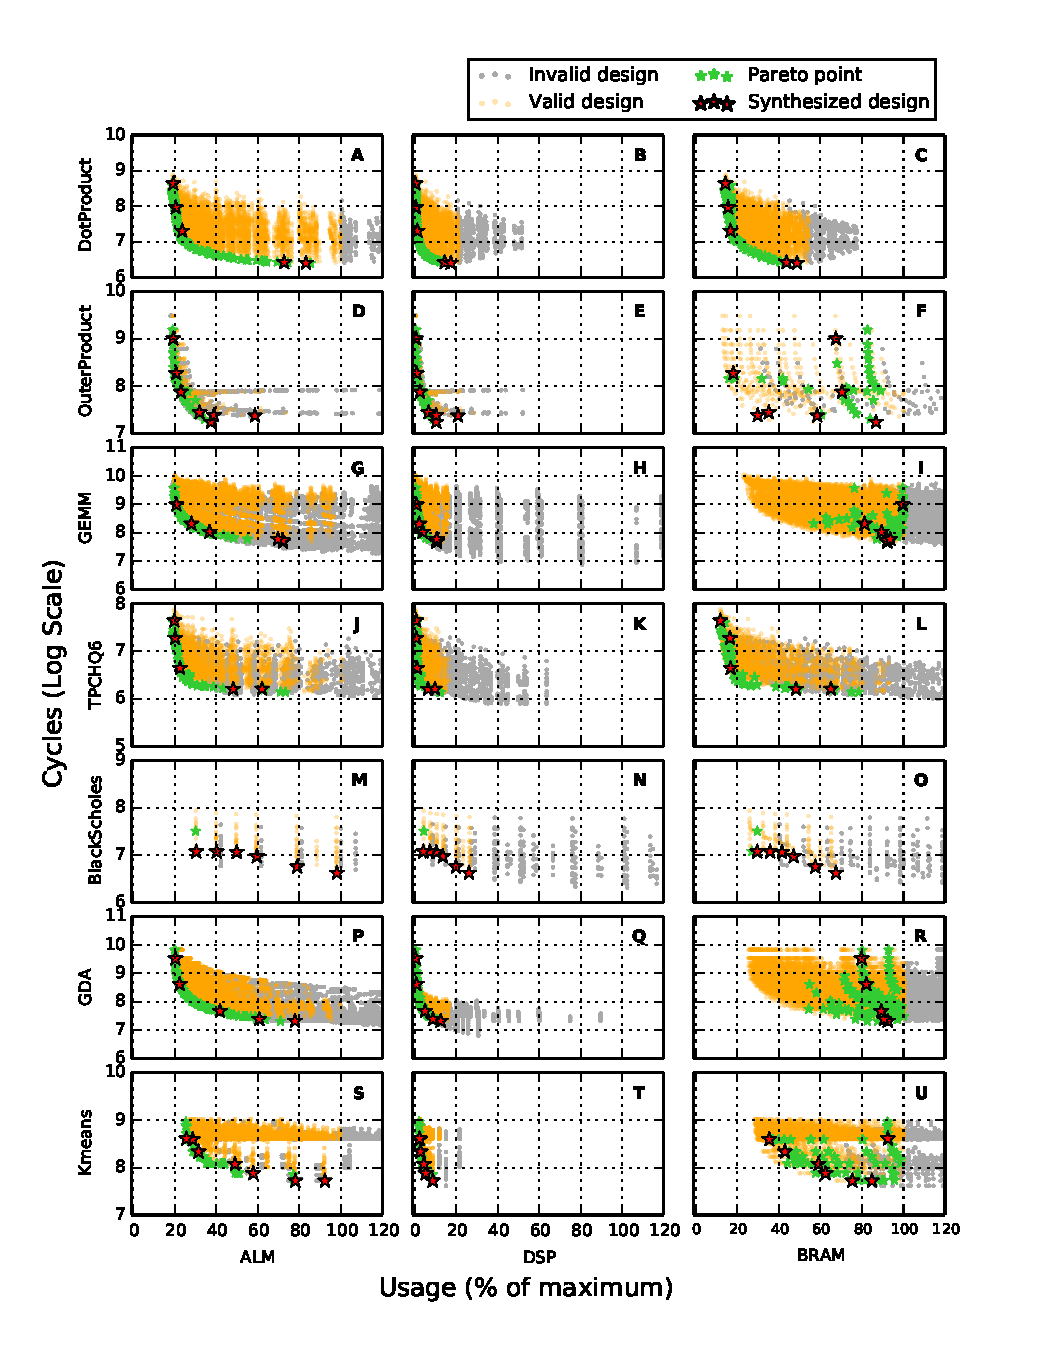
\includegraphics[width=0.95\textwidth]{figs/tradeoff.pdf}
\caption{Results of design space exploration. Horizontal axis shows estimated ALM, DSP, and BRAM usages. Vertical axis shows runtime in cycles, given in log scale (base 10).}
\label{fig:dse}
\end{figure*}

%\begin{figure*}[ht]
\subsection{Design space exploration}
\subsubsection{Pareto-optimality analysis}
In this section we show the Pareto-optimal curves of each benchmark derived from estimators.
%
Figure~\ref{fig:dse} shows the design space scatter plots for all benchmarks in
Table~\ref{t:benchmarks}. A design point is considered
invalid if its resource requirement for at least one type of resource exceeds the maximum
available amount on the target device. Pareto-optimal designs along the dimensions of execution time
and ALM utilization are highlighted for each benchmark through all three resource plots.
We now analyze each benchmark in detail.

\textbf{Dot product} (Figure~\ref{fig:dse} A,B,C) is a memory-bound benchmark. Peak execution
time is reached by balancing tile loads and computation. Inner and outer loop parallelization allows us to
quickly reach close to the input bandwidth. Runtimes of designs with \emph{MetaPipe}s then slowly decrease as parallelization
increases once the dominant stage becomes the dot product reduction tree. In \emph{dotproduct}, designs with \emph{MetaPipe} consume less resources than those with \emph{Sequential} for the same performance. \emph{Sequential}s require larger tile sizes and more parallelism to match \emph{MetaPipe} performance.

\textbf{Outer product} (Figure~\ref{fig:dse} D,E,F) represents both a BRAM and memory bound benchmark. For $2N$ inputs,
the total BRAM requirement is $2N + N^2$ to store the input and output tiles, meaning the BRAM requirement
increases quadratically with increases in input tile size. The highest performing designs for outer product do not use
\emph{MetaPipes} to overlap loading and storing of tiles. This is because the overhead due to main memory contention from overlapping
tile loads and stores turns out to be higher than the cost of executing each stage sequentially.

\textbf{GEMM} (Figure~\ref{fig:dse} G,H,I) contains a lot of temporal and spatial locality. From Figure~\ref{fig:dse}(I), Pareto-optimal designs for \emph{gemm}
occupy almost all BRAM resources on the board. Intuitively, this is  because good designs for \emph{gemm}
maximize locality by retaining large, two dimensional chunks of data in on-chip memory.
%However, as seen in Figure~\ref{fig:dse}(G), \emph{gemm} is also limited by the
%number of ALMs due to the large number of floating point operations being done in parallel.

\textbf{TPC-H Q6} (Figure~\ref{fig:dse} J,K,L) exhibits behavior typical of memory intensive applications. Performance reaches a maximum threshold
with increased tile size because of overlapping memory access and compute.

\textbf{BlackScholes} (Figure~\ref{fig:dse} M,N,O) streams through multiple large arrays and performs complex floating point computations
on the input data. Points along the same vertical bar in Figure~\ref{fig:dse}(M) share the same inner loop parallelization
factor. Increasing parallelization improves performance by increasing utilization of the available off-chip memory bandwidth.
Our model suggests that increasing the inner loop parallelization would continue to scale
performance until a parallelization of 16, around which point \emph{blackscholes} would be memory bound. Because there are not enough compute resources are available to implement a parallelization factor of 16, \emph{blackscholes} is ALM bound.

\textbf{GDA} (Figure~\ref{fig:dse} P,Q,R) possesses higher degrees of spatial locality. Because of this, \emph{gda} exhibits compute-bound behavior, where execution time
decreases steadily with increased resource utilization, as seen in Figure~\ref{fig:dse}(P). The critical resource is again BRAM. This is because BRAM usage increases with parallelization due to the creation of
more banks with fewer words per bank, which can cause under-utilization of the capacity of individual BRAMs.

\textbf{K-Means} (Figure~\ref{fig:dse} S,T,U) is bound by the number of ALMs. The critical path in this application is the distance computation done comparing an input point to each centroid.
The number of floating point operations to be done to keep up with main memory bandwidth is therefore proportional to $K \times D$, where $D$ is the number of dimensions in one point.
The performance of \emph{kmeans} is therefore limited by the number of ALMs on the FPGA, as not enough are available to perform all $K \times D$ operations in parallel.
Like GDA, \emph{kmeans} is also limited by BRAMs due to under-utilization of BRAM capacity with increased banking factors.




From our experiments, we observe that capturing parallelism at multiple levels using \emph{MetaPipe}s enables us to generate
efficient designs. In addition, effective management of on-chip BRAM resources is critical to good designs
as BRAM resources are the limiting factor for performance scaling in most of our benchmarks.
%\begin{figure*}[ht]



\subsubsection{Speed of exploration}
We compare the speed of our estimation and design space exploration with
Vivado HLS~\cite{vivadohls}, a commercial high-level synthesis tool from Xilinx.
Our evaluation uses the GDA example in Figure~\ref{fig:gda-hls} as input to the high-level synthesis tool, and the GDA
design in Figure~\ref{fig:gda-graph} as input to our design space exploration tool. Design parameters
for the high-level synthesis tool are the unrolling factors. We also include a pipeline directive
toggle for each loop in the design. For DHDL, we vary all design parameters
specified in Figure~\ref{fig:gda-code}. Speed
is measured by comparing the average estimation speed per point for 250 design points for each tool.
In our experiments, our analysis takes 5 to 29 milliseconds per design depending on the size of the application's intermediate representation.Analysis of GDA also takes 17 milliseconds per design.

\begin{table}
\centering\footnotesize
\begin{tabular}{lcc}
\toprule
{\bf Our approach}  & {\bf Vivado HLS restricted\textsuperscript{$\dagger$}} & {\bf Vivado HLS full} \\ \midrule
0.017s / design     & 4.75s / design               & 111.06s / design      \\ \midrule
\end{tabular}
\textsuperscript{$\dagger$}Vivado HLS restricted design space ignores outer loop pipelining
\caption{Average estimation time per design point.}
%The Vivado HLS design space does not include outer loop pipelining.
\label{t:speeds}
\end{table}

Table~\ref{t:speeds} shows a comparison between estimation speeds from our toolchain and Vivado HLS.
The ``restricted'' column refers to the average time spent per design over points whose outer loop ($L1$, in Figure~\ref{fig:gda-hls})
is not pipelined with a pipeline directive. The ``full'' version refers to all design points where 30 of the 250 points
have a pipeline directive to enable outer loop pipelining. We observe the following:
\begin{itemize}
  \item Our estimation tool is 279$\times$ faster than the ``restricted'' space exploration, and 6533$\times$ faster than the ``full'' space exploration.
  \item Compared to Vivado HLS, our estimation time is not sensitive to design parameter inputs. Estimation time for Vivado HLS increases
    dramatically when the outer loop is pipelined in GDA because the tool completely unrolls all inner loops
    before pipelining the outer loop. This creates a large graph that complicates scheduling. Our approach does not
    suffer from this limitation because we explicitly capture pipelines in parameterized templates such as \emph{Pipe} and
    \emph{MetaPipe}, thereby capturing outer loop pipelining more naturally.
\end{itemize}

% \begin{figure}
% \centering
% %%% trim = left, bottom, right, top
% \begin{subfigure}[t]{0.45\linewidth}
% 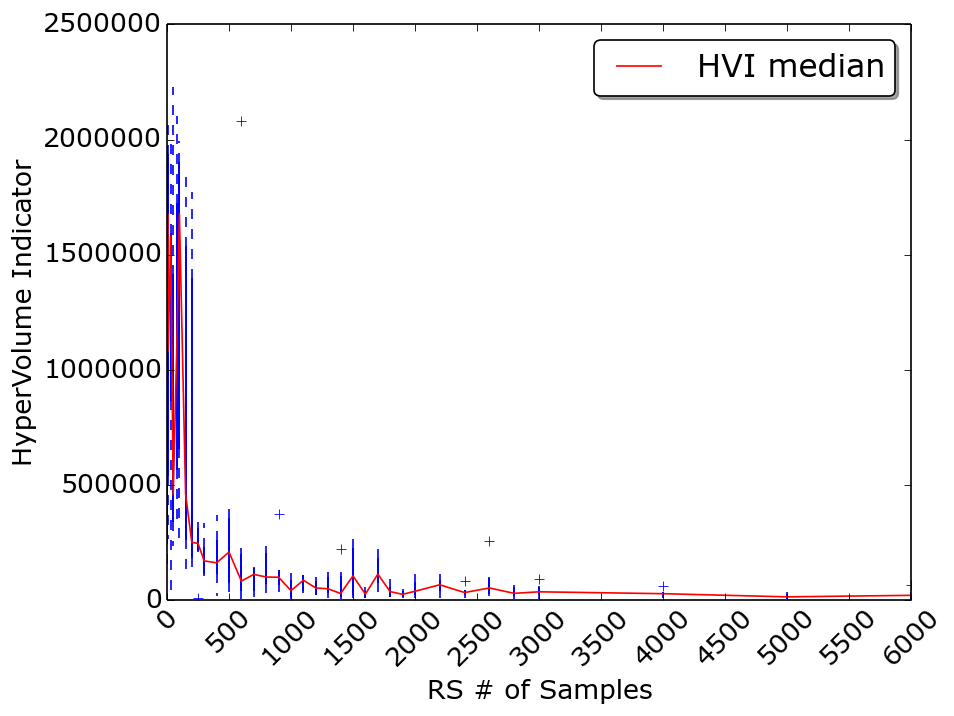
\includegraphics[width=\linewidth]{images/DSE/hvi_5NumberSummary_median.png}
% \subcaption{HyperMapper HVI versus initial random samples ($R$) five number summary.}
% \label{hvi_samples}
% \end{subfigure}\hspace{15pt}
% ~
% \begin{subfigure}[t]{0.45\linewidth}
% 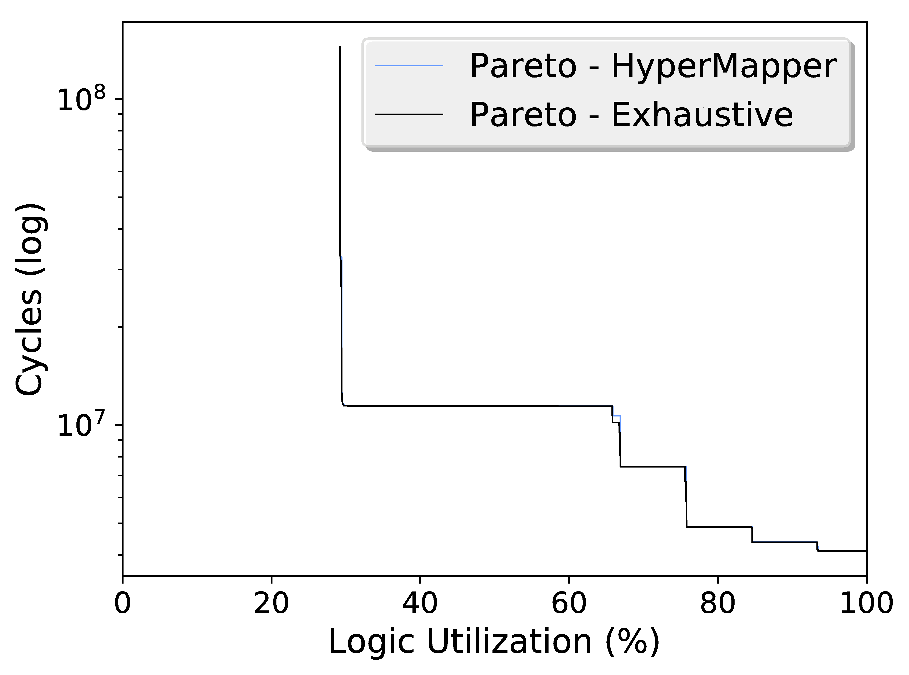
\includegraphics[clip, trim=0.0cm 0.0cm 0.0cm 0.0cm, width=\linewidth]{figs/output_pareto_blackscholes.pdf}
% \subcaption{Exhaustive and HyperMapper ($R$=1000) generated Pareto curves. }
% \label{paretos}
% \end{subfigure}

% \vspace{-10pt}
% \caption{Design space tuning on \emph{BlackScholes}.}
% \label{figHVI}
% \end{figure}

% \begin{table}[ht]
% \centering
% \caption{Runtime to reach accuracy of TODO\% and corresponding variance for design tuning with heuristic search and HyperMapper.\vspace{-10pt}}
% \label{tableDSE}

% \fontsize{7}{9}\selectfont
% \begin{tabular}{llrrrrr}
%                       & \multicolumn{2}{c}{\textbf{Space Size}} & \multicolumn{2}{c}{\textbf{Heuristic}} & \multicolumn{2}{c}{\textbf{HyperMapper}} \\
%                       & \mc{Total} & \mc{Pruned}    & \mc{Time} & \mc{Var}  &   \mc{Time} & \mc{Var} \\ \midrule
%   %\bf{Dot Product}   & 117,964,800      & 1,085,952            &              &                &                &               \\ \midrule  
%   %\bf{Outer Product} & 16,588,800       & 31,068               &              &                &                &               \\ \midrule
%   \bf{BS}             & 7.7$\times 10^4$  & 6.7$\times 10^2$    &              &                &                &               \\ \midrule
%   \bf{GDA}            & 3.0$\times 10^{10}$ & 4.6$\times 10^6$  &              &                &                &               \\ \midrule
%   \bf{GEMM}           & 2.6$\times 10^8$  & 1.4$\times 10^5$   &              &                &                &               \\ \midrule
%   \bf{KMeans}         & 2.1$\times 10^6$  & 1.9$\times 10^4$   &              &                &                &               \\ \midrule
%   \bf{SW}             & 2.1$\times 10^6$  & 3.3$\times 10^4$   &              &                &                &               \\ \midrule
%   \bf{TQ6}            & 3.5$\times 10^9$  & 2.3$\times 10^6$   &              &                &                &               \\ \bottomrule
% \end{tabular}
% \end{table}


\subsection{Spatial Portability}

\begin{table}
\centering
\caption{Runtimes (ms) of tuned designs on ZC706, followed by runtimes and speedup~($\times$) of directly porting these designs to the VU9P, then runtimes and successive speedup over ported designs when tuned for the VU9P. The \emph{Total} column shows the cumulative speedup. \vspace{-5pt} }
\label{fig:zynq_comp}

\centering
\fontsize{7}{9}\selectfont
\begin{tabular}{l d{2.1} d{2.1} d{2.1} d{2.1} d{2.1} d{2.1}}
   \bf{FPGA}      & \mc{ZC706}  & \multicolumn{4}{c}{\bf VU9P}                                       & \mc{Total}     \\ 
   \bf{Design}    & \mc{Tuned}  & \multicolumn{2}{c}{\bf Ported}   & \multicolumn{2}{c}{\bf Tuned}    &               \\ \toprule

                  & \mc{Time}   & \mc{Time}  & \mc{$\times$}       & \mc{Time}  & \mc{$\times$}       & \mc{$\times$} \\ \midrule
   \ml{BS}        & 89.0        & 35.6       & 2.5                 & 3.8        & 9.4                 & 23.4          \\ \midrule
   \ml{GDA}       &  8.4        & 3.4        & 2.5                 & 1.3        & 2.6                 & 6.5           \\ \midrule
   \ml{GEMM}      & 2226.5      & 1832.6     & 1.2                 & 878.5      & 2.1                 & 2.5           \\ \midrule
   \ml{KMeans}    & 358.4       & 143.4      & 2.5                 & 53.3       & 2.7                 & 6.7           \\ \midrule
   \ml{PageRank}  & 1299.5      & 1003.3     & 1.3                 & 587.4      & 1.7                 & 2.2           \\ \midrule
   \ml{SW$^\dag$} & 1.3         &  0.5       & 2.5                 & 0.5        & 1.0                 & 2.5           \\ \midrule
   \ml{TQ6}       & 69.4        & 15.0       & 4.6                 & 14.0       & 1.1                 & 5.0           \\ \bottomrule
   
   \multicolumn{7}{l}{\vspace{10pt}\footnotesize{ $^\dag$SW with 160 base pairs, the largest to fit on the ZC706.}}
\end{tabular}
\vspace{-10pt}
\end{table}

We next demonstrate the portability of Spatial code by targeting two different FPGA architectures; (1) the Zynq ZC706 SoC board, and (2) The Virtex Ultrascale+ VU9P on the Amazon EC2 F1.
Designs on the VU9P use a single DRAM channel with a peak bandwidth of 19.2 GB/s. The ZC706 is much smaller than the VU9P in terms of FPGA resource and has a smaller DRAM bandwidth of 4.26 GB/s.
We target both the ZC706 and VU9P from the same Spatial code for all benchmarks listed in Table~\ref{t:hls_comp}. Benchmarks are tuned for each target using
target-specific models with automated DSE. Clock frequency is fixed at 125 MHz for both FPGAs. 

Table~\ref{fig:zynq_comp} shows the speedups achieved on the VU9P over the ZC706. The results show that not only can the same Spatial source code be ported
to architectures with different capabilities, the application can also be automatically tuned to better take advantage of resources in each target.
Compute-bound benchmarks \emph{BlackScholes}, \emph{GDA}, \emph{GEMM}, \emph{K-Means} achieve speedups of up to $23\times$ on the VU9P over the ZC706. Porting these designs to the VU9P alone has a $1.2\times$ to $2.5\times$ due to increased main memory bandwidth, but a majority of the benefit of the larger FPGA comes from tuning the parallelization factors to use more resources. 
While \emph{SW} is also compute bound, the size of the dataset was limited by the smaller FPGA. In this case, the larger capacity of the VU9P does not improve runtime, but instead allows handling of larger datasets. 

Memory-bound benchmark \emph{TPC-H Q6} benefits from the higher DRAM bandwidth available on the VU9P. Porting this benchmark immediately gives a $4.6\times$ runtime improvement from the larger main memory bandwidth, while further parallelizing controllers to create more parallel address streams to DRAM helps the application make better use of this bandwidth. \emph{PageRank} is also bandwidth-bound, but the primary benefit on the VU9P comes from specializing the memory controller to maximize utilized bandwidth for sparse accesses.


% \begin{table}
% \caption{Speedup of VU9P over ZC706. \vspace{-10pt} }
% \label{fig:zynq_comp}

% \fontsize{8}{10}\selectfont
% \begin{tabular}{cccccc} 
% \bf{GDA}     & \bf{GEMM}    & \bf{K-Means} & \bf{PageRank} & \bf{SW}      & \bf{TQ6} \\ \hline
% 2.54$\times$ & 2.53$\times$ & 1.84$\times$ & 2.21$\times$  & 1.74$\times$ & 4.97$\times$  \\ \hline
% \end{tabular}
% \end{table}




\begin{table}
\centering
\caption{Plasticine DRAM bandwidth, resource utilization, runtime, and speedup ($\times$) over VU9P FPGA. \vspace{-5pt} }
\label{table:plasticine_eval}

\centering
\fontsize{7}{7}\selectfont
\resizebox{0.99\columnwidth}{!}{
  \begin{tabular}{m{0.5cm} d{2.1} d{2.1} d{2.1} d{2.1} d{2.1} d{2.1} r }
  \toprule
                 & \multicolumn{2}{c}{\bf Avg DRAM } & \multicolumn{3}{c}{\bf Resource }        & \mc{}     & \mc{} \\
                 & \multicolumn{2}{c}{\bf BW (\%)}   & \multicolumn{3}{c}{\bf Utilization (\%)} & \mc{Time} & \mc{$\times$} \\
   \bf{App}     & \mc{Load}    & \mc{Store} & \mc{PCU}  & \mc{PMU}  & \mc{AG}   & \mc{(ms)} & \mc{} \\ \midrule
   \ml{BS}       & 77.4        & 12.9       & \mb{\hspace{1pt}73.4} & 10.9      & 20.6      & 2.33      & 1.6   \\
   \ml{GDA}      & 24.0        & 0.2        & \mb{\hspace{1pt}95.3} & 73.4      & 38.2      & 0.13      & 9.8   \\
   \ml{GEMM}     & 20.5        & 2.1        & \mb{\hspace{1pt}96.8} & 64.1      & 11.7      & 15.98     & 55.0  \\
   \ml{KMeans}   & 8.0         & 0.4        & \mb{\hspace{1pt}89.1} & 57.8      & 17.6      & 8.39      & 6.3   \\
   \ml{TQ6}      & \mb{\hspace{2pt}97.2}   & 0.0        & 29.7      & 37.5      & \mb{70.6} & 8.60      & 1.6   \\

\bottomrule
\end{tabular}}
\vspace{-10pt}
\end{table}


Finally, we demonstrate the portability of Spatial beyond
FPGA architectures by extending the compiler to map
the Spatial IR to target our proposed Plasticine CGRA~\cite{plasticine}. Plasticine is a
two-dimensional array of compute (PCUs) and memory
(PMUs) tiles with a statically configurable interconnect
and address generators (AG) at the periphery to perform
DRAM accesses. The Plasticine architecture is a significant departure
from an FPGA, with more constraints on memory banking and computation, including
fixed size, pipelined SIMD lanes.

We simulate Plasticine with  a $16 \times 8$ array of 64 compute and 64 memory tiles, with a 1 GHz clock and a main memory with a DDR3-1600 channel with 12.8 GB/s peak bandwidth.
Table~\ref{table:plasticine_eval} shows the DRAM bandwidth, resource utilization, runtime, and speedup of the Plasticine CGRA over the VU9P for a subset of benchmarks.

Streaming, bandwidth-bound applications like \emph{TPC-H Q6} efficiently exploit about 97\% of the available DRAM bandwidth.
Compute-bound applications \emph{GDA}, \emph{GEMM}, and \emph{K-Means} use around 90\% of Plasticine's compute tiles.
Plasticine's higher on-chip bandwidth also allows these applications to better utilize the compute resources, giving these applications speedups of $9.9\times$, $55.0\times$, and $6.3\times$.
Similarly, the deep compute pipeline in \emph{BlackScholes} occupies 73.4\% of compute resources after being split across multiple tiles, 
giving a speedup of $1.6\times$. 

%We implemented comparable versions of each of our benchmarks in C++ and synthesized them
%using HLS and SDAccel tools.  There are certain constructs in Spatial that allow
%certain algorithms to be expressed more concisely and in slightly different, but intuitive, ways that
%expose the strengths of the language.  Each application exhibits certain characteristics which 
%can be exploited by certain aspects in the programming paradigms of Spatial and HLS. Specifically,
%they can be characterized as compute-bound applications and memory-bound applications, with some
%tradeoff between the two depending on design decisions.  While HLS is the industry standard for
%exposing FPGAs to domain experts, our results show that Spatial is a suitable alternative that can
%lead to better designs for certain algorithms with less overhead.

%Spatial is a suitable platform for the designer who is interested in making the most of the
%available resources, as it allows quick design tradeoffs in the app without needing to use complex pragmas throughout the app.
%In applications that are memory bound, such as AES, BlackScholes, and Sobel, we would expect that neither
%design could acheive significantly better speedup since they have access to the same DRAM interfaces.  
%For compute-bound applications, such as Kmeans, GEMM, and GDA, there is a large, interesting design space that
%Spatial can quickly expose to the user.

%\begin{figure}
%\centering
%\includegraphics[width=1\columnwidth, trim=0.5cm 0.9cm 1.0cm 0]{figs/f1_comp.png}
%\caption{Speedup and resource utilization comparisons with SDAccel on F1.}
%\label{fig:f1_comp}
%\end{figure}

% \subsection{Portability Across FPGAs and CGRAs}
% We demonstrate the applicability of Spatial to beyond FPGA architectures by extending the compiler
% to map Spatial IR to the Plasticine CGRA~\cite{plasticine}. Plasticine is a two-dimensional array of compute (PCUs) and memory (PMUs) tiles
% with a statically configurable interconnect and address generators (AG) at the periphery to perform DRAM accesses.
% Plasticine is a significant departure from FPGA with different kinds of constraints on memory banking and parallelization.

% Similar to the FPGA, we construct area and runtime models specific to Plasticine, and drive the design space exploration to tune
% benchmarks to Plasticine. Compiling to Plasticine then involves lowering the Spatial IR to a target-specific IR for the Plasticine low-level mapping compiler,
% which outputs a configuration bitstream. Resource utilization reports are obtained from the low-level compiler.
% Execution times are measured by simulating the generated bitstream in a cycle-accurate fashion at a clock frequency of 1 GHz. 



%Fortunately, due to the locality exhibited by these applications, designs with large tile sizes that do not maximize the off-chip
%bandwidth are capable of achieving comparable performance to the ones that have 100\%
%compute unit utilization. Hence, the best performing design point shown in
%Table~\ref{table:plasticine_eval} does not correspond to the design with 100\% compute utilization.

%Therefore, the given architecture cannot fit unrolling the outer loop by more than 1 without 
%exceeding 100\% PCU utilization. 
%\todo{K-Means is a sequential iterative convergence algorithm that neither outer loop nor
%inner loop that computes the new centroids can be parallelized.} As a result, we could not maximize
%either bandwidth or resource.}

%For application that are not memory-bound, yet Plasticine is not able to take larger
%unrolling factors, such as BlackScholes and K-Means, Plasticine still achieves roughly $4-7\times$
%speedup compared to F1 due to its higher clock frequency.

%Figure~\ref{fig:gemm_dse} shows the design space of GEMM on Plasticine. The bottom edged circles are
%designs with large tile size that better capture locality. The dark large circles on the right are 
%designs with good PCU and PMU utilization, and high DRAM load bandwidth as result of outer loop
%unrolling. 



%\begin{figure}
%\centering
%\includegraphics[width=1\columnwidth]{figs/GEMM_Blocked.png}
%\caption{Design space for GEMM on Plasticine}
%\label{fig:gemm_dse}
%\end{figure}

%\begin{figure}
%\centering
%\begin{minipage}{.5\linewidth}
  %\centering
  %\includegraphics[width=1\linewidth]{reg_K-FOLD}
  %\caption{Regularization}
  %\label{fig:reg}
%\end{minipage}%
%\end{figure}
%\subsection{GEMM Case Study}
%\gist{gemm}

\chapter{Argon}
\label{argon}
\chapter{Conclusions}
\label{conclusion}
With the end of Dennard scaling and the slow death of Moore's Law, the period
of ``free'' performance improvements on conventional CPU architectures is coming
to a close. As it does, computer architects and computer scientists alike are
looking to more specialized hardware architectures to continue improving
runtimes, throughput, and energy efficiency for performance critical applications.

While reconfigurable architectures like FPGAs are a natural fit for these
specialized hardware designs, their adoption has been historically limited by
their low level programming models. While ``C-to-gates'' style
high level synthesis tools have sought to fill this gap,
their ad-hoc mixture between hardware and software have made them
difficult to adopt when implementing optimized hardware designs.

Meanwhile, as performance requirements have been increasing, the demands for
improvements in abstractions in programming languages have also been increasing.
This is most clear in data analytics, and particularly in machine learning, where
new domain-specific languages are consistently being developed and improved.

If both of these trends continue, it is likely that this will result in a situation
where huge amounts of performance-critical code is being initially written and
tested in high level, hardware target agnostic domain specific languages.
This provides a perfect opportunity for compiler development.

In this dissertation, we describe a system which compiles high level domain
specific languages to reconfigurable architectures, with a particular focus on FPGAs.
We described several high level transformations required on a parallel pattern IR
in order to prepare the representation for hardware-specific lowering.
We then discussed the limitations with lowering to existing high level synthesis abstractions,
both in terms of their slow compile times - limiting design tuning opportunities - and their
inability to exploit arbitrary levels of nested parallelism to achieve better performance.
We instead proposed a new hardware abstraction for our system called Spatial,
which is designed from the ground up to serve as an intermediary between
high level languages and low level hardware designs.
We showed that, using this new abstraction, our system can
tune explore design parameter spaces 279 to 6533 times
faster than a commercial high-level synthesis tool, and produce designs with average speedups
of $2.9\times$ over SDAccel.
The Spatial abstraction is also coupled with a frontend language which is more productive for power users,
which we showed to have an average of 42\% fewer lines of code when defining the same applications.

Going forward, there are still a number of open research directions for this system.
While we evaluated applications directly written in Spatial to provide a fair
comparison to HLS tools at roughly the same level of abstraction, no study has yet
been done on the source or degree of overheads of automatically produced designs
from high level DSLs. Further investigation here would ultimately yield a more robust
and tuned lowering process from higher level languages.

The current Spatial compiler has a number of areas where it can be further expanded and
improved. The memory banking analysis pass, for example, is generally fast, but has
an extremely long worst case running time. This comes down to its reliance on
iterative conflict polytope emptiness testing~\cite{Wang_banking}. Current work
at Stanford is looking at how to use heuristics to speed this up, but more theoretical
work on a faster solver for the conflict polytope could improve the worst case running time.

The design tuning strategies discussed in Section~\ref{dse} show the potential for
practical application of other design space exploration or hyper-parameter tuning
strategies. While the integration with HyperMapper presented here was a preliminary
evaluation, further work evaluating HyperMapper more in depth against random search
with heuristic pruning is ongoing.

The growing adoption of domain specific languages and the growing need for hardware
acclerators presents a huge opportunity for compiler development. The target-agnostic
nature of DSLs, combined with the huge design spaces of hardware accelerator designs,
presents a great degree of freedom for optimizations and program transformations
for compilers. Our system shows how these opportunities can be taken advantage of
in order to both present users with an extremely high level programming model while
also producing performant hardware accelerator designs.

The Spatial language and compiler is an ongoing, open source project at Stanford.
Other related documentation, publications, and code releases can be found
at \url{https://spatial.stanford.edu}.


\appendix
\bibliographystyle{plain}
\bibliography{references}
\end{document}
